% MAIN PREAMBLE 
\documentclass[12pt,letterpaper]{report}          % Single-sided printing for the library
%\documentclass[12pt,twoside]{report} % Double-sided printing

\usepackage[intlimits]{amsmath}
\usepackage{amsfonts,amssymb}
\DeclareSymbolFontAlphabet{\mathbb}{AMSb}
%\usepackage{natbib}
\usepackage{apalike}
\usepackage{float}
\usepackage[bf]{caption}       
\setcaptionmargin{0.5in}
\usepackage{fancyhdr}
%\usepackage{fancyheadings}
\usepackage{fancybox}
\usepackage{ifthen}
\usepackage{bu_ece_thesis}
\usepackage{url}
\usepackage{lscape,afterpage}
\usepackage{xspace}
\usepackage{epstopdf} 
\usepackage{subfig}
% from lyx.
\usepackage{xcolor}
\usepackage{array}
\usepackage{mathtools}
\usepackage{enumitem}
\usepackage{multirow}
\usepackage[disable]{todonotes}
% \usepackage[textsize=tiny]{todonotes}
\usepackage{cancel} % why?
\usepackage{listings} % why?
\renewcommand{\lstlistingname}{Listing}
\usepackage{amsthm}
\usepackage{wasysym}

\PassOptionsToPackage{normalem}{ulem}
\usepackage{ulem}



%%% graphicx and pdf creation
\usepackage{graphicx}
\usepackage{appendix}


\theoremstyle{plain}
\newtheorem{thm}{\protect\theoremname}
\theoremstyle{plain}
\newtheorem{lem}[thm]{\protect\lemmaname}
\theoremstyle{plain}
\newtheorem{fact}[thm]{\protect\factname}
\theoremstyle{plain}
\newtheorem{cor}[thm]{\protect\corollaryname}
\newlist{casenv}{enumerate}{4}
\setlist[casenv]{leftmargin=*,align=left,widest={iiii}}
\setlist[casenv,1]{label={{\itshape\ \casename} \arabic*.},ref=\arabic*}
\setlist[casenv,2]{label={{\itshape\ \casename} \roman*.},ref=\roman*}
\setlist[casenv,3]{label={{\itshape\ \casename\ \alph*.}},ref=\alph*}
\setlist[casenv,4]{label={{\itshape\ \casename} \arabic*.},ref=\arabic*}
\theoremstyle{definition}
\newtheorem{example}[thm]{\protect\examplename}
\theoremstyle{plain}
\newtheorem{conjecture}[thm]{\protect\conjecturename}

\usepackage{xcolor}
\usepackage{tikz-cd}
\tikzcdset{%
    triple line/.code={\tikzset{%
        double equal sign distance, % replace by double distance = 'measure' 
        double=\pgfkeysvalueof{/tikz/commutative diagrams/background color}}},
    quadruple line/.code={\tikzset{%
        double equal sign distance, % replace by double distance = 'measure'
        double=\pgfkeysvalueof{/tikz/commutative diagrams/background color}}},
    Rrightarrow/.code={\tikzcdset{triple line}\pgfsetarrows{tikzcd implies cap-tikzcd implies}},
    RRightarrow/.code={\tikzcdset{quadruple line}\pgfsetarrows{tikzcd implies cap-tikzcd implies}}
}    
\newcommand*{\tarrow}[2][]{\arrow[Rrightarrow, #1]{#2}\arrow[dash, shorten >= 0.5pt, #1]{#2}}
\newcommand*{\qarrow}[2][]{\arrow[RRightarrow, #1]{#2}\arrow[equal, double distance = 0.25pt, shorten >= 1.28pt, #1]{#2}}

\makeatother

\usepackage{babel}

\providecommand{\conjecturename}{Conjecture}
\providecommand{\casename}{Case}
\providecommand{\corollaryname}{Corollary}
\providecommand{\examplename}{Example}
\providecommand{\factname}{Fact}
\providecommand{\lemmaname}{Lemma}
\providecommand{\theoremname}{Theorem}


%\usepackage{psfrag}
%\DeclareGraphicsExtensions{.eps}   % extension for included graphics
%\usepackage{thumbpdf}              % thumbnails for ps2pdf
%\usepackage[ps2pdf,                % hyper-references for ps2pdf
%bookmarks=true,%                   % generate bookmarks ...
%bookmarksnumbered=true,%           % ... with numbers
%hypertexnames=false,%              % needed for correct links to figures !!!
%breaklinks=true,%                  % breaks lines, but links are very small
%linkbordercolor={0 0 1},%          % blue frames around links
%pdfborder={0 0 112.0}]{hyperref}%  % border-width of frames 
%                                   % will be multiplied with 0.009 by ps2pdf
%\hypersetup{
%  pdfauthor   = {Joe Graduate <joe.graduate@bu.edu>},
%  pdftitle    = {dissertation.pdf},
%  pdfsubject  = {doctoral dissertations},
%  pdfkeywords = {mathematics, science, technology},
%  pdfcreator  = {LaTeX with hyperref package},
%  pdfproducer = {dvips + ps2pdf}
%}

% customized commands can be placed here
%\newcommand{\figref}[1]{Figure~\ref{#1}}
%\newcommand{\chapref}[1]{Chapter~\ref{#1}}
%\newcommand{\latex}{\LaTeX\xspace}

\begin{document}

% front matter
% This file contains all the necessary setup and commands to create
% the preliminary pages according to the buthesis.sty option.

\title{A Dependently Typed Programming Language with Dynamic Equality}

\author{Mark Lemay}

% Phd = 2
\degree=2

\prevdegrees{B.S., Rochester Institute of technology, 2010}

\department{Department of Computer Science}

\defenseyear{2022}
\degreeyear{2022}

% For each reader, specify appropriate label {First, Second, Third},
% then name, and title. IMPORTANT: The title should be:
%   "Professor of Electrical and Computer Engineering", or similar, but it MUST NOT be:
%   Professor, Department of Electrical and Computer Engineering"  or you will be asked to reprint and get new signatures.


\reader{First}{Hongwei Xi}{Associate Professor of Computer Science}
\reader{Second}{Professor Kfoury}{Professor of Computer Science}
\reader{Third}{Marco Gaboardi}{Associate Professor of Computer Science}
\reader{Fourth}{Chris Casinghino}{Research Scientist}
% \ldots}
\todo[inline]{double check honerifics "Associate Professor" v "Professor", middle initial?}

% The Major Professor is the same as the first reader, but must be specified again for the abstract page.
\numadvisors=1
\majorprof{Hongwei Xi, PhD}{{Associate Professor of Computer Science}}

%%%%%%%%%%%%%%%%%%%%%%%%%%%%%%%%%%%%%%%%%%%%%%%%%%%%%%%%%%%%%%%%  

%                       PRELIMINARY PAGES
% According to the BU guide the preliminary pages consist of:
% title, copyright (optional), approval,  acknowledgments (opt.),
% abstract, preface (opt.), Table of contents, List of tables (if
% any), List of illustrations (if any). The \tableofcontents,
% \listoffigures, and \listoftables commands can be used in the
% appropriate places. For other things like preface, do it manually
% with something like \newpage\section*{Preface}.

% This is an additional page to print a boxed-in title, author name and
% degree statement so that they are visible through the opening in BU
% covers used for reports. This makes a nicely bound copy. Uncomment only
% if you are printing a hardcopy for such covers. Leave commented out
% when producing PDF for library submission.
%\buecethesistitleboxpage

% Make the titlepage based on the above information.  If you need
% something special and can't use the standard form, you can specify
% the exact text of the titlepage yourself.  Put it in a titlepage
% environment and leave blank lines where you want vertical space.
% The spaces will be adjusted to fill the entire page.
\maketitle
\cleardoublepage

% The copyright page is blank except for the notice at the bottom. You
% must provide your name in capitals.
\copyrightpage
\cleardoublepage

% Now include the approval page based on the readers information
% Once the approval page is approved by the Mugar Library staff, please
% comment out the "\approvalpagewithcomment" line and uncomment "\approvalpage"
\approvalpagewithcomment
%\approvalpage
\cleardoublepage

% Here goes your favorite quote. This page is optional.
\newpage
%\thispagestyle{empty}
\phantom{.}
\vspace{4in}

\begin{singlespace}
\begin{quote}
  What I mean is that if you really want to understand something, the best way is to try and explain it to someone else. That forces you to sort it out in your own mind. And the more slow and dim-witted your pupil, the more you have to break things down into more and more simple ideas. And that’s really the essence of programming. By the time you’ve sorted out a complicated idea into little steps that even a stupid machine can deal with, you’ve certainly learned something about it yourself. The teacher usually learns more than the pupil. Isn’t that true?

  \hfill{Douglas Adams, Dirk Gently's Holistic Detective Agency}
\end{quote}
\end{singlespace}

% \vspace{0.7in}
%
% \noindent
% [The descent to Avernus is easy; the gate of Pluto stands open night
% and day; but to retrace one's steps and return to the upper air, that
% is the toil, that the difficulty.]

\cleardoublepage

% The acknowledgment page should go here. Use something like
% \newpage\section*{Acknowledgments} followed by your text.
\newpage
\section*{\centerline{Acknowledgments}}
First and foremost my fiancé Stephanie Savir, I could not have finished this without her support. %% And she fixed some typeos
% 2021 was a rough year, and her positivity
 
Boston University is an excellent school to learn Computer Science.
It is so full of intelligent, passionate, and kind people that any list of people will feel incomplete.
Given that I especially want to thank Dr.(!) Tomislav Petrovic his wife Ana and their adorably strong willed children for the longest friendship at BU;
Qiancheng Fu, Cheng Zhang, and William Blair for their discussions, collaborations and friendship;
and my advisor Dr. Hongwei Xi who has been more supportive than I would have thought possible.
Also he is a genius.
Thanks to Malavika Vishwanath of the Writing Assistance center for reviewing drafts of this thesis.
Finally to the administrators (especially Kori MacDonald) who have always managed to get paperwork where it is needed to go in spite of me.

My family has also supported, encouraged and tolerated this thesis process.
Matt Lemay and his wife Alex and their dog Lilly were always ready to provide a needed destraction and encouragement\footnote{``Cs get degrees bro''}.
My parents Bob and Carol Lemay also need to be thanked for their support.

Our roommates and friends Eric Gibbs and Jess Noble (and pets Padfoot, Crookshanks, Ms. Noris) for keeping us sane(?) during the pandemic lockdown.
There are too many other friends to list here, but special thanks to Ramsay Hoguet for proofreading a draft of this thesis.

\todo[inline]{Anonoumous people from discord}
\todo[inline]{Steph's Fam?}
\todo[inline]{Alley S for chairing if not recorded elsewhere}
\todo[inline]{other people?}
\todo[inline]{sign name?}
% \vskip 1in

% \noindent
% Mark Lemay\\
% % Professor\\
% % ECE Department
\cleardoublepage

% The abstractpage environment sets up everything on the page except
% the text itself.  The title and other header material are put at the
% top of the page, and the supervisors are listed at the bottom.  A
% new page is begun both before and after.  Of course, an abstract may
% be more than one page itself.  If you need more control over the
% format of the page, you can use the abstract environment, which puts
% the word "Abstract" at the beginning and single spaces its text.

\begin{abstractpage}
Dependent types offer a uniform foundation for both proof systems and programming languages.
While the proof systems built with dependent types have become relatively popular, dependently typed programming languages are far from mainstream.

One key issue with existing dependently typed languages is the overly conservative definitional equality that programmers are forced to use.
When combined with a traditional typing workflow, these systems can be quite challenging and require a large amount of expertise to master.

This thesis explores an alternative workflow and a more liberal handling of equality.
Programmers are given warnings that contain the same information as the type errors that would be given by an existing system.
Programmers can run these programs optimistically, and they will behave appropriately unless a direct contradiction confirming the warning is found.

This is achieved by localizing equality constraints using a new form of elaboration based on bidirectional type inference.
These local checks, or casts, are given a runtime behavior (similar to those of contract and monitors).
The elaborated terms have a weakened form of type soundness, they will not get stuck without an explicit counter example.

The language explored in this thesis will be a calculus of constructions like language with recursion, \tit, data types with dependent indexing and pattern matching.

Several meta-theoretic results will be presented.
The key result is that the core language, called the \textbf{cast system}, ``will not get stuck without a counter example''; a result called \textbf{cast soundness}.
A proof of cast soundness is fully worked out for the fragment of the system without user defined data, and a Coq proof is available. Several other properties based on the gradual guarantees of gradual typing are also presented.
In the presence of user defined data and pattern matching these properties are conjectured to hold.

A prototype implementation of this work is available.

\todo[inline]{review of not new stuff}
\end{abstractpage}
\cleardoublepage

% Now you can include a preface. Again, use something like
% \newpage\section*{Preface} followed by your text

% Table of contents comes after preface
\tableofcontents
\cleardoublepage

% If you do not have tables, comment out the following lines
% \newpage
% \listoftables
% \cleardoublepage

% If you have figures, uncomment the following line
\newpage
\listoffigures
\cleardoublepage

% List of Abbrevs is NOT optional (Martha Wellman likes all abbrevs listed)
\chapter*{List of Abbreviations}

% {\bf The list below must be in alphabetical order as per BU library instructions or it will be returned to you for re-ordering.}

\todo[inline]{would be nice to match the formmatting of the above, but I think this satisfies the requirements}
% https://tex.stackexchange.com/questions/492175/how-to-generate-list-of-abbreviations-in-latex
% https://tex.stackexchange.com/questions/86666/how-to-create-both-list-of-abbreviations-and-list-of-nomenclature-using-nomencl/87223

\printacronyms[name={}]
% \begin{center}
%   \begin{tabular}{lll}
%     \hspace*{2em} & \hspace*{1in} & \hspace*{4.5in} \\
%     CAD  & \dotfill & Computer-Aided Design \\
%     CO   & \dotfill & Cytochrome Oxidase \\
%     DOG  & \dotfill & Difference Of Gaussian (distributions) \\
%     FWHM & \dotfill & Full-Width at Half Maximum \\
%     LGN  & \dotfill & Lateral Geniculate Nucleus \\
%     ODC  & \dotfill & Ocular Dominance Column \\
%     PDF  & \dotfill & Probability Distribution Function \\
%     $\mathbb{R}^{2}$  & \dotfill & the Real plane \\
%   \end{tabular}
% \end{center}
\cleardoublepage

\newpage
\endofprelim
   
% % This file contains all the necessary setup and commands to create
% the preliminary pages according to the buthesis.sty option.

\title{A Dependently Typed Programming Language with Dynamic Equality}

\author{Mark Lemay}

% Phd = 2
\degree=2

\prevdegrees{B.S., Rochester Institute of technology, 2010}

\department{Department of Computer Science}

\defenseyear{2022}
\degreeyear{2022}

% For each reader, specify appropriate label {First, Second, Third},
% then name, and title. IMPORTANT: The title should be:
%   "Professor of Electrical and Computer Engineering", or similar, but it MUST NOT be:
%   Professor, Department of Electrical and Computer Engineering"  or you will be asked to reprint and get new signatures.


\reader{First}{Hongwei Xi}{Associate Professor of Computer Science}
\reader{Second}{Professor Kfoury}{Professor of Computer Science}
\reader{Third}{Marco Gaboardi}{Associate Professor of Computer Science}
\reader{Fourth}{Chris Casinghino}{Research Scientist}
% \ldots}
\todo[inline]{double check honerifics "Associate Professor" v "Professor", middle initial?}

% The Major Professor is the same as the first reader, but must be specified again for the abstract page.
\numadvisors=1
\majorprof{Hongwei Xi, PhD}{{Associate Professor of Computer Science}}

%%%%%%%%%%%%%%%%%%%%%%%%%%%%%%%%%%%%%%%%%%%%%%%%%%%%%%%%%%%%%%%%  

%                       PRELIMINARY PAGES
% According to the BU guide the preliminary pages consist of:
% title, copyright (optional), approval,  acknowledgments (opt.),
% abstract, preface (opt.), Table of contents, List of tables (if
% any), List of illustrations (if any). The \tableofcontents,
% \listoffigures, and \listoftables commands can be used in the
% appropriate places. For other things like preface, do it manually
% with something like \newpage\section*{Preface}.

% This is an additional page to print a boxed-in title, author name and
% degree statement so that they are visible through the opening in BU
% covers used for reports. This makes a nicely bound copy. Uncomment only
% if you are printing a hardcopy for such covers. Leave commented out
% when producing PDF for library submission.
%\buecethesistitleboxpage

% Make the titlepage based on the above information.  If you need
% something special and can't use the standard form, you can specify
% the exact text of the titlepage yourself.  Put it in a titlepage
% environment and leave blank lines where you want vertical space.
% The spaces will be adjusted to fill the entire page.
\maketitle
\cleardoublepage

% The copyright page is blank except for the notice at the bottom. You
% must provide your name in capitals.
\copyrightpage
\cleardoublepage

% Now include the approval page based on the readers information
% Once the approval page is approved by the Mugar Library staff, please
% comment out the "\approvalpagewithcomment" line and uncomment "\approvalpage"
\approvalpagewithcomment
%\approvalpage
\cleardoublepage

% Here goes your favorite quote. This page is optional.
\newpage
%\thispagestyle{empty}
\phantom{.}
\vspace{4in}

\begin{singlespace}
\begin{quote}
  What I mean is that if you really want to understand something, the best way is to try and explain it to someone else. That forces you to sort it out in your own mind. And the more slow and dim-witted your pupil, the more you have to break things down into more and more simple ideas. And that’s really the essence of programming. By the time you’ve sorted out a complicated idea into little steps that even a stupid machine can deal with, you’ve certainly learned something about it yourself. The teacher usually learns more than the pupil. Isn’t that true?

  \hfill{Douglas Adams, Dirk Gently's Holistic Detective Agency}
\end{quote}
\end{singlespace}

% \vspace{0.7in}
%
% \noindent
% [The descent to Avernus is easy; the gate of Pluto stands open night
% and day; but to retrace one's steps and return to the upper air, that
% is the toil, that the difficulty.]

\cleardoublepage

% The acknowledgment page should go here. Use something like
% \newpage\section*{Acknowledgments} followed by your text.
\newpage
\section*{\centerline{Acknowledgments}}
First and foremost my fiancé Stephanie Savir, I could not have finished this without her support. %% And she fixed some typeos
% 2021 was a rough year, and her positivity
 
Boston University is an excellent school to learn Computer Science.
It is so full of intelligent, passionate, and kind people that any list of people will feel incomplete.
Given that I especially want to thank Dr.(!) Tomislav Petrovic his wife Ana and their adorably strong willed children for the longest friendship at BU;
Qiancheng Fu, Cheng Zhang, and William Blair for their discussions, collaborations and friendship;
and my advisor Dr. Hongwei Xi who has been more supportive than I would have thought possible.
Also he is a genius.
Thanks to Malavika Vishwanath of the Writing Assistance center for reviewing drafts of this thesis.
Finally to the administrators (especially Kori MacDonald) who have always managed to get paperwork where it is needed to go in spite of me.

My family has also supported, encouraged and tolerated this thesis process.
Matt Lemay and his wife Alex and their dog Lilly were always ready to provide a needed destraction and encouragement\footnote{``Cs get degrees bro''}.
My parents Bob and Carol Lemay also need to be thanked for their support.

Our roommates and friends Eric Gibbs and Jess Noble (and pets Padfoot, Crookshanks, Ms. Noris) for keeping us sane(?) during the pandemic lockdown.
There are too many other friends to list here, but special thanks to Ramsay Hoguet for proofreading a draft of this thesis.

\todo[inline]{Anonoumous people from discord}
\todo[inline]{Steph's Fam?}
\todo[inline]{Alley S for chairing if not recorded elsewhere}
\todo[inline]{other people?}
\todo[inline]{sign name?}
% \vskip 1in

% \noindent
% Mark Lemay\\
% % Professor\\
% % ECE Department
\cleardoublepage

% The abstractpage environment sets up everything on the page except
% the text itself.  The title and other header material are put at the
% top of the page, and the supervisors are listed at the bottom.  A
% new page is begun both before and after.  Of course, an abstract may
% be more than one page itself.  If you need more control over the
% format of the page, you can use the abstract environment, which puts
% the word "Abstract" at the beginning and single spaces its text.

\begin{abstractpage}
Dependent types offer a uniform foundation for both proof systems and programming languages.
While the proof systems built with dependent types have become relatively popular, dependently typed programming languages are far from mainstream.

One key issue with existing dependently typed languages is the overly conservative definitional equality that programmers are forced to use.
When combined with a traditional typing workflow, these systems can be quite challenging and require a large amount of expertise to master.

This thesis explores an alternative workflow and a more liberal handling of equality.
Programmers are given warnings that contain the same information as the type errors that would be given by an existing system.
Programmers can run these programs optimistically, and they will behave appropriately unless a direct contradiction confirming the warning is found.

This is achieved by localizing equality constraints using a new form of elaboration based on bidirectional type inference.
These local checks, or casts, are given a runtime behavior (similar to those of contract and monitors).
The elaborated terms have a weakened form of type soundness, they will not get stuck without an explicit counter example.

The language explored in this thesis will be a calculus of constructions like language with recursion, \tit, data types with dependent indexing and pattern matching.

Several meta-theoretic results will be presented.
The key result is that the core language, called the \textbf{cast system}, ``will not get stuck without a counter example''; a result called \textbf{cast soundness}.
A proof of cast soundness is fully worked out for the fragment of the system without user defined data, and a Coq proof is available. Several other properties based on the gradual guarantees of gradual typing are also presented.
In the presence of user defined data and pattern matching these properties are conjectured to hold.

A prototype implementation of this work is available.

\todo[inline]{review of not new stuff}
\end{abstractpage}
\cleardoublepage

% Now you can include a preface. Again, use something like
% \newpage\section*{Preface} followed by your text

% Table of contents comes after preface
\tableofcontents
\cleardoublepage

% If you do not have tables, comment out the following lines
% \newpage
% \listoftables
% \cleardoublepage

% If you have figures, uncomment the following line
\newpage
\listoffigures
\cleardoublepage

% List of Abbrevs is NOT optional (Martha Wellman likes all abbrevs listed)
\chapter*{List of Abbreviations}

% {\bf The list below must be in alphabetical order as per BU library instructions or it will be returned to you for re-ordering.}

\todo[inline]{would be nice to match the formmatting of the above, but I think this satisfies the requirements}
% https://tex.stackexchange.com/questions/492175/how-to-generate-list-of-abbreviations-in-latex
% https://tex.stackexchange.com/questions/86666/how-to-create-both-list-of-abbreviations-and-list-of-nomenclature-using-nomencl/87223

\printacronyms[name={}]
% \begin{center}
%   \begin{tabular}{lll}
%     \hspace*{2em} & \hspace*{1in} & \hspace*{4.5in} \\
%     CAD  & \dotfill & Computer-Aided Design \\
%     CO   & \dotfill & Cytochrome Oxidase \\
%     DOG  & \dotfill & Difference Of Gaussian (distributions) \\
%     FWHM & \dotfill & Full-Width at Half Maximum \\
%     LGN  & \dotfill & Lateral Geniculate Nucleus \\
%     ODC  & \dotfill & Ocular Dominance Column \\
%     PDF  & \dotfill & Probability Distribution Function \\
%     $\mathbb{R}^{2}$  & \dotfill & the Real plane \\
%   \end{tabular}
% \end{center}
\cleardoublepage

\newpage
\endofprelim
   
\cleardoublepage

\chapter{Introduction}
\label{chapter:Introduction}
\thispagestyle{myheadings}

\section{Introduction} % needs this for some reason?

%% why dependent types?
Writing correct programs is difficult.
While many formal methods approaches make some errors rare or impossible, they often require programmers learn additional syntax and semantics.
Dependent type systems can offer a simpler approach.
In dependent type systems, proofs and properties use the same language and meaning already familiar to functional programmers.

While the type systems of mainstream programming languages allow tracking simple properties, like $\mathtt{7:int}$ or $\mathtt{not(x):bool}$.
Dependent types allow complicated properties to be assumed and verified, such as a provably correct sorting function

\[
sort\,:\,\left(input:List\,\mathbb{N}\right)\rightarrow\Sigma ls:List\,\mathbb{N}.IsSorted\,input\,ls
\]

by providing an appropriate definition of $sort$ at that type.
From the programmer's perspective, the function arrow and the implication arrow are the same.
The proof $IsSorted$ is no different than any other term of a datatype like $List$ or $\mathbb{N}$.

The power of dependent types has been recognized for decades.
Dependent types form the backbone of several poof systems, such as Coq\cite{Coq12}, Lean\cite{10.1007/978-3-030-79876-5_37}, and Agda\cite{norell2007towards}.
\todo{not clear these are the best citations, there seems to be little consensus online about how to cite software}
They have been proposed as a foundation for mathematics\cite{Martin-Lof-1972,HoTTbook}.
Dependent types are directly used in several programming languages such as ATS\cite{DependentMLAnapproachtopracticalprogrammingwithdependenttypes} and Idris\cite{brady2013idris}, while influencing many other programing languages such as Haskell and Scala.
\todo{cite the languages/ the dependent features both? neither?}

Unfortunately, dependent types have not yet become mainstream in the software industry.
Many of the usability issues with dependent types can trace their root to the conservative nature of dependently typed equality.
This thesis illustrates a new way to deal with equality constraints by delaying them until runtime.

A fragment of the system is proven correct according to a modified view of type soundness, and several of the proofs have been validated in Coq\footnote{
available at \url{https://github.com/marklemay/dtest-coq} most work is due to Qiancheng Fu}.
The system has been prototyped\footnote{available at \url{https://github.com/marklemay/dDynamic}}.

\todo[inline]{revise last paragraph? move?}

\subsection{Example}

Dependent type systems can prevent an index-out-of-bounds error when trying to read the first element of a list.
A version of the following type checks in virtually all dependent type systems:

\todo[inline]{expand this example? perhaps at the head of a constant vector first? ``and this reasoning can be abstracted under functions'' }

\begin{align*}
\mathtt{Bool} & :*,\\
\mathtt{Nat} & :*,\\
\mathtt{Vec} & :*\rightarrow\mathtt{Nat}\rightarrow*,\\
\mathtt{add} & :\mathtt{Nat}\rightarrow\mathtt{Nat}\rightarrow\mathtt{Nat},\\
\mathtt{rep} & :\left(A:*\right)\rightarrow A\rightarrow\left(x:\mathtt{Nat}\right)\rightarrow\mathtt{Vec\,}A\,x,\\
\mathtt{head} & :\left(A:*\right)\rightarrow\left(x:\mathtt{Nat}\right)\rightarrow\mathtt{Vec}\,A\,\left(\mathtt{add}\,1\,x\right)\rightarrow A
\end{align*}
\[
\vdash\lambda x.\mathtt{head}\,\mathtt{Bool}\,x\,\left(\mathtt{rep}\,\mathtt{Bool}\,\mathtt{true}\,\left(\mathtt{add}\,1\,x\right)\right)\,:\,\mathtt{Nat}\rightarrow\mathtt{Bool}
\]

\todo[inline]{make this a ``code'' example?}

Where $\rightarrow$ is a function and $*$ means that the function results in a type.
$\mathtt{Vec}$ is a list indexed by the type of element it contains and its length.
$\mathtt{Vec}$ is a type that depends on its length.
$\mathtt{rep}$ is a dependent function that produces a list containing a type with a given length by repeating its input that number of times.
$\mathtt{head}$ is a dependent function that expects a list of length $\mathtt{add}\,1\,x$, returning the first element of that non-empty list.

There is no risk that $\mathtt{head}$ inspects an empty list.
Luckily in the example the $\mathtt{\mathtt{rep}\,\mathtt{Bool}\,\mathtt{true}\,\left(\mathtt{add}\,1\,x\right)}$ function will return a list of length $\mathtt{add}\,1\,x$, exactly the type that is required.

%% This example only scratches the surface of what is possible with dependent types.

Unfortunately, programmers often find dependent type systems difficult to learn and use.
This resistance has limited the ability of dependent types to reach their full potential to help eliminate the bugs that pervade software systems.
One of the deepest underlying reasons for this frustration is the way dependent type systems handle equality.

For example, the following will not type check in any conventional dependent type system with user defined addition,

\[
\cancel{\vdash}\lambda x.\mathtt{head}\,\mathtt{Bool}\,x\,\left(\mathtt{rep}\,\mathtt{Bool}\,\mathtt{true}\,\left(\mathtt{add}\,x\,1\right)\right)\,:\,\mathtt{Nat}\rightarrow\mathtt{Bool}
\]

While ``obviously'' $1+x=x+1$, in the majority of dependently typed languages, $\mathtt{add}\,1\,x\equiv\mathtt{add}\,x\,1$ is not a ``definitional'' equality.
``Definitional equality'' is the name for the conservative approximation of equality used by dependent type systems for when two types are clearly the same.
This prevents the use of a term of type
$\mathtt{Vec}\,\mathtt{Bool}\,\left(\underline{\mathtt{add}\,1\,x}\right)$
where a term of type
$\mathtt{Vec}\,\mathtt{Bool}\,\left(\underline{\mathtt{add}\,x\,1}\right)$
is expected.
Usually when dependent type systems encounter situations like this, they will give an error message and prevent the programmer from doing more work until the ``mistake'' is resolved.

In programming, types are used to avoid bad behavior.
For instance, they are often used to avoid ``stuck'' terms.
If it is the case that $\mathtt{add}\,1\,x\,=\,\mathtt{add}\,x\,1$ the program will never get stuck.
However, if there is a mistake in the implementation of $\mathtt{add}$, then it is possible $\mathtt{add}\,1\,x\,\cancel{=}\,\mathtt{add}\,x\,1$ and the program might get stuck.
For instance, if the $\mathtt{add}$ function incorrectly computes $\mathtt{add}\,8\,1=0$ the above function will ``get stuck'' on the input $8$.

While the intent and properties of the $\mathtt{add}$ function are clear to programmers from its name and type, this information is unavailable to the type system.
If the programmer made a mistake in the definition of addition, such that for some $x$, $\mathtt{add}\,1\,x\,\cancel{=}\,\mathtt{add}\,x\,1$, the system will not provide hints on which $x$ witnesses this inequality.
Worse, the type system may even make it difficult to experiment with the $\mathtt{add}$ function, which makes repairing an actual bug difficult.

Why stop programmers when there is a definitional equality ``error''? \todo{Awk, in HM it makes sense to block}

There appears to be no reason! Alternatively, we can track unclear equalities and if the program ``gets stuck'', we are able to stop the program execution and provide a concrete witness for the inequality at runtime.
If the buggy add function above is encountered at runtime, we can give a runtime error stating $\mathtt{add}\,1\,8=9\,\neq\,0=\mathtt{add}\,8\,1$.
Which is exactly the kind of specific feedback programers want when fixing bugs.

\section{A Different Workflow}

This thesis advocates an alternative usage of types. In most types systems a programmer can't run programs until the type system is convinced of their correctness\footnote{
 often requiring a graduate degree and uncommon patience}.
Where this thesis argues ``the programmer is always right (until proven wrong)''.
This philosophy will likely go over better with programmers.

More concretely, whenever possible, static errors should be replaced with
\begin{itemize}
\item static warnings containing the same information,
\item and more concrete and clear runtime errors that correspond to one of the warnings
\end{itemize}
Figure \ref{fig:intro-standard-workflow} illustrates the standard workflow from the perspective of programmers in most typed languages.
Figure \ref{fig:intro-thesis-workflow} shows the workflow that is explored in this thesis.

\begin{figure}
% \begin{lstlisting}
% edit program
% |      ^
% |      | type errors
% v      |
% Type checks
% |
% | no type errors
% v
% run program
% \end{lstlisting}

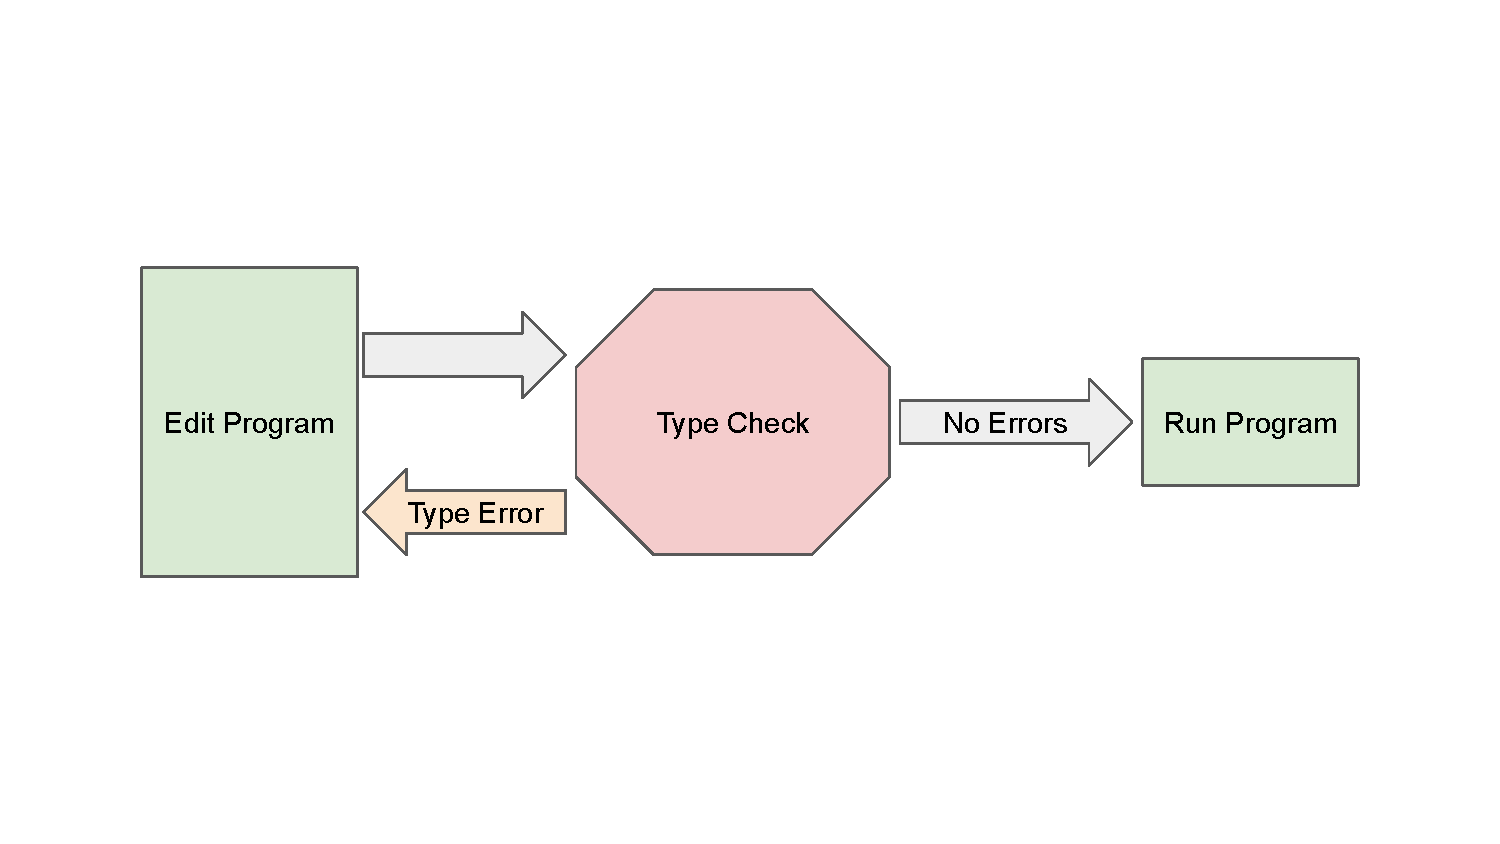
\includegraphics[width=5in]{1_intro/fig/standard-workflow.pdf}
% https://docs.google.com/presentation/d/1FSXDKsZlYFDNP8f6HprCrWV7gBRyW03PmIP0KkOprIA/edit#slide=id.g11561a4b8c2_0_0

\caption{Standard Typed Programming Workflow}
\label{fig:intro-standard-workflow}
\end{figure}

\begin{figure}
% \begin{lstlisting}
% edit program
% |     
% |     
% v
% Elaborates                     ^
% |              |               | runtime error
% | no warnings  | type warnings |
% v              v               |
%    run program   ---------------
% \end{lstlisting}
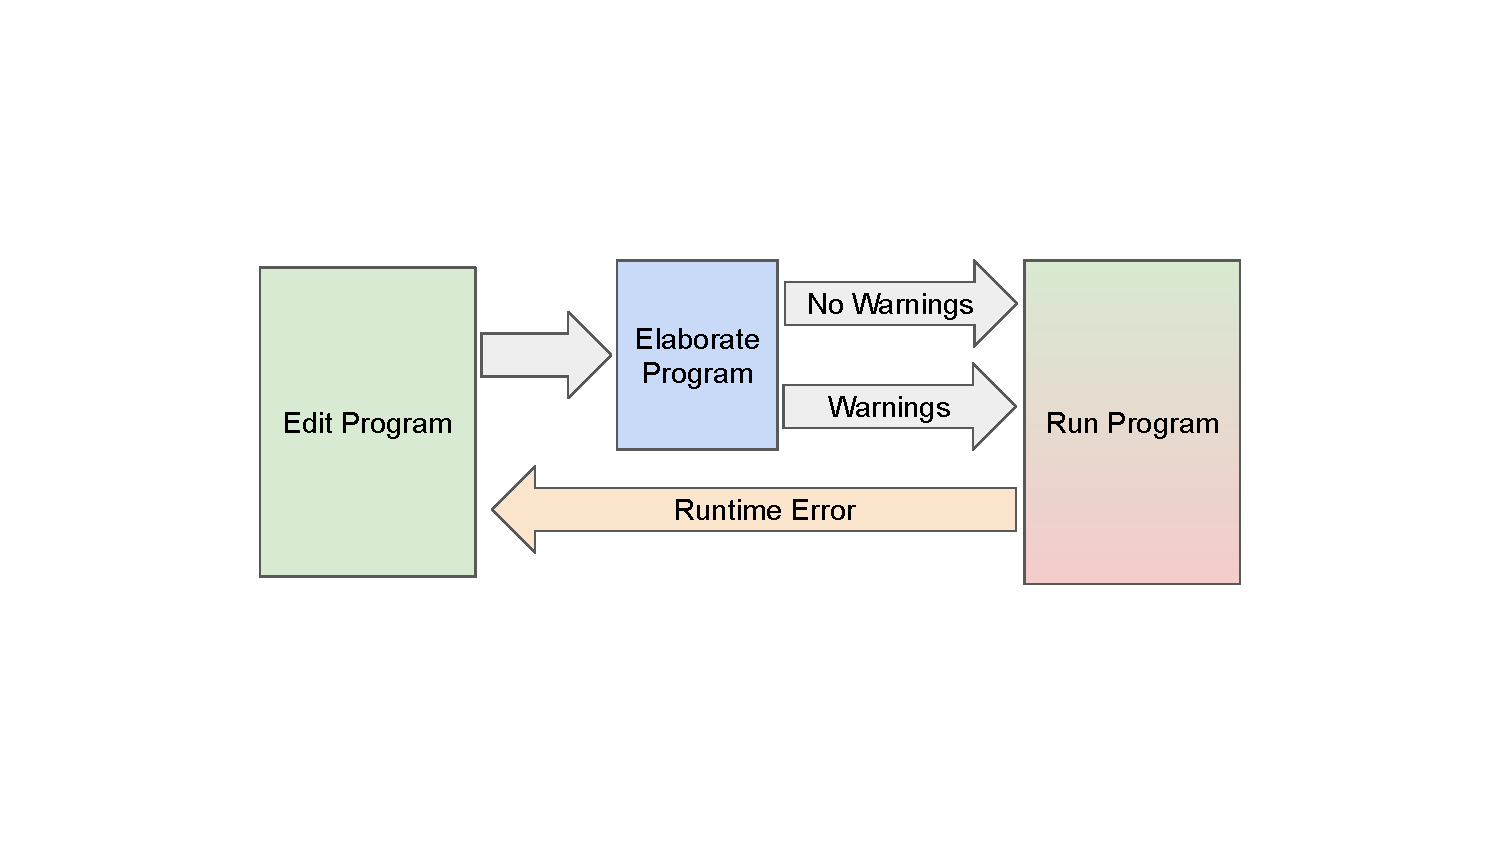
\includegraphics[width=5in]{1_intro/fig/new-workflow.pdf}
% https://docs.google.com/presentation/d/1FSXDKsZlYFDNP8f6HprCrWV7gBRyW03PmIP0KkOprIA/edit#slide=id.g11561a4b8c2_0_0

\caption{Workflow for this Thesis}
\label{fig:intro-thesis-workflow}
\end{figure}

These diagrams make it clear why there is so much pressure for type errors to be better in dependently typed programming\cite{eremondi2019framework}.
Type errors block programmers from running programs! However complaints about the type errors are probably better addressed by resolving the mismatch between the expectations of the programmer and the design of the underlying type theory.
Better worded error messages are unlikely to bridge this gap when the type system doubts $x+1=1+x$.

The standard workflow seems sufficient for type systems in many mainstream typed programming languages.
Though there is experimental evidence that even OCaml can be easier to learn and use with the proposed workflow \cite{10.1145/2951913.2951915}.
In the presence of dependent types the standard workflow is challenging for both beginners and experts, making a new approach much more critical.

\todo[inline]{
What is new here? talk about some of the prior dependent type attempts,
always a subset of syntax, or changes the syntax}

By switching to the proposed workflow, type errors become type warnings, and the programmer is free to run their program and experiment, while still presented with all the information they would have gotten from a type error (in the form of warnings).
If there are no warnings, the programmer could call their program a proof along the lines of the Curry-Howard correspondence\footnote{
  In the system presented here the programmer will need to manually verify termination
}\todo{cite?}.
If there is value in a type error it comes from the message itself and not the inconvenience it causes programmers.

The proposed workflow is necessary, since often the type system is too conservative and the programmer is correct in implicitly asserting an equality that is not provable within the system.
That the programmer may need to go outside the conservative bounds of definitional equality has been recognized since the earliest dependent type theories \cite{Martin-Lof-1972} and difficulties in dependently typed equality have motivated many research projects \cite{HoTTbook,sjoberg2015programming,cockx2021taming}.
However, these impressive efforts are still only usable by experts, since they frequently require the programmer prove their equalities explicitly\cite{HoTTbook,sjoberg2015programming}, or add custom rules into the type system \cite{cockx2021taming}.
Further, since program equivalence is undecidable in general, no system will be able to statically verify every ``obvious'' equality for arbitrary user defined data types and functions.
In practice, every dependently typed language has a way to assume equalities, even though these assumptions will result in computationally bad behavior (the program may ``get stuck'').

The proposed workflow presented in this thesis is justified by:
\begin{itemize}
\item The strict relation between warnings and runtime errors.
A runtime error will always correspond exactly to a reported warning, always validating the warning with a specific example.
\item A form of type soundness holds, programs will never ``get stuck'' unless a concrete witness of warning is found.
\item Programs that type check against a model type system will not have warnings, and therefore cannot have errors.
\item Other than warnings and errors the runtime behavior is similar to a conventional type theory.
% this is actually true, even in a normalizing theory, the runtime behavior is standard
\end{itemize}

\subsection{Example}

While the primary benefit of this system is the ability to experiment more freely with dependent types, while still getting the full feedback of a dependent type system, it is also possible to encode examples that would be unfeasible in existing systems.
This comes from accepting warnings that are justified with external mathematical or programmatic intuition, even while being theoretically thorny in dependent type theory.

For instance, here is part of an interpreter for interpreter for System F\todo{cite?}\footnote{
 System F is one of the foundational systems used to study programming languages.
 It is possible to fully encode evaluation and proofs into Agda, but it is difficult if computation, like substitution, happens in a type.
 In our system, it is possible to start with the ideal type indexed encoding and build an interpreter, without proving any properties of substitution.
} that encodes the type of the term at the type level.
The step function asserts type preservation of the interpreter in its function signature.

\begin{figure}
\begin{lstlisting}[basicstyle={\ttfamily\small}]
Ctx : * ;
Ctx = Var -> Ty;

data Ty : * {
| tv : tVar -> Ty
| arr : Ty -> Ty -> Ty
| forall : Ty -> Ty
};

data Term : Ctx -> Ty -> * {
| V : (ctx : (Var -> Ty)) -> (x : Var) ->
Term ctx (ctx x)
| lam : (ctx : Ctx) ->
(targ : Ty) -> (tbod : Ty) ->
Term (ext ctx targ) tbod ->
Term ctx (arr targ tbod)
| app : (ctx : Ctx) ->
(arg : Ty) -> (bod : Ty) ->
Term ctx (arr arg bod) ->
Term ctx arg ->
Term ctx bod
| tlam : (ctx : Ctx) ->
(bod : Ty) ->
Term ctx bod ->
Term ctx (forall bod)
| tapp : (ctx : Ctx) ->
(targ : Ty) -> (tbod : Ty) ->
Term ctx (forall tbod) ->
Term (tSubCtx targ ctx) (tSubt targ tbod)
};

step : (ctx : Ctx) -> (ty : Ty) -> Term ctx ty ->
Term ctx ty ;
step ctx ty trm =
case trm <_ => Term ctx ty > {
| (app _ targ tbod (lam _ _ _ bod) a) =>
 sub ctx targ a tbod bod
| x => x
};
\end{lstlisting}

\todo[inline]{clean up, write out sub?}\caption{System F}
\label{fig:ex-sysf}
\end{figure}

It will generate warnings like the following
\todo{``It will generate the following warnings'' need to clean up some bugs here}
\begin{itemize}
\item $\mathtt{tbod}$ in $\mathtt{Term\ (tSubCtx\ targ\ ctx)\ (tSubt\ targ\ \underline{tbod})}$
may have the wrong type
\end{itemize}
First note that the program has assumed several of the standard properties of substitution.
Formalizing substitution in a dependent type theory is a substantial
\todo{this might be really underselling it, we are talking months of effort}
task\cite{10.1145/3293880.3294101}\todo{cite some of the libs}.
Informally substitution and binding is usually considered obvious and uninteresting, and little explanation is usually given\footnote{A convention that will be followed in this thesis}.

Second, the type contexts have been encoded as functions.
This would be a reasonable encoding in a mainstream functional language since it hides the uninteresting lookup information.
This encoding would be inadvisable in other dependently typed languages since equality over functions is so fraught.
Here we can rest on our intuition that functions that act the same are the same.

Finally it is perfectly possible that there is a bug in the code invalidating one of the assumptions.
There are two options for the programmer:
\begin{itemize}
\item reformulate the above code so that there are no warnings, formally proving all the required properties in the language (this is possible but would take prohibitive effort)
\item exercise the $step$ function using standard software testing techniques.
If the interpreter does not preserve types, then a concrete counter example can be found.
\end{itemize}
The programmer is free to choose how much effort should go into removing warnings.
But even if the programmer wanted a fully formally correct interpreter, it would still be wise to test the functions first before attempting such a proof.

\todo[inline]{For instance, if the following error is introduced, }

\todo[inline]{Then it will be possible to get the runtime error }

\section{Design Decisions}

There are many flavors of dependent types that can be explored, this thesis attempts to always use the simplest and most programmer friendly formulations.
Specifically,
\begin{itemize}
\item The type system in this thesis is a \textbf{full spectrum} dependent type system.
The full-spectrum approach is the most uniform approach to dependent type theory, computation behaves the same at the term and type level.
This is contrasted with a leveled theory where terms embedded in types may have different or limited behavior\footnote{this is the approach taken in ATS, and refinement type systems}.
The full-spectrum approach is popular with theorem provers and has been advocated by many authors \cite{10.1145/289423.289451,norell2007towards,brady2013idris,sjoberg2012irrelevance}.
While the full spectrum approach offers tradeoffs (it is harder to deal with effects), it seems to be the most predictable from the programmer's perspective.
\item Data types and pattern matching are essential to practical programming, so they are included in the implementation.
While it is theoretically possible to simulate data types via church encodings, they are too awkward for programmers to work with, and would complicate the runtime errors this system hopes to deliver.
To provide a better programming experience data types are built into the system and pattern matching is supported.
\item The theories presented in this thesis will allow unrestricted general recursion and thus allow non-termination.
While there is some dispute about how essential general recursion is,
\todo{that mcbride paper? often cited as ``Church\textquoteright s Thesis and Functional Programming'' (2004), but that paper hardly says that}
there is no mainstream general purpose programming language that restricts termination.
Allowing nontermination weakens the system when considered as a logic (any proposition can be given a nonterminating inhabitant).
This removes any justification for a type universe hierarchy, so the system will support \tit.
Similarly non-strict data definitions are allowed.
\item Aside from the non-termination and runtime errors mentioned above, effects will not be allowed.
Even though effects seem essential to mainstream programing, they are a very complicated area of active research that will not be considered here.
The language studied is a ``pure'' (in the sense  Haskell) functional language.
As in Haskell, effects can be simulated with other language constructs.
\end{itemize}
It is possible to imagine a system where a wide range of properties are held optimistically and tested at runtime.
However the bulk of this thesis will only deal with equality, since that relation is uniquely fundamental to dependent type systems.
Since computation can appear at the type level, and types must be checked for equality, dependent type theories must define what computations they intend to equate for type checking.
It would be premature to deal with any other properties until definitional equality is dealt with.

\section{Issues}

Inserting runtime equality checks into a dependent types system is easier said than done.
\begin{itemize}
\item In the presence of Dependent types, equality checks may drift into types.
What does it mean when a term is a list of length $\mathtt{Bool}$?
\item Terms can ``get stuck'' in new ways. 
What happens when an equality check is used as a function by being applied with an argument?
What happens when a check blocks a pattern match?
\item Equality is not decidable at many types, even in the empty context.
For instance, functions of type $\mathtt{Nat}\rightarrow\mathtt{Nat}$ do not have decidable equality.
Therefore the types that embed them do not have decidable equality.
\end{itemize}
These problems are solved by extending dependent type theory with a cast checking operator.
This cast operator will ``get stuck'' if there is a discrepancy, and we can show that a program will always resolve to a value or get stuck in such a way that a counterexample can be reported.
\begin{itemize}
\item A system is needed to localize casts, these can be generated by extending a \textbf{bidirectional} typing procedure to insert checks when it would statically check equality.
Without a reasonable way to localize checks, the work in this thesis would be infeasible.
\item When an argument is applied to a cast operator, new casts can be computed. % using similar logic to that of contracts and monitors\cite{10.1145/581478.581484}.
\item Once the casts are inserted, evaluations are possible.
Lazy evaluation means checking only has to happen up to the outermost type constructor, avoiding issues of undecidable equality.
\item Pattern matching can be extended to support equality evidence.
The branches of the pattern match can modify and use this evidence.
Unsatisfiable branches can redirect blame as needed.
\end{itemize}

\section{The Work in This Thesis}

% \begin{figure}
% \begin{lstlisting}[basicstyle={\ttfamily\tiny}]
% Surface language (ch. 2,4)
% {syntax {typed syntax {bidirectionally typed syntax}       }           }
%                       |                            |               |
% elaboration (ch. 3)   |without warnings            | with warnings |
%                       |                            |               |
%                       vvvvvvvvvvvvvvvvvvvvvvvvvvvvvvvvvvvvvvvvvvvvvv
%    {                   cast system (ch. 3)                             }

% \end{lstlisting}

% \todo[inline]{better graphics, ch 5}

% \caption{Systems in This Thesis}
% \label{fig:intro-thesis-workflow-1}
% \end{figure}

While apparently a simple idea, the technical details required to manage checks that delay until runtime in a dependently typed language is fairly involved.
To make the presentation easier, features will be added to the language in stages.

\todo[inline]{This should probably be expanded}
\begin{itemize}
\item Chapter 2 describes a dependently typed language (without data) intended to model standard dependent type theories, called the \textbf{Surface Language}.
\textbf{Type soundness} is proven and a bidirectional type checking procedure system is presented.
Though the system is not original, the proof presented is the simplest complete progress and preservation style proof I am aware of for a dependent type system.   
\item Chapter 3 describes a dependently typed language (without data) with embedded equality checks, called the \textbf{cast language}.
The cast language has its own version of type soundness, called \textbf{cast soundness}.
Cast soundness is proven for the language, using a similar strategy to the type soundness proof of Chapter 2.
An Elaboration procedure takes most (untyped) terms of the surface syntax into terms in the cast language.
Several desirable properties for elaboration are presented. % and conjectured.
\item Chapter 4 reviews how dependent data and pattern matching can be added to the surface language and explores some of the issues of data in a dependent type system.
\item Chapter 5 shows how to extend the cast language with dependent data and pattern matching.
Surprisingly the inclusion of dependent data requires a much more complicated system then Chapter 3, since finer observations are observable.
\item Chapter 6 discusses other ideas related to usability and future work, such as automated testing and runtime proof search.
These systems are made feasible given the more flexible approach to equality addressed in the rest of the thesis.
\end{itemize}
Versions of the proof of type soundness in Chapter 2, and the cast soundness in Chapter 3 have been formally proven in Coq.
% Properties in chapter 4 and 5 are only conjectured correct.

Those interested in exploring the type soundness and type checking of a ``standard'' dependent type theory can read Chapters 2 and 4 which can serve as a self contained tutorial.

\cleardoublepage

\chapter{A Dependent Type System}
\label{chapter:Surface}
\thispagestyle{myheadings}
 
% \section{Introduction}
 
Despite the usability issues this thesis hopes to correct, dependent type systems are still one of the most promising technologies for correct programming.
Since proofs are programs, there is no additional syntax for programmers to learn.
The proof system is predictable from the perspective of a functional programmer.
\todo{awk sentence}
 
The \textbf{surface type system}\todo{is there a better name then surface lang?} presented in this chapter provides a minimal dependent type system.
The rules of the type system are intended to be as simple as possible and compatible with other well studied intentional dependent type theories.
It has several (but not all) of the standard properties of dependent type theory.
As much as possible, the syntax uses standard modern notation\footnote{
 Several alternative syntaxes exist in the literature.
 In this document the typed polymorphic identity function is written, $\lambda-\,x\Rightarrow x\ :\,\left(X:\star\right)\rightarrow X\rightarrow X$.
 In \cite{10.1016/0890-5401(88)90005-3} it might be written $\left(\lambda X:\star\right)\left(\lambda x:X\right)x\ :\,\left[X:\star\right]\left[x:X\right]X$.
 In \cite{HoTTbook} it might be written $\lambda X.\lambda x.x\ :\,\underset{\left(X:\mathcal{U}\right)}{\prod}X\rightarrow X$.}\todo{Martin Loff/Hoff (TODO pr notation)}.
 
The surface type system will serve both as foundation for later chapters and a self contained technical introduction to dependent types.
Even when using the full system described in later chapters, programmers will only need to think about the surface system.
By design, the machinery that deals with equality addressed in later chapters will be invisible to programers.
Everything presented in later chapters is designed to reinforce an understanding of the surface type system, and make it easier to use.
 
% overview, What
The surface language deviates from a standard dependent type theory to include features for programming at the expense of logical correctness.
Specifically the language allows general recursion, since general recursion is useful for programmers.
\Tit{} is also supported since it simplifies the system, and makes the meta-theory slightly easier.
Despite this, type soundness is achievable, and a practical type checking system is given.
 
Though similar systems have been studied over the last few decades this chapter aims to give a self contained presentation, along with examples.
The surface language has been a good platform to conduct research into full spectrum dependent type theory, and hopefully this exposition will be a helpful introduction for other researchers.
 
\section{Surface Language Syntax}
 
% What syntax
The syntax for the surface language is in \Fref{surface-pre-syntax}.
The syntax supports: variables, type annotations, a single type universe, dependent function types, recursive dependent functions, and function applications.
Type annotations are written with two colons to differentiate it from the formal typing judgments that will appear more frequently in this text.
In the implemented language a user of the programming language would use a single colon.
 
There is no distinction between types and terms in the syntax\footnote{
 terms and types are usually separated, except in the syntax of full-spectrum dependent type systems where separating them would require many redundant rules.
 }, both are referred to as expressions.
However, capital meta variables are used in positions that are intended as types, and lowercase meta variables are used when an expression is intended to be a term.
For instance, in annotation syntax where $m::M$ means $m$ can be a term and $M$ should be a type.
% Meta variables that intend to quantify equivalent terms will be noted with primes or subscripts,
% Meta variables that type other metavairbles will often use the same letter
 
\todo{more about f being recursive?}
\todo{extrinsic}
 
\begin{figure}
% \begin{grammar}{x,y,z,f}{variable identifier}
% \end{grammar}
% \begin{grammar}{\Gamma\Coloneqq}{type context}
%   \mathbf{\lozenge}                        & empty context \\
%   \mathbf{Gamma,x:M}                       & extend context with x of type M \\
% \end{grammar}
 
\begin{tabular}{lcll}
\multicolumn{4}{l}{variable identifiers,}\tabularnewline
\multicolumn{4}{l}{$x,y,z,f$}\tabularnewline
\multicolumn{4}{l}{expressions,}\tabularnewline
$m,n,M,N$ & $\Coloneqq$ & $x$ & variable\tabularnewline
 & $|$ & $m::M$ & annotation\tabularnewline
 & $|$ & $\star$ & type universe\tabularnewline
 & $|$ & $\left(x:M\right)\rightarrow N$ & function type\tabularnewline
 & $|$ & $\mathsf{fun}\,f\,x\Rightarrow m$ & function\tabularnewline
 & $|$ & $m\,n$ & application\tabularnewline
\multicolumn{4}{l}{type contexts,}\tabularnewline
$\Gamma$ & $\Coloneqq$ & $\lozenge$ $|$ $\Gamma,x:M$ & \tabularnewline
\end{tabular}\caption{Surface Language Syntax}
\label{fig:surface-pre-syntax}
\end{figure}

 Several standard abbreviations are listed in \Fref{surface-pre-syntax-abrev}.
\begin{figure}
\begin{tabular}{lclll}
$\left(x:M\right)\rightarrow N$ & written & $M\rightarrow N$ & when  & $x\notin fv\left(N\right)$\tabularnewline
$\mathsf{fun}\,f\,x\Rightarrow m$ & written & $\lambda x\Rightarrow m$ & when  & $f\notin fv\left(m\right)$\tabularnewline
$...\,x\Rightarrow\lambda y\Rightarrow m$ & written & $...\,x\,y\Rightarrow m$ &  & \tabularnewline
$x$ & written & $-$ & when  & $x\notin fv\left(m\right)$ when $x$ binds $m$\tabularnewline
\end{tabular}

 where $fv$ is a function that returns the set of free variables in an expression
\caption{Surface Language Abbreviations}
\label{fig:surface-pre-syntax-abrev}
\end{figure}
 
% \section{Examples}

The surface system is extremely expressive.
Several example \slang{} constructions can be found in \Fref{surface-examples}.
Turnstile notion is abused slightly so that examples can be indexed by other expressions that obey type rules.
For instance, given the definition of $+_{c}$ in \Fref{surface-examples}, we can say $2_{c}+_{c}2_{c}\ :\ \mathbb{N}_{c}$ since $2_{c}:\mathbb{N}_{c}$.

\begin{sidewaysfigure}
\begin{tabular}{lllll}
  & $\vdash\perp_{c}$ & $\coloneqq\left(X:\star\right)\rightarrow X$ & $:\star$ & \makecell[l]{Void, ``empty'' type,\\ logical false}\tabularnewline
  & $\vdash Unit_{c}$ & $\coloneqq\left(X:\star\right)\rightarrow X\rightarrow X$ & $:\star$ & Unit, logical true\tabularnewline
  & $\vdash tt_{c}$ & $\coloneqq\lambda-\,x\Rightarrow x$ & $:Unit_{c}$ & \makecell[l]{trivial proposition,\\ polymorphic identity}\tabularnewline
  & $\vdash\mathbb{B}_{c}$ & $\coloneqq\left(X:\star\right)\rightarrow X\rightarrow X\rightarrow X$ & $:\star$ & booleans\tabularnewline
  & $\vdash true_{c}$ & $\coloneqq\lambda-\,then\,-\Rightarrow then$ & $:\mathbb{B}_{c}$ & boolean true\tabularnewline
  & $\vdash false_{c}$ & $\coloneqq\lambda-\,-\,else\Rightarrow else$ & $:\mathbb{B}_{c}$ & boolean false\tabularnewline
$x:\mathbb{B}_{c}$ & $\vdash!_{c}x$ & $\coloneqq x\,\mathbb{B}_{c}\,false_{c}\,true_{c}$ & $:\mathbb{B}_{c}$ & boolean not\tabularnewline
$x:\mathbb{B}_{c},y:\mathbb{B}_{c}$ & $\vdash x\,\&_{c}\,y$ & $\coloneqq x\,\mathbb{B}_{c}\,y\,false_{c}$ & $:\mathbb{B}_{c}$ & boolean and\tabularnewline
  & $\vdash\mathbb{N}_{c}$ & $\coloneqq\left(X:\star\right)\rightarrow(X\rightarrow X)\rightarrow X\rightarrow X$ & $:\star$ & natural numbers\tabularnewline
  & $\vdash0_{c}$ & $\coloneqq\lambda-\,-\,z\Rightarrow z$ & $:\mathbb{N}_{c}$ & \tabularnewline
  & $\vdash1_{c}$ & $\coloneqq\lambda-\,s\,z\Rightarrow s\,z$ & $:\mathbb{N}_{c}$ & \tabularnewline
  & $\vdash2_{c}$ & $\coloneqq\lambda-\,s\,z\Rightarrow s\left(s\,z\right)$ & $:\mathbb{N}_{c}$ & \tabularnewline
  & $\vdash n_{c}$ & $\coloneqq\lambda-\,s\,z\Rightarrow s^{n}\,z$ & $:\mathbb{N}_{c}$ & \tabularnewline
$x:\mathbb{N}_{c},y:\mathbb{N}_{c}$ & $\vdash x+_{c}y$ & $\coloneqq\lambda X\,s\,z\Rightarrow x\,X\,s\,\left(y\,X\,s\,z\right)$ & $:\mathbb{N}_{c}$ & addition\tabularnewline
$X:\star,Y:\star$ & $\vdash X\times_{c}Y$ & $\coloneqq\left(Z:\star\right)\rightarrow(X\rightarrow Y\rightarrow Z)\rightarrow Z$ & $:\star$ & pair, logical and\tabularnewline
$X:\star,Y:\star$ & $\vdash Either_{c}\,X\,Y$ & $\coloneqq\left(Z:\star\right)\rightarrow(X\rightarrow Z)\rightarrow(Y\rightarrow Z)\rightarrow Z$ & $:\star$ & either, logical or\tabularnewline
$X:\star$ & $\vdash\lnot_{c}X$ & $\coloneqq X\rightarrow\perp_{c}$ & $:\star$ & logical negation\tabularnewline
$x:\mathbb{N}_{c}$ & $\vdash Even_{c}\,x$ & $\coloneqq x\,\star\,\left(\lambda x\Rightarrow\lnot_{c}x\right)\,Unit_{c}$ & $:\star$ & $x$ is an even number\tabularnewline
$X:\star,Y:X\rightarrow\star$ & $\vdash\exists_{c}x:X\Rightarrow Y\,x$ & $\coloneqq\left(C:\star\right)\rightarrow\left((x:X)\rightarrow Y\,x\rightarrow C\right)\rightarrow C$ & $:\star$ & \makecell[l]{dependent pair,\\ logical exists}\tabularnewline
$X:\star,x_{1}:X,x_{2}:X$ & $\vdash x_{1}\doteq_{X}x_{2}$ & $\coloneqq\left(C:\left(X\rightarrow\star\right)\right)\rightarrow C\,x_{1}\rightarrow C\,x_{2}$ & $:\star$ & Leibniz equality\tabularnewline
\end{tabular}

\todo[inline]{use tagged union notation}
\todo[inline]{suc, pred as an example of an unpleasant encoding, also citation}
\todo[inline]{list, vec, singleton}

\caption{Example \SLang{} Expressions}
\label{fig:surface-examples}
\end{sidewaysfigure}

\subsection{Church Encodings}

Data types are expressible using Church encodings (in the style of System F).
Church encodings embed the elimination principle of a data type into higher order functions.
For instance, boolean data is eliminated against true and false, two constructors with no additional data.
This can also be recognized as the if-then-else construct that is built into most programming languages.
As defined in \Fref{surface-examples}, $\mathbb{B}_{c}$ encodes the possibility of choice between two elements, $true_{c}$ picks the $then$ branch, and $false_{c}$ picks the $else$ branch.

Natural numbers\footnote{
  Called \textbf{church numerals} in this scheme.
} are encodable with two constructors, zero and successor.
In this encoding, the successor constructor also contains the result of processing the preceding number.
So $\mathbb{N}_{c}$ encodes those two choices, $(X\rightarrow X)$ handles the recursive result of the prior number in the successor case, and the $X$ argument specifies how to handle the base case of $0$.
This can be viewed as a looping construct with temporary storage that loops exactly as many times as the number it represents.

Parameterized data types such as pairs and the $Either_c$ type can also be encoded in this scheme.
A pair type can be used in any way the two terms it contains can, so a pair is defined as the curried input to a function.
The $Either_c$ type is handled if both possibilities are handled, so it is defined as a higher order function that will return an output if both possibilities are handled for input.

\todo{church encoding citation?}

% not necessarily convenient
Church encodings provide a theoretically lightweight way of working with data in a minimal lambda calculus.
However, they are inconvenient.
For instance, the predecessor function on natural numbers is not as simple as it would seem.\todo{note the pulling teeth anticdote?}
To make the system easier for programmers, data types will be added directly in \ch{4}.

\subsection{Proposition Encodings}

In general we associate the truth value of a proposition with the inhabitation of a type by a meaningful value.
This meaningful term corresponds to a proof.
So, $\perp_{c}$, the ``empty'' type, can be interpreted as a false proposition, while $Unit_{c}$ can be interpreted as a trivially true proposition, since it has only one good inhabitant\footnote{
  Remember to keep the the different notions of ``truth'' separate:

  $\mathbb{B}$ is a collection of two constructors $true$ and $false$.
  The names are arbitrary, nothing but convention informs their meaning.
  Just as if-then-else constructs could be reordered into if-else-then without changing anything essential.

  In type theory the $\perp$ proposition has no proofs.
  If you ever get one, something has gone wrong and you have an excuse to do anything.
  Meanwhile the $Unit$ proposition contains just a single trivial proof.
  Nothing interesting can be done with it, just as nothing interesting can be done with the identity function.
  
  Finally, these notions are distinct from the meta theoretic properties that will be presented later.
}.

Several of the Church encoded data types we have seen can also be interpreted as logical predicates.
For instance, the tuple type can be interpreted as logical $and$ since $X\times_{c}Y$ can only be meaningfully inhabited when both $X$ and $Y$ are inhabited.
The $Either$ type can be interpreted as logical $or$ since $Either_{c}\,X\,Y$ can be inhabited when either $X$ or $Y$ is inhabited.

With dependent types, more interesting logical predicates can be encoded.
For instance, we can characterize when a number is even with $Even_{c}$.
We can show that $2$ is even by showing that $Even_{c}\,2_{c}$ is inhabited with the term $\lambda s\Rightarrow s\,tt_{c}$.
Since the definition of $Even_{c}\,2_{c}$ expands to $(Unit_{c} \rightarrow \perp_{c}) \rightarrow \perp_{c}$, given a function $s : (Unit_{c} \rightarrow \perp_{c})$ we only need to give it a member of $Unit_{c}$ to satisfy the type constraint.

Other predicates are encodable in this style (See \cite{Martin-Lof-1971,cardelli1986polymorphic,10.1016/0890-5401(88)90005-3} for more examples).
For instance, we can encode the existential quantifier as $\exists_{c}$ as shown in \Fref{surface-examples}.
Then we can show $\exists_{c}x:\mathbb{N}_{c}\Rightarrow\,Even_{c}\,x$ with a suitable inhabitant of that type.
$0$ is clearly an even number, so our inhabitant could be $\lambda-f\Rightarrow f\,0_{c}\,tt_{c}$, since the $Even_{c}\,0_{c}$ expands to $Unit_{c}$ so $tt_{c}\ :\ Even_{c}\,0_{c}$.
% Note that the existential is equivalent to the tuple if $Y$ does not depend on the value of $X$.

One of the most interesting propositions is the proposition of equality.
$\doteq$ is referred to as \textbf{Leibniz equality} since two terms are equal when they behave the same on all predicates\footnote{
  Originally, Leibniz assumed a metaphysical identification of ``substance'', not a mathematical notion of equality\cite[Section 9]{Leibniz1686}.
  Over time the principle evolved into the current notion of ``the identification of indiscernibles'', and is referred to as \textbf{Leibniz's law}.
}. \todo{cite the ency of philosophy}
We can prove $\doteq$ is an equivalence within the system by proving it is reflexive, symmetric, and transitive.
These proof expressions are listed in \Fref{surface-examples-eq}.

\begin{figure}
\begin{tabular}{lllr}

  \multicolumn{4}{l}{$X:\star,x:X$} \tabularnewline
  & $\vdash refl_{x:X}$ & \multicolumn{2}{l}{$\coloneqq\lambda-\ cx\Rightarrow cx$}  \tabularnewline % & reflexivity\tabularnewline
  & & & $:x\doteq_{X}x$ \tabularnewline
  % \multicolumn{4}{l}{} \tabularnewline
  \multicolumn{4}{l}{$X:\star,x_{1}:X,x_{2}:X$} \tabularnewline
 & $\vdash sym_{x_{1},x_{2}:X}$ & \multicolumn{2}{l}{$\coloneqq\lambda p\ C\Rightarrow p\left(\lambda x\Rightarrow C\,x\rightarrow C\,x_{1}\right)\,\left(\lambda x\Rightarrow x\right)$} \tabularnewline % & symmetry\tabularnewline
 & & & $:x_{1}\doteq_{X}x_{2}\rightarrow x_{2}\doteq_{X}x_{1}$ \tabularnewline

 \multicolumn{4}{l}{$X:\star,x_{1}:X,x_{2}:X,x_{3}:X$} \tabularnewline
& $\vdash trans_{x_{1},x_{2},x_{3}:X}$ & \multicolumn{2}{l}{$\coloneqq\lambda p_{12}\ p_{23}\ C\ cx\ \Rightarrow p_{23}\,C\,\left(p_{12}\,C\,cx\right)$
} \tabularnewline % & symmetry\tabularnewline
& & & $:x_{1}\doteq_{X}x_{2}\rightarrow x_{2}\doteq_{X}x_{3}\rightarrow x_{1}\doteq_{X}x_{3}$ \tabularnewline
\end{tabular}
% $:$ \makecell[l]{$x_{1}\doteq_{X}x_{2}$\\$\rightarrow x_{2}\doteq_{X}x_{1}$}

\todo[inline]{cong}

\caption{Leibniz Equality Properties Proven in the \SLang{}}
\label{fig:surface-examples-eq}
\end{figure}

\todo{give example}
% Additionally we can prove congruence.
\todo[inline]{talk more about congruence}
\todo[inline]{footnote on Leibniz equality for alt encoding}

\subsection{Large Eliminations}

\todo[inline]{double check large elimination def.
consistent with the notes % https://github.com/RobertHarper/hott-notes/blob/5339576f55a4b7f5d04734370a5117491c44b1fe/notes_week5.tex#L155 .
would like better explanation}

It is useful for a type to depend specifically\ccnote{I think specifically covers this, without having to explain what elimination is} on term level data, this is called \textbf{large elimination}.
Large elimination can be simulated with \tit{}.

\begin{tabular}{llll}
  $toLogic$ & $\coloneqq\lambda b\Rightarrow b\,\star\,Unit_{c}\,\perp_{c}$ & $:$ & $\mathbb{B}_{c}\rightarrow\star$\tabularnewline
  $isPos$ & $\coloneqq\lambda n\Rightarrow n\,\star\,(\lambda-\Rightarrow Unit_{c})\,\perp_{c}$ & $:$ & $\mathbb{N}_{c}\rightarrow\star$\tabularnewline
\end{tabular}
  
For instance, $toLogic$ can convert a $\mathbb{B}_{c}$ term into its corresponding logical type, $toLogic\ true_{c}\,\equiv\, Unit_{c}$ while $toLogic\ false_{c}\, \equiv\, \perp_{c}$.
The expression $isPos$ has similar behavior, going to $\perp_{c}$ at $0_{c}$ and $Unit_{c}$ otherwise.

Note that such functions are not possible in the Calculus of Constructions.\ccnote{type:type is the easiest way to correct this, but there are other ways like CIC or building it in specifically}

\subsection{Inequalities}

Large eliminations can be used to prove inequalities that can be hard or impossible to express in other minimal dependent type theories. % such as the Calculus of Constructions.
For instance, \todo{ramsy flaged something here, was it the page break?}

\begin{tabular}{lcll}
  $\lambda pr\Rightarrow pr\,\left(\lambda x\Rightarrow x\right)\,\perp_{c}$ & : & $\lnot_{c}(\star\doteq_{\star}\perp_{c})$ & \makecell{The type universe is distinct\\ from Logical False}\tabularnewline
  $\lambda pr\Rightarrow pr\,\left(\lambda x\Rightarrow x\right)\,tt_{c}$ & : & $\lnot_{c}(Unit_{c}\doteq_{\star}\perp_{c})$ &  \makecell{Logical True is distinct\\ from Logical False}\tabularnewline
  $\lambda pr\Rightarrow pr\,toLogic\,tt_{c}$ & : & $\lnot (true_{c}\doteq_{\mathbb{B}_{c}}false_{c})$ &  \makecell{Boolean true and false\\ are distinct}\tabularnewline
  $\lambda pr\Rightarrow pr\,isPos\,tt_{c}$ & : & $\lnot (1_{c}\doteq_{\mathbb{N}_{c}}0_{c})$ & 1 and 0 are distinct\tabularnewline
\end{tabular}
  
\todo[inline]{1st not sensible in CC}

\todo[inline]{2 possibly in CC?}

Note that a proof of $\lnot1_{c}\doteq_{\mathbb{N}_{c}}0_{c}$ is not possible in the Calculus of Constructions\cite{10.2307/2274575}\footnote{
  Martin Hofmann excellently motivates the reasoning in the exercises of \cite{hofmann_1997}.
  % For any encoding of Nats [Guevers?]
}.
\todo[inline]{citation is actually for an MLTT, but if good enough for Hoff good enough for me}

\subsection{Recursion}

The syntax of functions contain a variable to perform unrestricted recursion.
Though not always necessary\footnote{
  For instance, Church numerals have a limited form of recursive behavior built in.
}, recursion can be very helpful for writing programs.
For instance, here is an (inefficient) function that calculates Fibonacci numbers
$\mathsf{fun}\,f\,x\Rightarrow case_{c}\,x\,0_{c}\left(\lambda px\Rightarrow case_{c}\,px\,1_{c}\left(\lambda-\Rightarrow f\left(x-_{c}1\right)+_{c}f\left(x-_{c}2\right)\right)\right)$
assuming appropriate definitions for $case_{c}$, and subtraction.

Recursion can also be used to simulate induction. 
We will not see much of recursion until \ch{4}, when data types are introduced and larger examples are easier to express.
\todo[inline]{is predecessor a better example?}
\todo[inline]{GCD, recursive types?}
% 
\section{Surface Language Type Assignment System}

When is an expression reasonable? The expression $\star\star\star\star$ is allowed by the grammar of the language, but seems dubious.
%Since $\star$  is not a function,  it has no way of being given an input by application.
Type systems can disallow bad terms like these which in turn prevents bad runtime behavior.

We will present our type system as a \textbf{type assignment system} (\ac{TAS}).
Type assignment systems are convineint to study the theory of a dependently typed language, becuase they do not require type annotations. %and will be easier to work with than other styles of typing that require variables to be annotated.
% For instance, $\mathsf{fun}\,f\,x\Rightarrow m$ does not require a type be given for $f$ or $a$.
\todo{church/curry?}
Practically this means that the type assignment system may need to infer an unrealistic amount of information if used as a type checking algorithm.
This also means that terms do not necessarily have unique typings.
For instance $\tasys\lambda x\Rightarrow x:\mathbb{N}_{c}\rightarrow\mathbb{N}_{c}$, and $\tasys\lambda x\Rightarrow x:\mathbb{B}_{c}\rightarrow\mathbb{B}_{c}$.
These issues will be addressed when the more practical, \bidir{} type system is introduced. 
\todo{move negative stuff later?}

\begin{figure}
\[
\frac{x:M\in\Gamma}{\Gamma\tasys x\,:\,M}\,\rulename{ty-var}
\]

\[
\frac{\Gamma\tasys m\,:\,M \quad \Gamma\tasys M\,:\,\star\
}{\Gamma\tasys m::M\,:\,M}
\,\rulename{ty-::}
\]

\[
\frac{{\color{gray}\ }}{\Gamma\tasys\star\,:\,\star}\,\rulename{ty-\star}
\]

\[
\frac{\Gamma\tasys M\,:\,\star\quad\Gamma,x:M\tasys N\,:\,\star}{\Gamma\tasys\left(x:M\right)\rightarrow N\,:\,\star}\,\rulename{ty-\mathsf{fun}-ty}
\]

\[
\frac{\Gamma\tasys m\,:\,\left(x:N\right)\rightarrow M\quad\Gamma\tasys n\,:\,N}{\Gamma\tasys m\,n\,:\,M\left[x\coloneqq n\right]}\,\rulename{ty-\mathsf{fun}-app}
\]

\[
\frac{\Gamma,f:\left(x:N\right)\rightarrow M,x:N\tasys m\,:\,M}{\Gamma\tasys\mathsf{fun}\,f\,x\Rightarrow m\,:\,\left(x:N\right)\rightarrow M}\,\rulename{ty-\mathsf{fun}}
\]

\[
\frac{\Gamma\tasys m\,:\,M\quad M\equiv M'}{\Gamma\tasys m\,:\,M'}\,\rulename{ty-conv}
\]

\caption{Surface Language Type Assignment System}
\label{fig:surface-TAS}
\end{figure}

The rules of the type assignment system are listed in \Fref{surface-TAS}.
Variables get their type from the typing contextb by the \rulename{ty-var} rule.
Type annotations reflect a correct typing derivation in the \rulename{ty-::} rule.
\Tit{} is recognized by the \rulename{ty-\star} rule.
The \rulename{ty-\mathsf{fun}-ty} rule forms dependent function types.
The \rulename{ty-\mathsf{fun}-app} rule shows how to type function application, by substituting the argument term directly into the dependent function type.
Functions are typed with a variable for recursive reference along with a variable for the argument in \rulename{ty-\mathsf{fun}}.
Finally, \rulename{ty-conv} alows type derivations to be \textbf{converted} to an equivelent type.

% meta-theory type soundness From the programming language perspective
The most important property of a type system is \textbf{type soundness}\footnote{also called \textbf{type safety}}.
Type soundness is often motivated with the slogan, ``well typed programs don't get stuck''\cite{MILNER1978348}\footnote{in Milner's original paper, he used ``wrong'' instead of ``stuck''}.
Given the syntax of the surface language, there is potential for a program to ``get stuck'' when an argument is applied to a non-function constructor.
For example, $\star\ 1_{c}$ would be stuck since $\star$ is not a function, so it cannot compute when given the argument $1_{c}$.
A good type system will make such unreasonable programs impossible.

Type soundness can be shown with a \textbf{progress} and \textbf{preservation}\footnote{also called \textbf{Subject Reduction}} style proof\footnote{
  The first proof published in this style is \cite{WRIGHT199438} though their progress lemma is a bit different from modern presentations.
  Most relevant textbooks outline forms of this proof for non-dependent type systems.
  For instance, Part 2 of \cite{pierce2002types}, \cite{KOKKE2020102440}, Chapter 11 of \cite{chlipala2017formal}.
  % Chapter 3 of \cite{sjoberg2015dependently} has a similar progress and preservation style proof for a dependently typed language.
  }.
\todo{cite parts of things in latex?}
\todo{TAPL cites Harper as a co-originator of progress-preservation.
 Maybe just email him?  it might be also good to get him for intractability (blum stuff).
 might want to review his book first}
The preservation lemma shows that typing information is invariant over evaluation.
While the progress lemma shows that a single step of evaluation for a well typed term in an empty context will not ``get stuck''.
By iterating these lemmas together, it is possible to show that the type system prevents a term from evaluating to the class of bad behavior described above.
For a progress and preservation style proof of a dependently typed language, everything hinges on a suitable definition of the $\equiv$ relation.

The $\equiv$ relation characterizes when terms are ``obviously'' or ``automatically'' equal.
Because the $\equiv$ relation is usually based on the definition of computation, rather then on extrinsic properties, it is called \textbf{definitional equality}\todo{is that actually why?}\footnote{also called \textbf{Judgmental Equality}, since it is defined via judgments}.
Usually it is desirable to make the definitional equality relation as large as possible, since the programmer in the system will get more equalities ``for free''.
This chapter will opt for an easier (but less powerful) $\equiv$ relation, since Chapter 3 will give an alternative way to avoid definitional equalities during type checking.

In a progress and preservation style proof, the $\equiv$ relation should 

\begin{itemize}
\item be reflexive, $m\equiv m$ 
\item be symmetric, if $m\equiv m'$ then $m'\equiv m$ 
\item be transitive, if $m\equiv m'$ and $m'\equiv m''$ then $m\equiv m''$ 
\item be closed under substitutions and evaluation, for instance if $m\equiv m'$ and $n\equiv n'$ then $m\left[x\coloneqq n\right]\equiv m'\left[x\coloneqq n'\right]$ 
\item distinguish between type constructors, for instance $\star\cancel{\equiv}\left(x:N\right)\rightarrow M$ 
\end{itemize}
A particularly simple definition of $\equiv$ arises by equating any terms that share a reduct via a system of parallel reductions

\[
\frac{m\Rrightarrow_{\ast}\,n\quad m'\Rrightarrow_{\ast}\,n}{m\equiv m'}\,\rulename{\equiv-Def}
\]

this relation 
\begin{itemize}
\item is reflexive, by definition
\item is symmetric, automatically
\item is transitive, if $\Rrightarrow_{\ast}$ is confluent
\item is closed under substitution if $\Rrightarrow_{\ast}$ is closed under
substitution, closed under evaluation automatically
\item distinguishes type constructors, if they are stable under reduction.
For instance,
\begin{itemize}
\item if $\forall NM.\left(x:N\right)\rightarrow M\Rrightarrow P$ implies $P=\left(x:N'\right)\rightarrow M'$
\item and $\star\Rrightarrow P$ implies $P=\star$
\item then $\left(x:N\right)\rightarrow M\cancel{\equiv}\star$
\end{itemize}
\end{itemize}
\begin{figure}
\[
\frac{m\Rrightarrow m'\quad n\Rrightarrow n'}{\left(\mathsf{fun}\,f\,x\Rightarrow m\right)n\Rrightarrow m'\left[f\coloneqq\mathsf{fun}\,f\,x\Rightarrow m',x\coloneqq n'\right]}\,\rulename{\Rrightarrow-\mathsf{fun}-app-red}
\]
\[
\frac{m\Rrightarrow m'}{m::M\Rrightarrow m'}\,\rulename{\Rrightarrow-::-red}
\]

\[
\frac{\,}{x\Rrightarrow x}\,\rulename{\Rrightarrow-var}
\]
\[
\frac{m\Rrightarrow m'\quad M\Rrightarrow M'}{m::M\Rrightarrow m'::M'}\,\rulename{\Rrightarrow-::}
\]

\[
\frac{\,}{\star\Rrightarrow\star}\,\rulename{\Rrightarrow-}\star
\]

\[
\frac{M\Rrightarrow M'\quad N\Rrightarrow N'}{\left(x:M\right)\rightarrow N\Rrightarrow\left(x:M'\right)\rightarrow N'}\,\rulename{\Rrightarrow-\mathsf{fun}-ty}
\]

\[
\frac{m\Rrightarrow m'}{\mathsf{fun}\,f\,x\Rightarrow m\,\Rrightarrow\,\mathsf{fun}\,f\,x\Rightarrow m'}\,\rulename{\Rrightarrow-\mathsf{fun}}
\]

\[
\frac{m\Rrightarrow m'\quad n\Rrightarrow n'}{m\,n\Rrightarrow m'\,n'}\,\rulename{\Rrightarrow-\mathsf{fun}-app}
\]

\[
\frac{\,}{m\Rrightarrow_{\ast}m}\,\rulename{\Rrightarrow_{\ast}-refl}
\]
\[
\frac{m\Rrightarrow_{\ast}m'\quad m'\Rrightarrow m''}{m\Rrightarrow_{\ast}m''}\,\rulename{\Rrightarrow_{\ast}-trans}
\]

\caption{Surface Language Parallel Reductions}
\label{fig:surface-reduction}
\end{figure}
  
Parallel reductions are defined to make confluence easy to prove, by allowing the simultaneous evaluation of any available reduction.
The system of parallel reductions is defined in \Fref{surface-reduction}.
The only interesting rules are \rulename{\Rrightarrow-\mathsf{fun}-app-red} and \rulename{\Rrightarrow-::-red} since they directly preform reductions.
The \rulename{\Rrightarrow-\mathsf{fun}-app-red} rule recursively reduces a function given an argument.
The \rulename{\Rrightarrow-::-red} rule removes a type annotation, making type annotations definitionally irrelevant.
The other rules are entirely structural.
Repeating parallel reductions zero or more times is written $\Rrightarrow_{\ast}$.

While this is a sufficient presentation of definitional equality, other variants of the relation are possible.
For instance it is possible to extend the relation with contextual information, type information, explicit proofs of equality (as in Extensional Type Theory), uncomputable relations (as in \cite{jia2010dependent}).
It is also common to assume the properties of $\equiv$ hold without proof.

Some lemmas need to quantify over simultaneous substitutions.
These simultaneous substitutions will be quantified with the variables $\sigma$, $\tau$.
For instance, if $\sigma(x) = \star$ and $\sigma(y) = 1_c$, then instead of writing $(x\ y)[x \coloneqq \star,y \coloneqq 1_c]\ =\ (\star\ 1_c)$ we would write $(x\ y)[\sigma]\ =\ (\star\ 1_c)$.

\todo{what properties are needed over substitutions?}

\subsection{Definitional Equality}

We now have enough information to prove the critical properties of definitional equality.
\todo{index theorem by chapter}\todo{would like to combine these?}

\subsubsection{Reflexivity Lemmas}
\begin{lem}
$\Rrightarrow$ is reflexive.

The following rule is admissible,

\[
\frac{\,}{m\Rrightarrow\,m}\,\rulename{\Rrightarrow-refl}
\]
\end{lem}

\begin{proof}
by induction on the syntax of $m$
\end{proof}
\begin{fact}
$\Rrightarrow_{\ast}$ is reflexive.
\end{fact}

\begin{lem}
$\equiv$ is reflexive.

The following rule is admissible,
\[
\frac{\,}{m\equiv m}\,\rulename{\equiv-refl}
\]
\end{lem}

\begin{proof}
since $\Rrightarrow_{\ast}$ is reflexive
\end{proof}

\subsubsection{Closure Lemmas}
\begin{lem}
$\Rrightarrow$ is closed under substitutions.

The following rule is admissible for every substitution $\sigma$
\[
\frac{m\Rrightarrow m'}{m\left[\sigma\right]\Rrightarrow m'\left[\sigma\right]}\,\rulename{\Rrightarrow-sub-\sigma}
\]
\end{lem}


\todo{is this lemma needed or is it just to accommodate stupid binding stuff
in coq?}
\begin{proof}
by induction on the $\Rrightarrow$ relation, using \rulename{\Rrightarrow-refl}
in the \rulename{\Rrightarrow-var} case.
\end{proof}
\begin{lem}
$\Rrightarrow$ is closed under substitutions that step.

Where $\sigma$, $\tau$ is a substitution.
Where $\sigma\Rrightarrow\tau$ means for every $x$, $\sigma\left(x\right)\Rrightarrow\tau\left(x\right)$.
\todo{awk}
The following rule is admissible
\[
\frac{m\Rrightarrow m'\quad\sigma\Rrightarrow\tau}{m\left[\sigma\right]\Rrightarrow m'\left[\tau\right]}\,\rulename{\Rrightarrow-sub}
\]
\end{lem}
\begin{proof}
by induction on the $\Rrightarrow$ relation.
\end{proof}

\begin{lem}
$\Rrightarrow_{\ast}$ is closed under substitutions that step.
\[
\frac{m\Rrightarrow_{\ast}m'\quad\sigma\Rrightarrow\tau}{m\left[\sigma\right]\Rrightarrow_{\ast}\,m'\left[\tau\right]}\,\rulename{\Rrightarrow_{\ast}-sub}
\]
is admissible 
\end{lem}

\begin{proof}
by induction on the $\Rrightarrow_{\ast}$ relation. 
\end{proof}
\begin{lem}
$\equiv$ is closed under substitutions that step.
\[
\frac{m\equiv m'\quad\sigma\Rrightarrow\tau}{m\left[\sigma\right]\equiv m'\left[\tau\right]}\,\rulename{\equiv-sub}
\]
is admissible.
\end{lem}

\begin{cor}
$\equiv$ is closed under substituted reduction.
\end{cor}

\[
\frac{n\Rrightarrow_{\ast}n'}{m\left[x\coloneqq n\right]\equiv m\left[x\coloneqq n'\right]}
\]

\begin{proof}
By repeated $\rulename{\Rrightarrow_{\ast}-sub}$ and $\equiv\rulename{-Def}$
\end{proof}

\subsubsection{Transitivity}

To prove the transitivity of the $\equiv$, we will first need to prove that \textbf{$\Rrightarrow_{\ast}$ }is \textbf{confluent}.
A relation $R$ is confluent\footnote{also called \textbf{Church-Rosser}} when, for all $m$, $n$, $n'$, if $mRn$ and $\:mRn'$ then exists exists $n''$ such that $nRn''$. % and $n'Rn''$.
If a relation is confluent, in a sense, specific paths don't matter since you can alway rejoin at a future destination.


\begin{figure}
  Triangle Property
  
  $\forall{\color{red}m},{\color{red}m'}.\:{\color{red}m\Rrightarrow m'}\:\mathrm{implies}\:{\color{red}m'}{\color{blue}\Rrightarrow max\left(m\right)}$
  
  \begin{tikzcd}
  \mathbin{\color{red}m} \tarrow[red]{r} \arrow[lightgray]{d} & \mathbin{\color{red}m'} \tarrow[blue]{ld} \\
  \mathbin{\color{blue}max(m)}                  &              
  \end{tikzcd}
  
  Diamond Property
  
  $\forall{\color{red}m},{\color{red}m'},{\color{red}m''}.\:{\color{red}m\Rrightarrow m'}\:\wedge\:{\color{red}m\Rrightarrow m''}\:\mathrm{implies}\:{\color{red}m'}{\color{blue}\Rrightarrow max\left(m\right)}$
  
  \begin{tikzcd}
                 & {\color{red}m} \tarrow[red]{rd} \tarrow[red]{ld} \arrow[lightgray]{dd} &                \\
  {\color{red}m'} \tarrow[blue]{rd} &                                       & {\color{red}m''} \tarrow[blue]{ld} \\
                 & {\color{blue}max(m)}                                &               
  \end{tikzcd}
  
  Confluence
  
  $\forall{\color{red}m},{\color{red}n},{\color{red}n'}.\:{\color{red}m\Rrightarrow_{\ast}n}\:\wedge\:{\color{red}m\Rrightarrow_{\ast}n'}\:\mathrm{implies}\:\exists{\color{blue}n'''}.\:{\color{red}n}{\color{blue}\Rrightarrow_{\ast}{\color{blue}n'''}}\:\wedge\:{\color{red}n'}{\color{blue}\Rrightarrow{\color{blue}n'''}}$
  
  \begin{tikzcd}
  % TODO look into proper subscripting of arrow heads
                & {\color{red}m} \tarrow[red]{rd}[label={[pos=1,inner sep=0,outer sep=0]0:${\ast}$}]{} \tarrow[red]{ld}[label={[pos=1,inner sep=0,outer sep=0]0:${\ast}$}]{} &              \\
  {\color{red}n'}  \tarrow[blue]{rd}[label={[pos=1,inner sep=0,outer sep=0]0:${\ast}$}]{} &                         & {\color{red}n''} \tarrow[blue]{ld}[label={[pos=1,inner sep=0,outer sep=0]0:${\ast}$}]{} \\
                & {\color{blue}{\color{blue}n'''}}                      &                              
  \end{tikzcd}
  
  \todo[inline]{absorb these diagrams into the proofs}
  
  \caption{Rewriting Diagrams}
  \label{fig:shape-diagrams}
\end{figure}
  

Since type equivelence is defined by parallel reductions we can show confluence following the proof in \cite{TAKAHASHI1995120}\footnote{also well presented in \cite{KOKKE2020102440}}.
The approach is motivated by the diagrams in \Fref{shape-diagrams}.

First, we define a function $\textbf{max}$ in \Fref{surface-max-step}.
$\textbf{max}$ takes the maximum possible parallel step, such that if $m\Rrightarrow\,m'$ then $m'\Rrightarrow\,\textbf{max}\left(m\right)$. % and $m\Rrightarrow\,max\left(m\right)$.

\begin{figure}
\begin{tabular}{cccc}
$\textbf{max}($ & $\left(\mathsf{fun}\,f\,x\Rightarrow m\right)\,n$ & $)=$ & $\textbf{max}\left(m\right)\left[f\coloneqq\mathsf{fun}\,f\,x\Rightarrow \textbf{max}\left(m\right),x\coloneqq \textbf{max}\left(n\right)\right]$ \tabularnewline
  &   &   &  otherwise\tabularnewline
$\textbf{max}($ & $x$ & $)=$ & $x$ \tabularnewline
$\textbf{max}($ & $m::M$ & $)=$ & $\textbf{max}\left(m\right)$ \tabularnewline
$\textbf{max}($ & $\star$ & $)=$ & $\star$ \tabularnewline
$\textbf{max}($ & $\left(x:M\right)\rightarrow N$ & $)=$ & $\left(x:\textbf{max}\left(M\right)\right)\rightarrow \textbf{max}\left(N\right)$ \tabularnewline
$\textbf{max}($ & $\mathsf{fun}\,f\,x\Rightarrow m$ & $)=$ & $\mathsf{fun}\,f\,x\Rightarrow \textbf{max}\left(m\right)$ \tabularnewline
$\textbf{max}($ & $m\,n$ & $)=$ & $\textbf{max}\left(m\right)\,\textbf{max}\left(n\right)$ \tabularnewline
\end{tabular}
\caption{$\textbf{max}$}
\label{fig:surface-max-step}
\end{figure}

\todo{for example}

\begin{lem}
Triangle Property of $\Rrightarrow$

If $m\Rrightarrow\,m'$ then $m'\Rrightarrow \textbf{max}\left(m\right)$ .
\end{lem}

\begin{proof}
by induction on the derivation $m\Rrightarrow\,m'$, with the only interesting cases are where a reduction is not taken
\begin{casenv}
\item in the case of \rulename{\Rrightarrow-::} , $m'\Rrightarrow \textbf{max}\left(m\right)$
by \rulename{\Rrightarrow-::-red}
\item in the case of \rulename{\Rrightarrow-\mathsf{fun}-app} , $m'\Rrightarrow \textbf{max}\left(m\right)$
by \rulename{\Rrightarrow-\mathsf{fun}-app-red} \todo{fix formatting}
\end{casenv}
\end{proof}
\begin{lem}
Diamond Property of $\Rrightarrow$

If $m\Rrightarrow\,m'$, $m\Rrightarrow\,m''$, implies $m'\Rrightarrow\,\textbf{max}\left(m\right)$
,$m''\Rrightarrow\,\textbf{max}\left(m\right)$ . 
\end{lem}

\begin{proof}
By thr triangle property.
  % Since $\textbf{max}\left(m\right)=\textbf{max}\left(m\right)$ . 
\end{proof}
\begin{thm}
Confluence of $\Rrightarrow_{\ast}$ 

If $m\Rrightarrow_{\ast}\,n'$, $m\Rrightarrow_{\ast}\,n''$, then
there exists $n'''$ such that $n'\Rrightarrow\,n'''$ ,$n''\Rrightarrow\,n'''$
.
\end{thm}

\begin{proof}
by repeated application of the diamond property.
\end{proof}
It follows that
\begin{thm}
$\equiv$ is transitive

If $m\equiv m'$ and $m'\equiv m''$ then $m\equiv m''$
\end{thm}

\begin{proof}
Since if $m\equiv m'$ and $m'\equiv m''$ then by definition for some $n$, $n'$, $m\Rrightarrow_{\ast}n$, $m'\Rrightarrow_{\ast}n$ and $m'\Rrightarrow_{\ast}n'$, $m''\Rrightarrow_{\ast}n'$. If $m'\Rrightarrow_{\ast}n$ and $m'\Rrightarrow_{\ast}n'$.
Then by confluence there exists some $p$ such that $n\Rrightarrow_{\ast}p$ and $n'\Rrightarrow_{\ast}p$.
By transitivity $m\Rrightarrow_{\ast}p$ and $m''\Rrightarrow_{\ast}p$.
So by definition $m\equiv m''$.
\todo{clean up, diagram}
\end{proof}
\begin{fact}
$\equiv$ is an equivalence relation.
\end{fact}


\subsubsection{Stability}
Next we must confirm that type constructors are stable over parallel reduction.
Specifically, $\left(x:N\right)\rightarrow M\cancel{\equiv}\star$.
If type constructors are associated, the entire $\equiv$ relation is degenerate.
Since defintitional equality is defined in terms of reduction, it is sufficient to show that $\left(x:N\right)\rightarrow M\cancel{\Rrightarrow}\star$.
We will prove slightly stronger lemmas about reduction that confirms this fact.

\begin{lem}
Stability of $\rightarrow$ over $\Rrightarrow_{\ast}$

$\forall N,M,P.\left(x:N\right)\rightarrow M\Rrightarrow_{\ast}P\:\mathrm{implies}\:\exists N',M'.P=\left(x:N'\right)\rightarrow M'\land N\Rrightarrow_{\ast}N'\land M\Rrightarrow_{\ast}M'$
\end{lem}

\begin{proof}
by induction on $\Rrightarrow_{\ast}$
\begin{casenv}
  \item $\rulename{\Rrightarrow_{\ast}-refl}$ follows directly
  \item $\rulename{\Rrightarrow_{\ast}-trans}$ follows via the induction hypothesis and noting only the $\rulename{\Rrightarrow-\mathsf{fun}-ty}$ rule is possible as a step
\end{casenv}
\end{proof}
Therefore the we can derive an important fact about $\equiv$
\begin{cor}
Stability of $\rightarrow$ over $\equiv$
the following rule is admissible
\[
\frac{\left(x:N\right)\rightarrow M\equiv\left(x:N'\right)\rightarrow M'}{N\equiv N'\quad M\equiv M'}
\]
\end{cor}

\begin{proof}
By the definition of $\equiv$ and the lemma above.
\end{proof}

\subsection{Preservation}

A useful property of a type systems is that evaluation preserves type\footnote{
   Similar proofs for dependent type systems can be found in Chapter 3 of \cite{luo1994computation}, Section 3.1 of \cite{10.1007/3-540-45413-6_27}(including eta expansion in an implicit system), in the appendix of \cite{sjoberg2012irrelevance}, and formalized in the the examples of Autosubst\cite{SchaeferEtAl:2015:Autosubst:-Reasoning}.
   }.
\todo{push this further up?}

We need several more technical lemmas before we can prove that $\Rrightarrow_{\ast}$ is type preserving.
The lemmas needed are almost always on induction by typing derivations.
% this allows the context to grow under the inductive hypothesis while still being well founded by the tree structure of the derivation. 

\subsubsection{Structural Properties}

% unneeded: In many cases lemmas will produce derivations that are equal or smaller in height to one of the derivations used in their input, so that inductions can be performed on the output of the lemma while still being well founded.
\begin{thm}
Context Weakening

The following rule is admissible
\[
\frac{\Gamma\tasys n:N}{\Gamma,\Gamma'\tasys n:N}
\]
\end{thm}

\begin{proof}
by induction on typing derivations
\end{proof}
\begin{lem}
Substitution Preservation

The following rule is admissible\footnote{
  This lemma is sufficient for our informal account of variable substitution and binding.
  A fully formal account will be sensitive to the specific binding strategy, and may need to prove this lemma as a corollary from simultaneous substitutions}
\[
\frac{\Gamma\tasys n:N\quad\Gamma,x:N,\Gamma'\tasys m:M}{\Gamma,\Gamma'\left[x\coloneqq n\right]\tasys m\left[x\coloneqq n\right]:M\left[x\coloneqq n\right]}
\]
\end{lem}

\begin{proof}
by induction on typing derivations

\begin{casenv}
  \item \rulename{ty-var} follows by weakening the substituted term
  \item \rulename{ty-conv} follows from $\equiv\rulename{-Def}$ and that $\Rrightarrow_{\ast}$ is closed under substitution
  \item All other cases follow directly or by induction
\end{casenv}
\end{proof}
When contexts are convertible, typing judgments still hold.
We extend the notion of definitional equality to contexts in \Fref{surface-Context-Equiv}.

\begin{figure}
\[
\frac{\ }{\lozenge\equiv\lozenge}\,\rulename{\equiv-ctx-empty}
\]

\[
\frac{\Gamma\equiv\Gamma'\quad M\equiv M'}{\Gamma,x:M\equiv\Gamma',x:M'}\,\rulename{\equiv-ctx-ext}
\]

\caption{Definitionally Equal Contexts}
\label{fig:surface-Context-Equiv}
\end{figure}

\begin{lem}
Context Preservation

the following rule is admissible
\[
\frac{\Gamma\tasys n:N\quad\Gamma\equiv\Gamma'}{\Gamma'\tasys n:N}
\]
\end{lem}

\begin{proof}
by induction over typing derivations

\begin{casenv}
  \item \rulename{ty-var} follows since $\equiv$ is symmetric
% \item \rulename{ty-\mathsf{fun}-ty} and \rulename{ty-\mathsf{fun}} ...
  \item All other cases follow directly or by induction
\end{casenv}
\end{proof}

\subsubsection{Inversion Lemmas}
In the preservation proof we will need to reason backwards about the typing judgments implied by a typing derivation of term syntax.
However this induction does not go through directly, and the induction hypothesis must be extended to definitional equality.

\begin{lem}
$\mathsf{fun}$-Inversion (generalized)

\[
\frac{\Gamma\tasys\mathsf{fun}\,f\,x\Rightarrow m\,:\,P\quad P\equiv\left(x:N\right)\rightarrow M}{\Gamma,f:\left(x:N\right)\rightarrow M,x:N\tasys m:M}
\]

is admissible. 
\end{lem}

\begin{proof}
By induction on typing derivations,

\begin{casenv}
  \item \rulename{ty-\mathsf{fun}} follows by the stability of \rulename{ty-\mathsf{fun}} and preservation of contexts
  \item \rulename{ty-conv} follows by transitivity of $\equiv$ and induction
  \item All other cases impossible
\end{casenv}

\end{proof}
This allows us to conclude the more straightforward corollary 
\begin{cor}
$\mathsf{fun}$-Inversion

\[
\frac{\Gamma\tasys\mathsf{fun}\,f\,x\Rightarrow m\,:\,\left(x:N\right)\rightarrow M}{\Gamma,f:\left(x:N\right)\rightarrow M,x:N\tasys m:M}
\]
\end{cor}

\begin{proof}
by noting that $\left(x:N\right)\rightarrow M\equiv\left(x:N\right)\rightarrow M$, by reflexivity 
\end{proof}
%TODO: Note that the result of this lemma will always produce derivations of equal or smaller height to the input typing derivation.
% unneeded
\begin{thm}
$\Rrightarrow$-Preservation 

The following rule is admissible
\[
\frac{\Gamma\tasys m:M\quad m\Rrightarrow m'}{\Gamma\tasys m':M}
\]
\end{thm}

\begin{proof}
by induction on the typing derivation $\Gamma\tasys m:M$, specializing on $m\Rrightarrow m'$,
\todo{formatting}
\begin{casenv}
  \item \rulename{ty-::} when \rulename{\Rrightarrow-::}, we must show $\Gamma\tasys m'::M':\,M$ and $\Gamma\tasys M':\star$
   from $m\Rrightarrow m'$, $M\Rrightarrow M'$, $\Gamma\tasys m'\,:\,M$, and $\Gamma\tasys M\,:\,\star$.
   \newline
   \begin{tabular}{ll}
    $\Gamma\tasys M':\star$ & by induction\tabularnewline
    $\Gamma\tasys m'\,:\,M$ & by induction\tabularnewline
    $M\equiv M'$ & by $M\Rrightarrow M'$\tabularnewline
    $\Gamma\tasys m'\,:\,M'$ & by \rulename{ty-conv}\tabularnewline
    $\Gamma\tasys m'::M':\,M'$ & by \rulename{ty-::}\tabularnewline
    $M'\equiv M$ & by symmetry\tabularnewline
    $\Gamma\tasys m'::M':\,M$ & by \rulename{ty-conv}\tabularnewline
  \end{tabular}
  \item \rulename{ty-\mathsf{fun}-ty} when \rulename{\Rrightarrow-\mathsf{fun}-ty} by preservation of contexts
  \item \rulename{ty-\mathsf{fun}-app} when \rulename{\Rrightarrow-\mathsf{fun}-app-red}, we must show 
    \newline
    $\Gamma\tasys m'\left[f\coloneqq\mathsf{fun}\,f\,x\Rightarrow m',x\coloneqq n'\right]:M\left[x\coloneqq n\right]$
    \newline
     from $\Gamma\tasys n\,:\,N$, $\Gamma\tasys\mathsf{fun}\,f\,x\Rightarrow m\,:\,\left(x:N\right)\rightarrow M$, $m\Rrightarrow m'$, and $n\Rrightarrow n'$.
  \newline
  \begin{tabular}{ll}
    $\mathsf{fun}\,f\,x\Rightarrow m\Rrightarrow\mathsf{fun}\,f\,x\Rightarrow m'$ & by \rulename{\Rrightarrow-\mathsf{fun}}\tabularnewline
    $\Gamma\tasys\mathsf{fun}\,f\,x\Rightarrow m'\,:\,\left(x:N\right)\rightarrow M$ & by induction\tabularnewline
    $\Gamma,f:\left(x:N\right)\rightarrow M,x:N\tasys m'$ & by fun-inversion\tabularnewline
    $\Gamma\tasys n'\,:\,N$ & by induction\tabularnewline
    \makecell[l]{$\Gamma\tasys m'\left[f\coloneqq\mathsf{fun}\,f\,x\Rightarrow m',x\coloneqq n'\right]$\\$\ :M\left[x\coloneqq n'\right]$} & by substitution preservation \tabularnewline
    $M\left[x\coloneqq n'\right]\equiv M\left[x\coloneqq n\right]$ & by substitution by steps\tabularnewline
    \makecell[l]{$\Gamma\tasys m'\left[f\coloneqq\mathsf{fun}\,f\,x\Rightarrow m',x\coloneqq n'\right]$\\$\ :M\left[x\coloneqq n\right]$} & by \rulename{ty-conv}\tabularnewline
  \end{tabular}
  \item \rulename{ty-\mathsf{fun}-app} when \rulename{\Rrightarrow-\mathsf{fun}-app}, we must show 
  \newline
  $\Gamma\tasys m'\,n':\,M\left[x\coloneqq n\right]$ from $\Gamma\tasys n\,:\,N$, $\Gamma\tasys m\,:\,\left(x:N\right)\rightarrow M$, $m\Rrightarrow m'$, $n\Rrightarrow n'$
  \newline
  \begin{tabular}{ll}
    $n\Rrightarrow n'$ & \tabularnewline
    $\Gamma\tasys m'\,:\,\left(x:N\right)\rightarrow M$ & by induction\tabularnewline
    $\Gamma\tasys n'\,:\,N$ & by induction\tabularnewline
    $\Gamma\tasys m'\,n':\,M\left[x\coloneqq n'\right]$ & \rulename{ty-\mathsf{fun}-app}\tabularnewline
    $M\left[x\coloneqq n'\right]\equiv M\left[x\coloneqq n\right]$ & by substitution by steps\tabularnewline
    $\Gamma\tasys m'\,n':\,M\left[x\coloneqq n\right]$ & \rulename{ty-conv}\tabularnewline
  \end{tabular}
  \item All other cases follow directly or by induction
\end{casenv}
\end{proof}

\subsection{Progress}

The second key theorem to show is called progress.
For a well typed term in an empty context, then a further step can be taken or computation is finished.
For non-dependently typed programming languages, these steps are easy to characterize, but for dependent types there are issues.\todo{awk}
If we characterize computation with the $\Rrightarrow$ relation, the progress lemma holds in a meaningless way since we can always take a reflexive step.
Thus a less reflexive relation is needed.
Ideally the relation should also be deterministic and a sub relation of $\Rrightarrow_{*}$.
We can choose a call-by-value relation since this meets all the properties required, and is a standard execution strategy that reflects actual implementations.

\begin{figure}
\begin{tabular}{lcl}
\multicolumn{3}{l}{values,}\tabularnewline
v & $\Coloneqq$ & $\star$\tabularnewline
  & $|$ & $\left(x:M\right)\rightarrow N$\tabularnewline
  & $|$ & $\mathsf{fun}\,f\,x\Rightarrow m$\tabularnewline
\end{tabular}\caption{Surface Language Value Syntax}
\label{fig:surface-value-syntax}
\end{figure}

Values are characterized by the sub-grammar in \Fref{surface-value-syntax}.
As usual, functions with any body are values.
Additionally the Type universe is a value, and function types are values.

\begin{figure}
\[
\frac{\,}{\left(\mathsf{fun}\,f\,x\Rightarrow m\right)v\rightsquigarrow m\left[f\coloneqq\mathsf{fun}\,f\,x\Rightarrow m,x\coloneqq v\right]}
\]

\[
\frac{m\rightsquigarrow m'}{m\,n\rightsquigarrow m'\,n}
\]

\[
\frac{n\rightsquigarrow n'}{v\,n\rightsquigarrow v\,n'}
\]

\[
\frac{m\rightsquigarrow m'}{m::M\rightsquigarrow m'::M}
\]

\[
\frac{\,}{v::M\rightsquigarrow v}
\]

\caption{Surface Language Call-by-Value reductions}
\label{fig:surface-reduction-step}
\end{figure}

A call-by-value relation is defined in \Fref{surface-reduction-step}.
The reductions are standard for a call-by-value lambda calculus, except that type annotations are only removed from values.

\todo{explicitly define stuck}
\begin{fact}
$\rightsquigarrow$ implies $\Rrightarrow$

the following rule is admissible

\[
\frac{m\rightsquigarrow m'}{m\Rrightarrow m'}
\]
\end{fact}

Thus $\rightsquigarrow$ also preserves types.

We will need a technical lemma that determines the syntax a value of function type must be in an empty context

\begin{lem}
  $\mathsf{fun}$-Canonical form (generalized)
  If $\tasys v\,:\,P$ and $P\equiv\left(x:N\right)\rightarrow M$ then $v=\mathsf{fun}\,f\,x\Rightarrow m$.
\end{lem}
\begin{proof}
by induction on the typing derivation

\begin{casenv}
\item \rulename{ty-\mathsf{fun}} follows immediately
\item \rulename{ty-conv} by the equivelence of $\equiv$ and induction
\item \rulename{ty-\star}, \rulename{ty-\mathsf{fun}-ty} are impossible, by the stability of $\equiv$
\item other rules  are impossible, since they do not type values
\end{casenv}
\end{proof}
as a corollary,
\begin{cor}
$\mathsf{fun}$-Canonical form (generalized)

If $\tasys v\,:\,\left(x:N\right)\rightarrow M$ then \textup{$v=\mathsf{fun}\,f\,x\Rightarrow m$.}
\end{cor}

\todo{note that by only considering values, we can avoid the problematic
application case}

Finally we can prove the progress theorem.
\begin{thm}
Progress 

If $\tasys m\,:\,M$ then $m$ is a value or there exists $m'$ such that $m\rightsquigarrow m'$
\end{thm}

\begin{proof}
As usual this follows form induction on the typing derivation

\begin{casenv}
  \item \rulename{ty-\star}, $\star$ is a value 
  \item \rulename{ty-var}, impossible in an empty context
  \item \rulename{ty-conv}, by induction
  \item \rulename{ty-::}, we have a typing derivation concluding $\tasys m::M\,:\,M$.
  By induction, $m$ is a value or there exists $m'$ such that $m\rightsquigarrow m'$.
  \begin{casenv}
    \item if $m$ is a value, then $m::M\rightsquigarrow m$ 
    \item if $m\rightsquigarrow m'$,then $m::M\rightsquigarrow m'::M$
  \end{casenv}
  \item \rulename{ty-\mathsf{fun}-ty}, $\left(x:M\right)\rightarrow N$ is a value
  \item \rulename{ty-\mathsf{fun}}, $\mathsf{fun}\,f\,x\Rightarrow m$ is a value
  \item \rulename{ty-\mathsf{fun}-app}, we have a typing derivation concluding $\tasys m\,n\ :\ M\left[x\coloneqq n\right]$ with the premisies $\tasys m\,:\,\left(x:N\right)\rightarrow M$, $\Gamma\tasys n\,:\,N$.
  By induction, $m$ is a value or there exists $m'$ such that $m\rightsquigarrow m'$.
  By induction, $n$ is a value or there exists $n'$ such that $n\rightsquigarrow n'$.
  \begin{casenv}
    \item if $m\rightsquigarrow m'$, then $m\,n\rightsquigarrow m'\,n$
    \item if $m$ is a value, and $n\rightsquigarrow n'$,  then $m\,n\rightsquigarrow m\,n'$
    \item if $m$ is a value, and $n$ is a value, then $m=\mathsf{fun}\,f\,x\Rightarrow p$ by canonical forms of functions.
      The term steps $\left(\mathsf{fun}\,f\,x\Rightarrow p\right)n\rightsquigarrow p\left[f\coloneqq\mathsf{fun}\,f\,x\Rightarrow p,x\coloneqq n\right]$
  \end{casenv}
\end{casenv}

\end{proof}
\todo{awk}
Progress via call-by-value can be seen as a specific sub-strategy of $\Rrightarrow$.
An interpreter is always free to take any $\Rrightarrow$, but if it is unclear which $\Rrightarrow$ to take, either it is a value and no further steps are required, or can fall back on $\rightsquigarrow$ until the the outermost computation has completed.

\subsection{Type Soundness}

The language has type soundness, well typed terms will never ``get stuck'' in the surface language.
This follows by iterating the progress and preservation lemmas.

\todo{be explicit about the disconnect between type computation via par, and term level cbv}

% \todo{other lemmas not needed for this proof, par max is par, inversions?}


\subsection{Regularity}
The rules in \Fref{surface-TAS} allow for invalid constructions in the context.
For instance, $x:1_{c}\tasys...$ is allowed by the context grammar.
Additionally, it is not required that both ends of a conversion are well typed.
For instance, $\tasys\ \star\ :\ (\lambda - \Rightarrow \star)\,(\star\,\star)$ is typeable by conversion.


\begin{figure}
\[
\frac{\Gamma\,\mathbf{ok}\quad x:M\in\Gamma}{\Gamma\tasysr{}x\,:\,M}\,\rulename{ty-var}
\]

\[
\frac{\Gamma\tasysr{}m\,:\,M}{\Gamma\tasysr{}m::M\,:\,M}\,\rulename{ty-::}
\]

\[
\frac{\Gamma\,\mathbf{ok}}{\Gamma\tasysr{}\star\,:\,\star}\,\rulename{ty-\star}
\]

\[
\frac{\Gamma\tasysr{}M\,:\,\star\quad\Gamma,x:M\tasysr{}N\,:\,\star}{\Gamma\tasysr{}\left(x:M\right)\rightarrow N\,:\,\star}\,\rulename{ty-\mathsf{fun}-ty}
\]

\[
\frac{\Gamma\tasysr{}m\,:\,\left(x:N\right)\rightarrow M\quad\Gamma\tasysr{}n\,:\,N}{\Gamma\tasysr{}m\,n\,:\,M\left[x\coloneqq n\right]}\,\rulename{ty-\mathsf{fun}-app}
\]

\[
\frac{\Gamma,f:\left(x:N\right)\rightarrow M,x:N\tasysr{}m\,:\,M}{\Gamma\tasysr{}\mathsf{fun}\,f\,x\Rightarrow m\,:\,\left(x:N\right)\rightarrow M}\,\rulename{ty-\mathsf{fun}}
\]

\[
\frac{\Gamma\tasysr{}m\,:\,M\quad\Gamma\tasysr{}M\equiv M'\,:\,\star}{\Gamma\tasysr{}m\,:\,M'}\,\rulename{ty-conv}
\]

\[
\frac{\Gamma\tasysr{}m\,:\,M\quad\Gamma\tasysr{}m'\,:\,M\quad m\Rrightarrow m''\quad m'\Rrightarrow m''}{\Gamma\tasysr{}m\equiv m'\,:\,M}\,\rulename{def}
\]

\[
\frac{\ }{\lozenge\,\mathbf{ok}}\,\rulename{emp-ok}
\]

\[
\frac{\Gamma\tasysr{}M:\star\quad\Gamma\,\mathbf{ok}}{\Gamma,x:M\,\mathbf{ok}}\,\rulename{emp-ok}
\]
\caption{Type assignment system (regular)}
\label{fig:surface-tas-reg}
\end{figure}

To make use of this more restricted system we need a lemma that will lift \ac{TAS} derivations into the regular system.
% ctx ok then type is convertable to a well typed type

\todo{first restrict the annotation rule to well typed terms}

\begin{conjecture}
  If $\Gamma\tasys{}m:M$, $\Gamma\,\mathbf{ok}$, $M\equiv M'$ and $\Gamma\tasysr{}M':\star$ then $\Gamma\tasysr{}m:M'$
\end{conjecture}
% \begin{proof}

% \end{proof}



Though these restrictions are not required for type soundness, it will be convenient to exclude these possibilities by adding additional restrictions to the \ac{TAS}.
The updated system is presented in \Fref{surface-tas-reg}.
The $\mathbf{ok}$ forces contexts to only contain well typed types.
The new conversion rule, restricts conversion to well typed types.



\begin{thm}
  Regularity
  
  If $\Gamma\tasysr{}m:M$ then $\Gamma\tasysr{}M:\star$ and $\Gamma\,\mathbf{ok}$
\end{thm}
\begin{proof}
  by induction on typing derivations. The only intrestiing case is \rulename{ty-\mathsf{fun}-app}.  
\end{proof}


Given these restrictions we can conclude some convineint regularity properties.
\begin{thm}
  Regularity
  
  If $\Gamma\tasysr{}m:M$ then $\Gamma\tasysr{}M:\star$ and $\Gamma\,\mathbf{ok}$
\end{thm}
\begin{proof}
  by induction on typing derivations
\end{proof}

\begin{conjecture}
The regular system has progress and preservation it is type sound
\end{conjecture}

Additionally, 

It is possible to prove type soundness directly but it involves a more subtle mutual induction.

Given this we will use the regular system from now on without subscript.


% There is some question about how much typing information should be coupled to the judgment, forcing contexts to be well formed eliminates nonsense situations like $x:1_{c}\vdash...$ by construction, but requires more fork when forming judgments that can be distracting.
% The proofs in this section can be done without forcing the context to be well formed, the additional constraints are omitted.
% \todo[inline]{regularity!}

\subsection{Type checking is impractical}

This type system is inherently non-local.
No type annotations are ever required to form a typing derivation.
That means it would be up to a type checking algorithm to guess the types of intermediate terms.
For instance, 

\begin{align*}
\lambda f\Rightarrow & \,\\
... & f\,1_{c}\,true_{c}\\
... & f\,0_{c}\,1_{c}
\end{align*}
  
what should be deduced for the type of $f$? One possibility is $f:\left(n:\mathbb{N}\right)\rightarrow n\,\star\,\left(\lambda-\Rightarrow\mathbb{N}_{c}\right)\,\mathbb{B}_{c}\rightarrow...$.
But there are infinitely other possibilities.
Worse, if there is an error, it may be impossible to localize to a specific region of code.
To make a practical type checker we need to insist that the user include some type annotations.

\section{\Bidir{} Surface Language}

% Annotate all the vars 
There are many possible ways to localize the type checking process.
We could ask that all variables be annotated at binders.
This is enticing from a theoretical perspective, since it matches how type contexts are built up.

However note that, our proof of $\lnot1_{c}\doteq_{\mathbb{N}_{c}}0_{c}$ will look like

$\lambda pr\underline{:1_{c}\doteq_{\mathbb{N}_{c}}0_{c}}\Rightarrow pr\,\left(\lambda n:\underline{\left(C:\left(\mathbb{N}_{c}\rightarrow\star\right)\right)\rightarrow C\,1_{c}\rightarrow C\,0_{c}}\Rightarrow n\,\star\,(\lambda-:\underline{\star\Rightarrow Unit_{c}})\,\perp_{c}\right)\,tt_{c}:\underline{\lnot1_{c}\doteq_{\mathbb{N}_{c}}0_{c}}$

More than half of the term is type annotations!
Annotating every binding site requires a lot of redundant information.
% Further the theory would need to deal with all the binders evaluating
Luckily there's a better way.

% \section{\Bidir{} Surface Language}
 
% Annotate all the vars
There are many possible ways to localize the type checking process.
We could ask that all variables be annotated at binders.
This is enticing from a theoretical perspective, since it matches how type contexts are built up.
 
However note that, our proof of $\lnot1_{c}\doteq_{\mathbb{N}_{c}}0_{c}$ will look like
 
$\lambda pr\underline{:1_{c}\doteq_{\mathbb{N}_{c}}0_{c}}\Rightarrow pr$
$\left(\lambda n:\underline{\left(C:\left(\mathbb{N}_{c}\rightarrow\star\right)\right)\rightarrow C\,1_{c}\rightarrow C\,0_{c}}\Rightarrow n\,\star\,(\lambda-:\underline{\star\Rightarrow Unit_{c}})\,\perp_{c}\right)\,tt_{c}:\underline{\lnot1_{c}\doteq_{\mathbb{N}_{c}}0_{c}}$
 
More than half of the term is type annotations!
Annotating every binding site requires a lot of redundant information.
% Further the theory would need to deal with all the binders evaluating
Luckily there's a better way.
 
\subsection{\Bidir{} Type Checking}
 
\textbf{\Bidir{} type checking} is a popular form of lightweight type inference, which strikes a good compromise between the required type annotations and the simplicity of the procedure, allowing for localized errors\footnote{\cite{christiansen2013bidirectional} is a good tutorial, \cite{10.1145/3450952} is a survey of the technique}.
In the usual \bidir{} typing schemes, annotations are only required at the top-level, or around a function that is directly applied to an argument\footnote{
  More generally when an elimination reduction is possible.
}.
For example $(\lambda x\Rightarrow x+x)7$ would need to be written $\left((\lambda x\Rightarrow x+x)::\mathbb{N}\rightarrow\mathbb{N}\right)7$.
Since programers rarely write functions that are immediately evaluated, this style of type checking usually only needs top level functions to be annotated\footnote{
  Even in Haskell, with full Hindley-Milner type inference, top level type annotations are encouraged.
}\todo{ref style guide.
the point was similarly made in Agda thesis.}.
In fact, almost every example in \Fref{surface-examples} has enough annotations to type check \bidir{}{}ly without further information.
 
\todo{note popularity}
 
This is accomplished by breaking the typing judgments into two mutual judgments:
\begin{itemize}
\item \textbf{Type Inference} where type information propagates out of a term, $\overrightarrow{\,:\,}$ in our notation.
\item \textbf{Type Checking} judgments where a term is checked against a type, $\overleftarrow{\,:\,}$ in our notation.
\end{itemize}
This allows typing information to flow from the ``outside in'' for type checking judgments and ``inside out'' for the type inference judgments.
Check mode can be induced manually with a type annotation.
When an inference meets a check, a conversion verifies that the types are definitionally equal.
This has the advantage of precisely limiting where the $\rulename{ty-conv}$ rule can be used, since conversion checking is usually an inefficient part of dependent type checking.
 
This enforced flow of information results in a system that localizes type errors.
If a type was inferred, it was unique from the term, so it can be used freely.
Checking judgments force terms that could have multiple typings in the \ac{TAS} to have at most one type.
 
\begin{figure}
\[
\frac{x:M\in\Gamma}{\Gamma\vdash x\overrightarrow{\,:\,}M}
\rulename{\overrightarrow{ty}-var}
\]
\[
\frac{\,}{\Gamma\vdash\star\overrightarrow{\,:\,}\star}
\rulename{\overrightarrow{ty}-\star}
\]
\[
\frac{\Gamma\vdash m\overleftarrow{\,:\,}M\quad\Gamma\vdash M\overleftarrow{\,:\,}\star}{\Gamma\vdash m::M\overrightarrow{\,:\,}M}
\rulename{\overrightarrow{ty}-::}
\]
\[
\frac{\Gamma\vdash M\overleftarrow{\,:\,}\star\quad\Gamma,x:M\vdash N\overleftarrow{\,:\,}\star}{\Gamma\vdash\left(x:M\right)\rightarrow N\overrightarrow{\,:\,}\star}
\rulename{\overrightarrow{ty}-\mathsf{fun}-ty}
\]
\[
\frac{\Gamma\vdash m\overrightarrow{\,:\,}\left(x:N\right)\rightarrow M\quad\Gamma\vdash n\overleftarrow{\,:\,}N}{\Gamma\vdash m\,n\overrightarrow{\,:\,}M\left[x\coloneqq n\right]}
\rulename{\overrightarrow{ty}-\mathsf{fun}-app}
\]
\[
\frac{\Gamma,f:\left(x:N\right)\rightarrow M,x:N\vdash m\overleftarrow{\,:\,}M}{\Gamma\vdash\mathsf{fun}\,f\,x\Rightarrow m\overleftarrow{\,:\,}\left(x:N\right)\rightarrow M}
\rulename{\overleftarrow{ty}-\mathsf{fun}}
\]
\[
\frac{\Gamma\vdash m\overrightarrow{\,:\,}M\quad M\equiv M'}{\Gamma\vdash m\overleftarrow{\,:\,}M'}
\rulename{\overleftarrow{ty}-conv}
\]
 
\caption{Surface Language \Bidir{} Typing Rules}
\label{fig:surface-bityping-rules}
\end{figure}
 
% review the typing rule
The surface language supports \bidir{} type-checking over the syntax with the rules in \Fref{surface-bityping-rules}.
The rules are almost the same as before, except that typing direction is now explicit in the judgment.
 
As mentioned, \bidir{} type checking handles higher order functions very well.
For instance, the expression $\vdash(\lambda x\Rightarrow x\,(\lambda y\Rightarrow y)\,2)\overleftarrow{\,:\,}\left(\left(\mathbb{N}\rightarrow\mathbb{N}\right)\rightarrow\mathbb{N}\rightarrow\mathbb{N}\right)\rightarrow\mathbb{N}$ checks because $\vdash(\lambda y\Rightarrow y)\overleftarrow{\,:\,}\left(\mathbb{N}\rightarrow\mathbb{N}\right)$ and $\vdash2\overleftarrow{\,:\,}\mathbb{N}$.
 
Unlike the undirected judgments of the Type Assignment System, the inference rule of the \bidir{} system does not associate definitionally equivalent types.
The inference judgment is unique up to syntax!
For example $x:Vec\,3\vdash x\overrightarrow{\,:\,}Vec\,3$, but $x:Vec\,3\, \cancel{\vdash}\, x\overrightarrow{\,:\,}Vec\,\left(1+2\right)$.
This could cause unexpected behavior around function applications.
For instance, if $\Gamma\vdash m\overrightarrow{\,:\,}\mathbb{N}\rightarrow\mathbb{N}$ then $\Gamma\vdash m\,7\overrightarrow{\,:\,}\mathbb{N}$ will infer, but only because the $\rightarrow$ is in the head position of the type $\mathbb{N}\underline{\rightarrow}\mathbb{N}$.
If $\Gamma\vdash m\overrightarrow{\,:\,}\left((\mathbb{N}\rightarrow\mathbb{N})::\star\right)$ then $::$ is in the head position of $(\mathbb{N}\rightarrow\mathbb{N})\underline{::}\star$ and $\Gamma\cancel{\vdash}m\,7\overrightarrow{\,:\,}\mathbb{N}$ will will not infer.
 
A similar issue exists with check rules around function definitions.
For instance, $\vdash\left((\lambda x\Rightarrow x)::\mathbb{N}\rightarrow\mathbb{N}\right)\ \overrightarrow{\,:\,}\mathbb{N}\rightarrow\mathbb{N}$ will infer, but if computation blocks the $\rightarrow$ from being in the head position, inference will be impossible.
As in the expression, $\left((\lambda x\Rightarrow x)::\left((\mathbb{N}\rightarrow\mathbb{N})\underline{::}\star\right)\right)$ which will not infer.
 
For these reasons, many presentations of \bidir{} dependent typing will evaluate the types needed for $\overleftarrow{ty}-\mathsf{fun}$, and $\rulename{\overrightarrow{ty}-\mathsf{fun}-app}$ into weak head normal form\footnote{as in \cite{COQUAND1996167}}.
With that caveat, this document opts for an unevaluated version of the rules to make some properties easier to present and prove.
Specifically, this will allow us to present a terminating elaboration procedure in Chapter 3\footnote{
  The prototype uses the more conventional \whnf{} check up to some "time bound", which is easier in practice but more messy in theory.
}.
% the simplest possible presentation of \bidir{} type checking.
 
\todo[inline]{alternative listed in appendix}
\todo[inline]{what else does the algorithm infer not listed here}
\todo[inline]{More about extending the system so constraint solving can happen under a check judgment }
\todo[inline]{Clearly explain why this is needed for the cast system, annotating every var is cumbersome, constraint solving is iffy when things may be undecidable}
 
It is possible to take the ideas of bidirectional typing very far.
More advanced \bidir{} implementations such as Agda\cite{norell2007towards} even perform unification as part of their \bidir{} type checking.
% There will always be ways to make type inference more powerful, at the cost of complexity.
 
\subsection{The \Bidir{} System is Type Sound}
 
It is possible to prove \bidir{} type systems are type sound directly\cite{nanevski2005dependent}.
But it would be difficult for the system described here since type annotations evaluate away, contradicting the normal preservation lemma.
Alternatively we can show that a \bidir{} typing judgment implies a type assignment system typing judgment.
 
\begin{thm}
\Bidir{} implies \ac{TAS}
 
if $\Gamma\vdash m\overrightarrow{\,:\,}M$ then $\Gamma\vdash m\,:\,M$
 
if $\Gamma\vdash m\overleftarrow{\,:\,}M$ then $\Gamma\vdash m\,:\,M$
\end{thm}
 
\begin{proof}
by mutual induction on the \bidir{} typing derivations.
\end{proof}
Therefore the \bidir{} system is also type sound.
 
\subsection{The \ac{TAS} System is weakly annotatable by the \Bidir{} System}
 
In \Bidir{} systems, \textbf{annotatability}\footnote{also called \textbf{completeness}} is the property that any expression that types in a \ac{TAS} will type in the \bidir{} system with only additional annotations.
This property doesn't exactly hold for the \bidir{} system presented here.
For instance, $\vdash\left((\lambda x\Rightarrow x)::\left(\mathbb{N}\rightarrow\mathbb{N}::\star\right)\right)$ type checks in the \ac{TAS} system, but no amount of annotations will make it check in the \bidir{} system.
Instead we can show that the \bidir{} system does not preclude any computation available in the \ac{TAS}, though annotations may need to be added (or removed).% no need to remove if properly \bidir{}).
We will call this property \textbf{weak annotatability}.
\begin{thm}
weak annotatability.
 
if $\Gamma\vdash m\,:\,M$ then $\Gamma\vdash m'\overleftarrow{\,:\,}M'$, $m\equiv m'$ and $M\equiv M'$
 
if $\Gamma\vdash m\,:\,M$ then $\Gamma\vdash m'\overrightarrow{\,:\,}M'$, $m\equiv m'$ and $M\equiv M'$
\end{thm}
 
\begin{proof}
by induction on the typing derivation, adding and removing annotations at each step that are convertible with the original $m$
\end{proof}
\todo[inline]{slight changes have been made, double check this}
% \section{Absent Logical Properties}
 
When type systems are used as logics, it is desirable that:
\begin{itemize}
\item There exists a type that is uninhabited in the empty context, so the system is \textbf{logically consistent}\footnote{
  Also called \textbf{logically sound}.}.
\item Type checking is decidable.
\end{itemize}
Neither the \ac{TAS} system nor the \bidir{} systems have these properties\footnote{
 These properties are usually shown by showing that the computation that generates definitional equality is normalizing.
 A proof for a logically consistent system can be found in \cite[Chapter 4]{luo1994computation}.
 Another excellent tutorial can be found in \cite[Chapter 2]{casinghino2014combiningthesis}}.
% aparently that note from Chris Casinghino is dead http://prosecco.gforge.inria.fr/personal/hritcu/temp/snforcc.pdf
 
\subsection{Logical Inconsistency}
 
The \slang{} is logically inconsistent, since every type is inhabited.
 
\begin{example} Every Type is Inhabited (by recursion).
 
$\mathsf{fun}\,f\,x\Rightarrow f\,x\,:\,\perp_{c}$
\todo{make proofs?, quantify over all the types?}
\end{example}
 
It is also possible to encode Girard's paradox, producing another source of logical unsoundness.
\begin{example} Every Type is Inhabited (by \tit{}).
 
\todo{cite girard}
\todo{full example}
 
\todo[inline]{cite stuff (see https://stackoverflow.com/questions/18178999/do-agda-programs-necessarily-terminate), of course this happens in Girard's french thesis}
\end{example}
 
A subtle form of recursive behavior can be built out of Gerard's paradox\cite{Reinhold89typecheckingis}, but this behavior is no worse than the unrestricted recursion already allowed.
While it is possible to ``prove'' logically incorrect theorems this way by accident, doing so seems rare in practice.
\todo[inline]{link or cite https://proofassistants.stackexchange.com/questions/1219/has-anyone-ever-accidentally-proven-a-false-theorem-with-type-in-type}
 
Operationally, logical inconsistency will be recognized by programmers as non-termination.
Non-termination seems not to matter for programming languages in practice.
For instance, in ML the type $\mathtt{f:Int} \rightarrow \mathtt{Int}$ does not imply the termination of $\mathtt{f\,2}$.
While unproductive non-termination is always a bug, it seems an easy bug to detect and fix when it occurs in programs.
In mainstream languages, types help to communicate the intent of termination, even though termination is not guaranteed by the type system.
Importantly, no computation is prevented in the \slang{} in order to preserve logical consistency.
Due to the halting problem, there is no way to allow all the terminating computations and exclude all the nonterminating computations.
A tradeoff must be made, and programmers likely care more about having all possible computations than preventing non-termination.
Therefore, logical unsoundness seems suitable for a dependently typed programming language.
 
\todo{argue from the Blum proof?  Allowing non-termination makes writing termination programs easier.}
 
\todo{add ref to inequalities}
 
While the \slang{} supports proofs, not every term typed in the \slang{} is a proof.
Terms can still be called proofs as long as the safety of recursion and \tit{} are checked externally.
In this sense, the listed example inequalities are proofs, as they make no use of general recursion (so all recursions are well founded) and universes are used in a safe way (for instance predicative universe levels could be assigned).
In an advanced implementation, an automated process could supply warnings when constructs are used in potentially unsafe ways.
Traditional software testing can be used to discover if there are actual proof bugs.
Even though the type system is not logically consistent, type checking still eliminates a large class of possible mistakes.
While it is possible to make an error, this is true of much more popular proof mediums like blackboards, or typeset \LaTeX.
 
Finally by separating non-termination concerns from the core of the theory, this architecture is resilient to change.
If the termination checker is updated in Coq, there is some chance older proof scripts will no longer type check.
With the architecture proposed here, code will always have the same static and dynamic behavior, though our understanding of termination might change.
 
\subsubsection{Type Checking is Undecidable}
\todo{lead in?why would you want this?}

\begin{thm} Type checking is undecidable.
\end{thm}
\begin{proof}
Given an expression of type $q:Unit$ defined in PCF\footnote{
  The system PCF is a simply typed lambda calculus with recursion and a few built in data types.
  Formal definitions can be found in many textbooks, such as\cite{streicher2006domain}.
}, that expression can be encoded into the surface system as $m_q:Unit_{c}$, such that if $q$ reduces to the canonical $Unit$ then $m_q\Rrightarrow_{\ast}\lambda A.\lambda a.a$

$\vdash\star:m_q\,\star\,\star$ type-checks by conversion exactly when $q$ halts.

If there is a procedure to decide type checking then we can decide exactly when a PCF expression of type $Unit$ halts.
Since checking if a PCF expression halts is undecidable, type checking is undecidable.

\end{proof}
 
Again the root of the problem is the non-termination that results by allowing as many computations as possible, which seem necessary in a realistic programming language.
 
Luckily, undecidability of type checking is not as bad as it sounds for several reasons.
First, the pathological terms that cause non-terminating conversion are rarely created on purpose or even by accident.
In the \bidir{} system, conversion checks will only happen at limited positions, and it is possible to use a counter to warn or give errors at code positions that do not convert because normalization takes too long.
Heuristic methods of conversion checking have worked so surprisingly well in our prototypes that implementing the counter limited equality was never a pressing concern.
% well enough in practice even without a counter.
% It is also possible to embed proofs of conversion directly into the syntax\cite{sjoberg2012irrelevance}.
 
Many dependent type systems, such as Agda, Coq, and Lean, aspire to decidable type checking.
However, these systems allow extremely fast growing functions to be encoded (such as Ackerman's function).
A fast growing function can generate a very large index that can be used to check some concrete but unpredictable property, (how many Turing machines whose code is smaller then $n$ halt in $n$ steps?).
When this kind of computation is lifted to the type level, type checking is computationally infeasible, to say the least.
 
Decidability of type checking is often used as a proxy for efficiency of type checking.
However, it may be a poor measure of efficiency of for the kinds of programs and proofs that are likely to occur.
 
\todo{make sure I'm not missing any langs, C\#...?}

Many mainstream programming languages have undecidable type checking.
If a language admits a sufficiently powerful macro or preprocessor system that can modify typing, this would make type checking undecidable (this makes the type system of C, C++, Scala, and Rust undecidable).
Unless type features are considered very carefully, they can cause undecidable type checking (Java generics\cite{10.1145/3093333.3009871}, C++ templates\cite{veldhuizen2003}, and OCaml modules\cite{Rossberg1999OCaml}, make type checking undecidable in those languages).
Haskell may be the most popular statically typed language with decidable type checking (and even then, popular GHC compiler flags, such as the aptly named $\mathtt{UndecidableInstances}$, make type checking undecidable).
Even the Hindley-Milner type checking algorithm that underlies Haskell and ML, has a worst case complexity that is double exponential, which under normal circumstances would be considered intractable.
 
In practice these theoretical concerns are irrelevant since programmers are not giving the compiler ``worst case'' code.
Even if they did, the worst that can happen is the type checker will hang in the type checking process.
When this happens in a mainstream language, programmers can fix their code, modify or remove macros, or add typing annotations.
Programmers in conventional languages are already entrusted with almost unlimited power over their programming environments.
Programs regularly delete files, read and modify sensitive information, and send emails (some of these are even possible from within the language's macro systems).
Relatively speaking, undecidable type checking is not a programmer's biggest concern.
 
Most importantly for the system described in this thesis, users are expected to use the elaboration procedure defined in the next Chapter instead of the \bidir{} type checking described here.
Unlike the \bidir{} described in this section, the elaboration of \ch{3} is technically decidable.
% The elaboration procedure will be formally related to teh .... so formalizing it is important

% that will bypass the \bidir{} procedure described here.
\todo{then why review?}
% That elaboration procedure is also undecidable, but only for extremely pathological terms.
% \section{Related Work}
 
\subsection{Bad Logics, ok Programming Languages?}
 
Unsound logical systems that work as programming languages go back to at least Church's lambda calculus which was originally intended to be part of a foundation for mathematics\footnote{
  ``There may, indeed, be other applications of the system than its use as a logic.''\cite[p.349]{10.2307/1968337}
}.
In the 1970s, \MartinL{} proposed a system with \tit{}\cite{Martin-Lof-1971} that was shown logically unsound by Girard (as described in the introduction of \cite{Martin-Lof-1972}).
In the 1980s, Cardelli explored the domain semantics of a system with general recursive dependent functions and \tit{}\cite{cardelli1986polymorphic}.
Independently, Viggo and Stoltenberg-Hansen\cite{PALMGREN1990135} explored the domain semantics of \MartinL{}'s type theory with a fixed point operator.
\todo{Per Martin-L{\"o}f anticipated this work in unpublished lectures and an Abstract.}

The first progress and preservation style proof of type soundness for a language with general recursive dependent functions and \tit{} seem to come from the Trellys Project\cite{sjoberg2012irrelevance}.
At the time their language had several additional features not included in the \slang{} presented here.
Additionally, the \slang{} uses a simpler notion of definitional equality resulting in a simpler proof of type soundness.
Later work in the Trellys Project\cite{casinghino2014combining,casinghino2014combiningthesis} used modalities to separate terminating and non-terminating fragments of the language, to allow both general recursion and logically sound reasoning. %, though the annotation burden seems high in retrospect .
In general, the \slang{} has been deeply informed by the Trellys project\cite{sjoberg2012irrelevance,casinghino2014combining,casinghino2014combiningthesis,sjoberg2015programming,sjoberg2015dependently} and the Zombie language\footnote{https://github.com/sweirich/trellys} it produced.
 
\todo[inline]{type in type as a well known shortcut, videos of Andraj, Conner MB saying it }
\todo[inline]{section on \bidir{} dependent type systems, citing http://www.cse.chalmers.se/\textasciitilde nad/publications/altenkirch-et-al-flops2010.pdf https://www.seas.upenn.edu/\textasciitilde sweirich/papers/congruence-extended.pdf posibly https://arxiv.org/pdf/1203.4716.pdf https://drops.dagstuhl.de/opus/volltexte/2021/13919/pdf/LIPIcs-ITP-2021-24.pdf}
 
\subsection{Implementations}
 
Several programming language implementations support features of the \slang{} without a proof of type soundness.
Pebble\cite{10.1007/3-540-13346-1_1} was a very early language with dependent types, though conversion did not associate types that differ only in variable naming\footnote{according to \cite{Reinhold89typecheckingis}}.
Coquand implemented an early \bidir{} algorithm to type-check a language with \tit{}\cite{COQUAND1996167}.
Cayenne\cite{10.1145/289423.289451} is a Haskell-like language that combines dependent types with \tit{} and non-termination.
$\Pi$$\Sigma$\cite{10.1007/978-3-642-12251-4_5} is a language with \tit{} and several features for a dependently typed core calculus outlined here.
Like here, $\Pi$$\Sigma$ advocates separating termination concerns from type soundness concerns, though type soundness was never established.
 
Agda supports general recursion and \tit{} with compiler flags.
Idris supports similar ``unsafe'' features.
 
\subsection{Other Dependent Type Systems}
 
There are many flavors of dependent type systems that are similar in spirit to the language presented here, but maintain logical soundness at the expense of computation.
 
The Calculus of Constructions (\ac{CC}, CoC)\cite{10.1016/0890-5401(88)90005-3} is one of the first minimal dependent type systems.
It contains shockingly few rules, but can express a wide variety of constructions via parametric encodings.
The system does not allow \tit{}, instead type\footnote{called \textbf{prop}, for proposition} lives in a larger universe $\star:\Square$, where $\Square$ is not considered a type.
Even though the Calculus of Constructions does not allow \tit{} it is still \textbf{impredicative} in the sense that function types can quantify over $\star$ while still being in $\star$.
For instance, the polymorphic identity $id:(X:\star)\rightarrow X\rightarrow X$ has type $\star$ so the polymorphic identity can be applied to itself, $id\,\left((X:\star)\rightarrow X\rightarrow X\right)\,id$.
From the perspective of the \slang{} this impredictivity is modest, but still causes issues in the presence of classical logical assumptions. \todo{Cite}
 
Several other systems were developed that directly extended or modified the Calculus of Constructions.
The Extended Calculus of Constructions (\ac{ECC})\cite{luo1990extended,luo1994computation}, extends the Calculus of Constructions with a predicative hierarchy of universes and dependent pair types.
The Implicit Calculus of Constructions (\ac{ICC})\cite{10.1007/3-540-45413-6_27,10.1007/978-3-540-78499-9_26} presents an extrinsic typing system\footnote{
  Sometimes called \textbf{Curry-style}, in contrast to intrinsic type systems which are sometimes called \textbf{Church-style}.
}.
Unlike the Type Assignment System presented in this Chapter, the Implicit Calculus of Constructions allows implicit qualification over terms in addition to explicit quantification over terms (also a hierarchy of universes, and a universe of ``sets'').
Other extensions to the Calculus of Constructions that are primarily concerned with data will be surveyed in Chapter 4.
 
The lambda cube\todo{cite!} is a system for relating 8 interesting typed lambda calculi to each other.
Presuming terms should always depend on terms, there are 3 additional dimensions of dependency: term depending on types, types dependent on types, and types depending on terms.
The simply typed lambda calculus has only term dependency.
System F additionally allows types to depend on types.
The Calculus of Constructions has all forms of dependency\footnote{Recommended reading Chapter 14 \cite{sorensen2006lectures}}.
 
Pure Type Systems (\ac{PTS})\footnote{previously called \textbf{Generalized Type Systems}} generalizes the lambda cube to allow any number of type universes with any forms of dependency.
Notably this includes the system with one type universe where \tit{}.
Universe hierarchies can also be embedded in a \ac{PTS}.
The system described in this Chapter is almost a \ac{PTS}, except that it contains unrestricted recursion and the method of type annotation is different.
All pure type systems such as System F and the Calculus of Constructions have corresponding terms in the \slang{}, by renaming their type universes into the \slang{} type universe.
 
\todo[inline]{citations for PTS: (Terlouw, 1989; Berardi, 1988; Barendregt, 1991, 1992; Jutting, McKinna, and Pollack, 1994; McKinna and Pollack, 1993; Pollack, 1994).
According to TAPL}
 
As previously mentioned \MartinL{} Type Theory (\ac{MLTT})\cite{Martin-Lof-1972} is one of the oldest frameworks for dependent type systems.
\ac{MLTT} is designed to be open, so that new constructs can be added with the appropriate introduction, elimination, computation, and typing rules.
The base system comes with a predicative hierarchy of universes, and at least dependently typed functions and a propositional equality type.
The system has two flavors characterized by its handling of definitional equality.
If types are only identified by computation (as the system described in this Chapter) it is called Intentional Type Theory (\ac{ITT}).
If the system allows proofs of equality to associate types, it is called Extensional Type Theory (\ac{ETT}).
Since \ac{MLTT} is open ended, the Calculus of Constructions can be added to it as a subsystem\cite{aspinall2004dependent,hofmann1997extensional}.
Many of the examples from this Chapter are adapted from examples that were collected with early versions of \ac{MLTT}\cite{Martin-Lof-1971}.
\todo{most eamples were collected by martin lof  and some go back to russle} 
 
\todo[inline]{go back to Russle?}
\todo[inline]{solving universe constraints?}
\todo[inline]{cite the autosubst proof}
 
% \bidir{}
% [109] Benjamin C. Pierce and David N. Turner. Local type inference. ACM Transactions on Programming Languages and Systems, 22(1):1–44, January 2000.
 
% cbn
%  Vilhelm Sjoberg and Aaron Stump. Equality, quasi-implicit products, and large
% eliminations. In ITRS 2010: Proceedings of the 5th workshop on Intersection
% Types and Related Systems, 2010. doi: 10.4204/EPTCS.45.7.
\cleardoublepage

\chapter{The Dependent \CSys{}}
\label{chapter:Cast}
\thispagestyle{myheadings}
 
\Ch{2} outlined a minimal dependent type system, called the \slang{}.
Like all dependent type systems, the \slang{} has a fundamental problem: definitional equalities are pervasive and unintuitive.
 
%% example of dependent types
For instance, the motivating example from \Ch{1} can be stated more precisely in terms of the \slang{}.
Recall, dependent types can prevent an out-of-bounds error when extracting the first element of a length indexed list.

\begin{align*}
\mathtt{Vec} & :*\rightarrow\mathbb{N}_{c}\rightarrow*,\\
\mathtt{rep} & :\left(X:*\right)\rightarrow X\rightarrow\left(y:\mathbb{N}_{c}\right)\rightarrow\mathtt{Vec\,}X\,y,\\
\mathtt{head} & :\left(X:*\right)\rightarrow\left(y:\mathbb{N}_{c}\right)\rightarrow\mathtt{Vec}\,X\,\left(1_{c}+_{c}y\right)\rightarrow X
\end{align*}
\[
\vdash\lambda x\Rightarrow\mathtt{head}\,\mathbb{B}_{c}\,x\,\left(\mathtt{rep}\,\mathbb{B}_{c}\,true_{c}\,\left(1_{c}+_{c}x\right)\right)\,:\,\mathbb{N}_{c}\rightarrow\mathbb{B}_{c}
\]

Where $\mathtt{head}$ is a function that expects a list of length $1_{c}+_{c}y$, making it impossible for $\mathtt{head}$ to inspect an empty list.

%% example of problem
Unfortunately, the following will not type check in the \slang{},

\[
\cancel{\vdash}\lambda x\Rightarrow\mathtt{head}\,\mathbb{B}_{c}\,x\,\left(\mathtt{rep}\,\mathbb{B}_{c}\,true_{c}\,\left(x+_{c}1_{c}\right)\right)\,:\,\mathbb{N}_{c}\rightarrow\mathbb{B}_{c}
\]

%% explanation of example
While ``obviously'' $1+x=x+1$, in the \slang{}, definitional equality does not associate these two terms, $1_{c}+_{c}x\cancel{\equiv}x+_{c}1_{c}$.\todo{unroll the definitions?}
 
This Chapter will handle the issue of definitional equalities by avoiding them.
The system will optimistically assume equalities implied by the programmer and deal with incorrect equalities at runtime in a principled way.
This will be done with the \textbf{\csys{}} described in this Chapter.\todo{prehaps too expansive a view of the cast system}
The system defined in this chapter is composed of:
\begin{itemize}
\item The \textbf{\clang{}}, a dependently typed language with embedded runtime checks that have evaluation behavior.
\item The \textbf{elaboration procedure} that transforms appropriate untyped surface syntax into a well cast expressions.
\todo{as a picture}
\end{itemize}

The \clang{}'s type system will be called the \textbf{\csys{}} to distinguish it from the two type systemd already introduced in \ch{2}.
Similarly expressions that type in the \csys{} will be called \textbf{well cast}.
 
The presentation in this Chapter mirrors \ch{2}.
The \csys{} plays the role of the type assignment system, while the elaboration procedure corresponds with the \bidir{} system.
 
We show that a novel form of type soundness holds, that we call \textbf{cast soundness}.
Instead of ``well typed terms don't get stuck'', we prove ``well cast terms don't get stuck without blame''.
 
\textbf{Blame} will carry the necessary information to construct a reasonable runtime error message.
It is related to the similarly named notion from contract and monitor systems. % and will be formally defined in \Fref{cast-blame}.
Several desirable properties, modeled on the gradual guarantee of gradual types, relate the \csys{} elaboration and the \bidir{} system of \ch{2}.

\section{\CLang{}}
 
\begin{figure}
\begin{tabular}{lcll}
\multicolumn{4}{l}{source locations,}\tabularnewline
$\ensuremath{\ell}$ &  &  & \tabularnewline
\multicolumn{4}{l}{variable contexts,}\tabularnewline
$\Gamma$,$H$ & $\Coloneqq$ & $\lozenge$ $|$ $\Gamma,x:A$ & \tabularnewline
\multicolumn{4}{l}{expressions,}\tabularnewline
$a$,$b$,$A$,$B$ & $\Coloneqq$ & $x$ & \tabularnewline
& $|$ & $a::_{A,\ensuremath{\ell},o}B$ & cast\tabularnewline
& $|$ & $\star$ & \tabularnewline
& $|$ & $\left(x:A\right)\rightarrow B$ & \tabularnewline
& $|$ & $\mathsf{fun}\,f\,x\Rightarrow b$ & \tabularnewline
& $|$ & $b\,a$ & \tabularnewline
\multicolumn{4}{l}{observations,}\tabularnewline
o & $\Coloneqq$ & . & \tabularnewline
& $|$ & $o.Arg$ & function type-arg\tabularnewline
& $|$ & $o.Bod_a$ & function type-body\tabularnewline
\end{tabular}

\todo[inline]{would $a_{A}:?:_{\ensuremath{\ell},o}B$ be clearer syntax then $a::_{A,\ensuremath{\ell},o}B$?}
\todo[inline]{would it be clearer to add the $\ell$ to the observation?}

\caption{\CLang{} Syntax}
\label{fig:cast-pre-syntax}
\end{figure}

%% pre-syntax
The syntax for the \clang{} can be found in \Fref{cast-pre-syntax}.
By design the \clang{} is almost identical to the \slang{} except that the cast construct has been added and annotations have been removed.

The \clang{} can assume type equalities on top of terms, $A=B$, with a cast, $a::_{A,\ensuremath{\ell},o}B$ given:
\begin{itemize}
\item An underlying term $a$.
\item A source location $\ell$ where it was asserted.
\item A concrete observation $o$ that refines the source location $\ell$.
\item The type of the underlying $a$ term $A$.
\item The expected type of the term $B$.
\end{itemize}
Every time there is a mismatch between the type inferred from a term and the type expected from the usage, the elaboration procedure will produce a cast.
 
Observations allow indexing into terms to pinpoint errors.
For instance, if we want to highlight the $C$ sub expression in $\left(x:A\right)\rightarrow\left(y:\left(x:B\right)\rightarrow\underline{C}\right)\rightarrow D$ we can use the observation $Bod_{x}.Arg.Bod_{y}$.
In general, the $C$ may specifically depend on $x$ and $y$ so they are tracked as part of the observation.
For instance, given the type $\left(X:\star\right)\rightarrow X$ we might want to point out $A$ when $X=A\rightarrow B$ resulting in the type $\left(X:\star\right)\rightarrow\left(\underline{A}\rightarrow B\right)$.
The observation would then read $Bod_{A\rightarrow B}.Arg$, recording the specific type argument that produces a body that can be inspected.
 
Locations and observations will be used to form blame and produce the runtime error message users will see if their assumptions are wrong.\ccnote{note sure how to address your note here: to answer your question, it will work, but I think that is already asserted}
 
In addition to the abbreviations from \ch{2}, some new abbreviations for the \clang{} are listed in \Fref{cast-pre-syntax-abrev}.

\begin{figure}
\begin{tabular}{lclll}
$a::_{A,\ensuremath{\ell},o}B$ & written & $a::_{A,\ensuremath{\ell}}B$ & when & the observation is not relevant\tabularnewline
$a::_{A,\ensuremath{\ell}}B$ & written & $a::_{A}B$ & when & the location is not relevant\tabularnewline
$a::_{A}B$ & written & $a::B$ & when & the type of $a$ is clear\tabularnewline
$o.Bod_a$ & written & $o.Bod$ & when & observing a non dependent function type\tabularnewline
$.$ & written &  & when & $.$ could be inferred \tabularnewline
\end{tabular}

\caption{\CLang{} Abbreviations}
\label{fig:cast-pre-syntax-abrev}
\end{figure}

\subsection{How Should Casts Reduce?}

Unlike the annotations in \ch{2}, casts cannot simply be erased. 
How does the cast construct interact with the existing constructs?
Casts should not block reduction when there is no problem.
Casts should also not prevent terms from checking in the \csys{}.\todo{CAS? checking implies a prodecure? type checking?}.
There are three combinations of syntax that could cause a term to be stuck in reduction or block checking in the \csys{}:
\todo{padding}

\begin{tabular}{lll}
$\star::B$ & universe under cast & will it ``type check'' as a type?\tabularnewline
$\left(\left(x:A\right)\rightarrow B\right)::C$ & function type under cast & will it ``type check'' as a type?\tabularnewline
$\left(b::C\right)a$ & application to a cast & will it block reduction?\tabularnewline
\end{tabular}
\ccnote{I think "to" is correct heresince the the cast is in the function position}

When possible, obvious casts should reduce away, freeing up the underlying term for further reduction and checking.
\Fref{cast-aprox-red}\ccnote{you are asking good questions on the figure, but it is only an approximate presentation, so those will be answered later} shows approximately how these reductions should be carried out.
The most interesting case is when a cast confirms that the applied term is a function, but with potentially different input and output types.
Then we use the function type syntax to determine a reasonable cast over the argument, and maintain the appropriate cast over the resulting computation.
This operation is similar to the way higher order contracts invert the polarity of blame for the arguments of higher order functions \cite{10.1145/581478.581484} and also found in gradual type systems, such as \cite{10.1007/978-3-642-00590-9_1}.

\begin{sidewaysfigure}
\begin{tabular}{ccccc}
$\star::\star$ & $\rightsquigarrow$ & $\star$ &  & \tabularnewline
$\star::B$ & $\rightsquigarrow$ & $\star::B'$ & when  & $B\rightsquigarrow B'$\tabularnewline
$\star::_{\ell,o}B$ & \Blame{} & $\ell,o$ & when  & $B$ cannot be $\star$ \tabularnewline
$\left(\left(x:A\right)\rightarrow B\right)::\star$ & $\rightsquigarrow$ & $\left(x:A\right)\rightarrow B$ &  & \tabularnewline
$\left(\left(x:A\right)\rightarrow B\right)::C$ & $\rightsquigarrow$ & $\left(\left(x:A\right)\rightarrow B\right)::C'$ & when  & $C\rightsquigarrow C'$\tabularnewline
$\left(\left(x:A\right)\rightarrow B\right)::_{\ell,o}C$ & \Blame{} & $\ell,o$ & when  & $C$ cannot be $\star$ \tabularnewline
$\left(b::_{\left(x:A'\right)\rightarrow B'}\left(x:A\right)\rightarrow B\right)a$ & $\rightsquigarrow$ & $\left(b\,\left(a::_{A} A'\right)\right)::_{B'\left[x\coloneqq a::_{A} A'\right]}B\left[x\coloneqq A\right]$ &  & \tabularnewline
$\left(b::C\right)a$ & $\rightsquigarrow$ & $\left(b::C'\right)a$ & when  & $C\rightsquigarrow C'$\tabularnewline
$\left(b::_{\ell,o}C\right)a$ & \Blame{} & $\ell,o$ & when  & $C$ cannot be $\left(x:A\right)\rightarrow B$ \tabularnewline
\end{tabular}

\caption{Approximate \CLang{} Reductions and Blame}
\label{fig:cast-aprox-red}
\end{sidewaysfigure}

Sometimes casts are correct in blocking reductions, such as when a cast asserts an impossible equality.
When a term reaches this state a separate blame judgment will extract the runtime error from the term.
Type universes live in the type universe, so any cast that contradicts this should be blamed.
Similarly for function types.
Terms that take input must be functions, so any cast that contradicts this should blame the source location.
% The fully formal reduction rules are listed later, but their complete detail can be distracting.
\todo{awk}

Note that the system outlined here leaves open many possible strategies of reduction and blame.
One of the subtle innovations of this system is to completely separate blame from reduction.\ccnote{question about implementation: inequalities that get into a type position can still causes blame, there is a bit of flexibility for how this can handled that gets addressed later in this chapter}
This sidesteps many of the complexities of having a reduction relevant $\mathtt{abort}$ term in a dependent type theory \cite{sjoberg2012irrelevance,pedrot2018failure}.
As far as reduction is concerned, bad terms simply ``get stuck'' as it might on a variable from a nonempty typing context.
% So reduction behaves  the reduction behavior is well behaved.
Blame will extract errors from stuck terms in the typing context, but can also be much more aggressive. 

This Chapter will outline the minimum requirements for cast reductions that support cast soundness.
But one can imagine more sophisticated ways to extract blame from terms or more optimistic reductions.
Some some particularly tempting reductions are

\begin{tabular}{ccccc}
$a::_{C}C$ & $\rightsquigarrow$ & $a$ &  & \tabularnewline
$a::_{C'}C$ & $\rightsquigarrow$ & $a$ & when & $C'\equiv C$\tabularnewline
\end{tabular}

However these ignore the possibility that a source of blame may be hiding within the cast syntax ($C$, $C'$).\todo{example?}
In \ch{6} we will separate the syntax casts from the equality assertions they can contain, making reductions like the above reasonable.
But for this Chapter the theory will be easier with a single syntax form the both casts and asserts.
% These rules also seem to complicate the meta theory.
Despite this we will use these reductions in some examples for a cleaner presentation with the notation $\rightsquigarrow_{=}$ when we erase an exact cast. % , and $\rightsquigarrow_{\equiv}$ when we erase a deffinitionally equivelent cast.

\section{Examples}
\todo{lead in}
% We can re-examine some of the examples terms from Chapter 2, but this time with equality assumptions
 
\subsection{Higher Order Functions}
 
%% walkthrough
Higher order functions are dealt with by distributing function casts around applications.
If an application happens to a cast of function type, the argument and body cast is separated and the argument cast is swapped.
For instance, in
\begin{align*}
\, & \left(\left(\lambda x\Rightarrow x\&\&x\right)::_{\mathbb{B}\rightarrow\mathbb{B},\ell,.}\mathbb{N}\rightarrow\mathbb{N}\right)7\\
\rightsquigarrow & \left(\left(\lambda x\Rightarrow x\&\&x\right)\left(7::_{\mathbb{N},\ell,.arg}\mathbb{B}\right)\right)::_{\mathbb{B},\ell,.bod[7]}\mathbb{N}\\
\rightsquigarrow & \left(\left(7::_{\mathbb{N},\ell,.arg}\mathbb{B}\right)\&\&\left(7::_{\mathbb{N},\ell,.arg}\mathbb{B}\right)\right) ::_{\mathbb{B},\ell,.bod[7]}\mathbb{N}
\end{align*}
If evaluation gets stuck on $\&\&$ we can blame the argument of the cast for equating $\mathbb{N}$ and $\mathbb{B}$.
The body observation records the argument the function is called with.
For instance, in the $.bod[7]$ observation.
In a dependently typed function the exact argument may be important to give a good error.
Because casts can be embedded inside of casts, types themselves need to normalize and casts need to simplify.
Since our system has one universe of types, type casts only need to simplify themselves when a term of type $\star$ is cast to $\star$.
For instance,
\begin{align*}
\, & \left(\left(\lambda x\Rightarrow x\right)::_{\left(\mathbb{B}\rightarrow\mathbb{B}\right)::_{\star,\ell,.arg}\star,\ell,.}\mathbb{N}\rightarrow\mathbb{N}\right)7\\
\rightsquigarrow & \left(\left(\lambda x\Rightarrow x\right)::_{\mathbb{B}\rightarrow\mathbb{B}}\mathbb{N}\rightarrow\mathbb{N}\right)7\\
\rightsquigarrow & \left(\left(\lambda x\Rightarrow x\right)\left(7::_{\mathbb{N},\ell,.arg}\mathbb{B}\right)\right)::_{\mathbb{B},\ell,.bod[7]}\mathbb{N}\\
\rightsquigarrow & \left(\left(7::_{\mathbb{N},\ell,.arg}\mathbb{B}\right)\right)::_{\mathbb{B},\ell,.bod[7]}\mathbb{N}
\end{align*}
 
\subsection{Pretending $true=false$}
 
Recall that we proved $\lnot true_{c}\doteq_{\mathbb{B}_{c}}false_{c}$ in \ch{2}.
What happens if it is assumed anyway?
Every type equality assumption needs an underlying term, here we can choose $refl_{true_{c}:\mathbb{B}_{c}}:true_{c}\doteq_{\mathbb{B}_{c}}true_{c}$, and cast that term to $true_{c}\doteq_{\mathbb{B}_{c}}false_{c}$ resulting in $refl_{true_{c}:\mathbb{B}_{c}}::_{true_{c}\doteq_{\mathbb{B}_{c}}true_{c}}true_{c}\doteq_{\mathbb{B}_{c}}false_{c}$.
Recall that $\lnot true_{c}\doteq_{\mathbb{B}_{c}}false_{c}$ is a shorthand for $true_{c}\doteq_{\mathbb{B}_{c}}false_{c}\rightarrow\perp_{c}$.
What if we try to use our term of type $true_{c}\doteq_{\mathbb{B}_{c}}false_{c}$ to get a term of type $\perp_{c}$?
 
\begin{sidewaysfigure}
\begin{tabular}{ll}
  % \makecell[l]{Void, ``empty'' type,\\ logical false}
& $\left(\lambda pr\Rightarrow pr\,toLogic\ tt_{c}\right)\left(refl_{true_{c}:\mathbb{B}_{c}}::_{true_{c}\doteq_{\mathbb{B}_{c}}true_{c}}true_{c}\doteq_{\mathbb{B}_{c}}false_{c}\right)$\tabularnewline
$\rightsquigarrow$ & $\left(refl_{true_{c}:\mathbb{B}_{c}}::_{true_{c}\doteq_{\mathbb{B}_{c}}true_{c}}true_{c}\doteq_{\mathbb{B}_{c}}false_{c}\right)\,toLogic\ tt_{c}$\tabularnewline
\makecell[l]{$true_{c}\doteq_{\mathbb{B}_{c}}false_{c}\coloneqq$\\
  $\ \ \left(C:\left(\mathbb{B}_{c}\rightarrow\star\right)\right)\rightarrow C\,true_{c}\rightarrow C\,false_{c}$} & $\left(refl_{true_{c}:\mathbb{B}_{c}}::_{true_{c}\doteq_{\mathbb{B}_{c}}true_{c}}\left(C:\left(\mathbb{B}_{c}\rightarrow\star\right)\right)\rightarrow C\,true_{c}\rightarrow C\,false_{c}\right)\,toLogic\ tt_{c}$\tabularnewline
\makecell[l]{$true_{c}\doteq_{\mathbb{B}_{c}}true_{c}\coloneqq$\\
  $\ \ \left(C:\left(\mathbb{B}_{c}\rightarrow\star\right)\right)\rightarrow C\,true_{c}\rightarrow C\,true_{c}$} & 
  \makecell[l]{$\left(refl_{true_{c}:\mathbb{B}_{c}}::_{\left(C:\left(\mathbb{B}_{c}\rightarrow\star\right)\right)\rightarrow C\,true_{c}\rightarrow C\,true_{c}}\left(C:\left(\mathbb{B}_{c}\rightarrow\star\right)\right)\rightarrow C\,true_{c}\rightarrow C\,false_{c}\right)$\\
  $\ \ toLogic\ tt_{c}$}\tabularnewline

$\rightsquigarrow\rightsquigarrow_{=}$ & \makecell[l]{$\left(\left(refl_{true_{c}:\mathbb{B}_{c}} toLogic\right)::_{toLogic\ true_{c}\rightarrow toLogic\ true_{c}}toLogic\ true_{c}\rightarrow toLogic\ false_{c}\right)$\\
$\ \ tt_{c}$}\tabularnewline

$\rightsquigarrow\rightsquigarrow_{=}$ & $\left(refl_{true_{c}:\mathbb{B}_{c}}\ toLogic\ tt_{c}\right)::_{toLogic\ true_{c}}toLogic\ false_{c}$
\tabularnewline

$refl_{true_{c}:\mathbb{B}_{c}}\coloneqq\lambda-\,cx\Rightarrow cx$ & 
  $\left( \left(\lambda-\,cx\Rightarrow cx \right) \ toLogic\ tt_{c}\right)::_{toLogic\ true_{c}}toLogic\ false_{c}$\tabularnewline
$\rightsquigarrow\rightsquigarrow$ & $tt_{c}::_{toLogic\ true_{c}}toLogic\ false_{c}$\tabularnewline

$toLogic\coloneqq\lambda b\Rightarrow b\,\star\,Unit_{c}\,\perp_{c}$ & 
  $tt_{c}::_{\left(\lambda b\Rightarrow b\,\star\,Unit_{c}\,\perp_{c}\right)\ true_{c}}\left(\lambda b\Rightarrow b\,\star\,Unit_{c}\,\perp_{c}\right)\ false_{c}$
\tabularnewline
$\rightsquigarrow\rightsquigarrow$ & $tt_{c}::_{true_{c}\,\star\,Unit_{c}\,\perp_{c}}false_{c}\,\star\,Unit_{c}\,\perp_{c}$\tabularnewline

$true_{c}\coloneqq\lambda-\,x\,-\Rightarrow x$ & $tt_{c}::_{\left(\lambda-\,x\,-\Rightarrow x\right)\,\star\,Unit_{c}\,\perp_{c}}false_{c}\,\star\,Unit_{c}\,\perp_{c}$\tabularnewline

$\rightsquigarrow\rightsquigarrow\rightsquigarrow$ & $tt_{c}::_{Unit_{c}}false_{c}\,\star\,Unit_{c}\,\perp_{c}$\tabularnewline

$\rightsquigarrow\rightsquigarrow\rightsquigarrow$ & $tt_{c}::_{Unit_{c}}false_{c}\,\star\,Unit_{c}\,\perp_{c}$\tabularnewline

$false_{c}\coloneqq\lambda-\,-\,y\Rightarrow y$ & $tt_{c}::_{Unit_{c}}\left(\lambda-\,-\,y\right)\,\star\,Unit_{c}\,\perp_{c}$\tabularnewline

$\rightsquigarrow\rightsquigarrow\rightsquigarrow$ & $tt_{c}::_{Unit_{c}}\perp_{c}$\tabularnewline

\multicolumn{2}{l}{using this term will discover the error}\tabularnewline

& $\left(tt_{c}::_{Unit_{c}}\perp_{c}\right)\star$\tabularnewline
$\perp_{c}\coloneqq\left(X:\star\right)\rightarrow X$ & $\left( tt_{c}::_{Unit_{c}}\left(X:\star\right)\rightarrow X\right)  \star$\tabularnewline

$Unit_{c}\coloneqq\left(X:\star\right)\rightarrow X\rightarrow X$ & $\left( tt_{c}::_{\left(X:\star\right)\rightarrow X\rightarrow X}\left(\left(X:\star\right)\rightarrow X\right)\right)  \star$\tabularnewline

$\rightsquigarrow_{=}$ & $\left(tt_{c}\star\right)::_{\star\rightarrow\star}\star$\tabularnewline
Blame! & $\left(tt_{c}\star\right)::_{\star\underline{\rightarrow}\star}\underline{\star}$\tabularnewline

\end{tabular}
\caption{true=false}
\label{fig:cast-ex-tf}
\end{sidewaysfigure}
 
The example is worked in \Fref{cast-ex-tf}.
As in the previous examples, the term $tt_{c}::_{Unit_{c}}\perp_{c}$ has not yet ``gotten stuck''.
Applying any type will uncover the error.

If \Fref{cast-ex-tf} explicitly tracked the location and observation information ane error message could be generated:
 
$\left(C:\left(\mathbb{B}_{c}\rightarrow\star\right)\right)\rightarrow C\,true_{c}\rightarrow\underline{C\,true_{c}}\neq\left(C:\left(\mathbb{B}_{c}\rightarrow\star\right)\right) \rightarrow C\,true_{c}\rightarrow\underline{C\,false_{c}}$
 
when
 
$C\coloneqq\lambda b:\mathbb{B}_{c}.b\,\star\,\star\,\perp$
 
$C\,true_{c}=\perp\neq\star=C\,false_{c}$

\todo{statically enough infor for a wrning}
Reminding the programmer that they should not confuse true with false.
\todo{reduction, values, blame}
\section{\CSys{}}
 
% why cast soundness?
In a programming language, type soundness proves some undesirable behaviors are unreachable from a well typed term.
% Recall that type soundness is the primary property for a typed programming language to exhibit.
How should this apply to the \clang{}, where bad behaviors are intended to be reachable?
The \clang{} allows the program to be stuck in a bad state, but requires that when that state is reached we have a good explanation to give the programmer that can blame the original faulty type assumption in their source code.
Where the slogan for type soundness is ``well typed terms don't get stuck'', the slogan for cast soundness is ``well cast terms don't get stuck without blame''.

In \ch{2} we proved type soundness for a minimal dependently typed language, with a progress and preservation style proof given a suitable definition of term equivalence.
We can extend that proof to support cast soundness with only a few modifications.
 
\begin{figure}
\[
\frac{x:A\in \Gamma }{\Gamma \vdash x\,:\,A}
\rulename{cast-var}
\]
\[
\frac{\Gamma \vdash a:A\quad \Gamma \vdash A:\star\quad \Gamma \vdash B:\star}{\Gamma \vdash a::_{A,\ell ,o}B\::\:B}
\rulename{cast-::}
\]
 
\[
\frac{\,}{\Gamma \vdash\star:\,\star}
\rulename{cast-\star}
\]
 
\[
\frac{\Gamma \vdash A:\star\quad \Gamma ,x:A\vdash B:\star}{\Gamma \vdash\left(x:A\right)\rightarrow B\,:\,\star}
\rulename{cast-\mathsf{fun}-ty}
\]
 
\[
\frac{\Gamma ,f:\left(x:A\right)\rightarrow B,x:A\vdash b:B}{\Gamma \vdash\mathsf{fun}\,f\,x\Rightarrow b\,:\,\left(x:A\right)\rightarrow B}
\rulename{cast-\mathsf{fun}}
\]
 
\[
\frac{\Gamma \vdash b:\left(x:A\right)\rightarrow B\quad \Gamma \vdash a:A}{\Gamma \vdash b\,a\,:\,B\left[x\coloneqq a\right]}
\rulename{cast-fun-app}
\]
 
\[
\frac{\Gamma \vdash a:A\quad A\equiv A'}{\Gamma \vdash a:A'}
\rulename{cast-conv}
\]
 
\todo[inline]{review regularity stuff}
 
\caption{\CLang{} Type Assignment Rules}
\label{fig:cast-tas-rules}
\end{figure}
 
The \clang{} supports its own type assignment system, defined in \Fref{cast-tas-rules}\ccnote{you do not need the type constraint on the conversion rule! it turned out easier to do in coq without it}.
This system ensures that computations will not get stuck without enough information for good runtime error messages.
Specifically computations will not get stuck without a source location and a witness of inequality.
The only rule that works differently than the \slang{} is the \rulename{cast-::} rule that allows runtime type assertions.
 
As before we need a suitable reduction relation to generate our equivalence relation.
\Fref{cast-reduction} shows that system of reductions.
The full rule for function reduction is given in \rulename{\Rrightarrow-\mathsf{fun}-::-red} which makes the behavior from the examples explicit: argument types are swapped as a term is applied under a cast.
Casts from a type universe to a type universe are allowed by the \rulename{\Rrightarrow-::-red} rule.
Since observations embed expressions, they must also be given parallel reductions.
 
\begin{figure}
\[
\frac{b\Rrightarrow b'\quad a\Rrightarrow a'}{\left(\mathsf{fun}\,f\,x\Rightarrow b\right)a\Rrightarrow b'\left[f\coloneqq\mathsf{fun}\,f\,x\Rightarrow b',x\coloneqq a'\right]}
\rulename{\Rrightarrow-\mathsf{fun}-app-red}
\]
 
\[
\frac{b\Rrightarrow b'\quad a\Rrightarrow a'\quad A_{1}\Rrightarrow A_{1}'\quad A_{2}\Rrightarrow A_{2}'\quad B_{1}\Rrightarrow B_{1}'\quad B_{2}\Rrightarrow B_{2}'\quad o\Rrightarrow o'}{\begin{array}{c}
\left(b::_{\left(x:A_{1}\right)\rightarrow B_{1},\ell ,o}\left(x:A_{2}\right)\rightarrow B_{2}\right)a\Rrightarrow\\
\left(b'\,a'::_{A_{2}',\ell,o.Arg}A_{1}'\right)::_{B_{1}'\left[x\coloneqq a'::_{A_{2}',\ell,o'.Arg}A_{1}'\right],\ell ,o'.Bod_{a'} }B_{2}'\left[x\coloneqq a'\right]
\end{array}}
\rulename{\Rrightarrow-fun-::-red}
\]
 
\[
\frac{a\Rrightarrow a'}{a::_{\star,\ell,o}\star\Rrightarrow a'}
\rulename{\Rrightarrow-::-red}
\]

\[
\frac{a\Rrightarrow a'\quad A_{1}\Rrightarrow A_{1}'\quad A_{2}\Rrightarrow A_{2}'\quad o\Rrightarrow o'}{a::_{A_{1},\ell ,o}A_{2}\Rrightarrow a'::_{A_{1}',\ell ,o'}A_{2}'}
\rulename{\Rrightarrow-::}
\]

\begin{align*}
\frac{\,}{x\Rrightarrow x}
\rulename{\Rrightarrow-var} \quad \quad \quad & \quad \quad \quad \frac{\,}{\star\Rrightarrow\star}
\rulename{\Rrightarrow-\star}\\
\end{align*}

\begin{align*}
\frac{A\Rrightarrow A'\quad B\Rrightarrow B'}{\left(x:A\right)\rightarrow B\Rrightarrow\left(x:A'\right)\rightarrow B'}
\rulename{\Rrightarrow-\mathsf{fun}-ty} \quad & \quad \frac{b\Rrightarrow b'}{\mathsf{fun}\,f\,x\Rightarrow b\,\Rrightarrow\,\mathsf{fun}\,f\,x\Rightarrow b'}
\rulename{\Rrightarrow-\mathsf{fun}}\\
\end{align*}

\[
\frac{b\Rrightarrow b'\quad a\Rrightarrow a'}{b\,a\Rrightarrow b'\,a'}
\rulename{\Rrightarrow-\mathsf{fun}-app}
\]
 
\begin{align*}
  \frac{\,}{.\Rrightarrow.}
\rulename{\Rrightarrow-obs-emp} &  \quad  \frac{o\Rrightarrow o'}{o.Arg\Rrightarrow o'.Arg}
\rulename{\Rrightarrow-obs-Arg} \quad  &  \frac{o\Rrightarrow o'\quad a\Rrightarrow a'}{o.Bod_a \Rrightarrow o'.Bod_{a'}}
\rulename{\Rrightarrow-obs-Bod}  \\
\end{align*}

% \[
% \frac{\,}{a\Rrightarrow_{\ast}a}
% \rulename{\Rrightarrow_{\ast}-refl}
% \]
% \[
% \frac{a\Rrightarrow_{\ast}a'\quad a'\Rrightarrow a''}{a\Rrightarrow_{\ast}a''}
% \rulename{\Rrightarrow_{\ast}-trans}
% \]

\[
\frac{a\Rrightarrow_{\ast}a''\quad a'\Rrightarrow_{\ast}a''}{a\equiv a'}
\rulename{\equiv-def}
\]
\todo[inline]{better layout}
\caption{\CLang{} Parallel Reductions}
\label{fig:cast-reduction}
\end{figure}
 
\subsection{Definitional Equality}
 
As in \ch{2}, we will define a suitable notion of definitional equality to derive the other properties of the system.
While it may seem counterintuitive to define a definitional equality in a system that is intended to avoid definitional equality, this is fine since programmers will never interact directly with the \csys.
Programmers will only interact with elaboration, and elaboration will only result in well cast terms.
The \csys{} only exists to give theoretical assurances.
 
As before $\Rrightarrow_{*}$ can be shown to be confluent, and used to generate the equality relation.
The proofs follow the same structure as \ch{2}, but since observations can contain terms, $\Rrightarrow$ and $\textbf{max}$ must be extended to observations.
Proofs must be extended to mutually induct on observations, since they can contain expressions that could also reduce.
 
The explicit new rules for $\textbf{max}$ are given in \Fref{cast-sys-max} with the structural rules omitted since they are the same as \ch{2}.
 
\begin{sidewaysfigure}
\begin{tabular}{cccll}
$\textbf{max}($ & $\left(\mathsf{fun}\,f\,x\Rightarrow b\right)\,a$ & $)=$ & $\textbf{max}\left(b\right)\left[f\coloneqq\mathsf{fun}\,f\,x\Rightarrow \textbf{max}\left(b\right),x\coloneqq \textbf{max}\left(a\right)\right]$ \tabularnewline
$\textbf{max}($ &
$\left(b::_{\left(x:A_{1}\right)\rightarrow B_{1},\ell ,o}\left(x:A_{2}\right)\rightarrow B_{2}\right)a$ & $)=$ &
\makecell[l]{
 $\left(\textbf{max}\left(b\right)\,\left(\textbf{max}\left(a\right)::_{\textbf{max}\left(A_{2}\right),\ell,\textbf{max}\left(o\right).Arg}\textbf{max}\left(A_{1}\right)\right)\right)$ \\
 $::_{\textbf{max}\left(B_{2}\right)\left[x\coloneqq \textbf{max}\left(a\right)::_{\textbf{max}\left(A_{2}\right),\ell,\textbf{max}\left(o\right).Arg}\textbf{max}\left(A_{1}\right)\right],\ell ,\textbf{max}\left(o\right).Bod_{\textbf{max}\left(a\right)}}$ \\
 $\textbf{max}\left(B_{2}\right)\left[x\coloneqq \textbf{max}\left(a\right)\right]$
} & \tabularnewline

$\textbf{max}($ & $b::_{\star,\ell,o}\star$ & $)=$ & $\textbf{max}\left(b\right)$ \tabularnewline
 

& & & otherwise \tabularnewline
$\textbf{max}($ & $b::_{B_{1},\ell ,o}B_{2}$ & $)=$ & $\textbf{max}\left(b\right)::_{\textbf{max}\left(B_{1}\right),\ell ,\textbf{max}\left(o\right)}\textbf{max}\left(B_{2}\right)$ \tabularnewline
 
$\textbf{max}($ & ... & $)=$ & ... % corresponds to the definition in chapter 2
\tabularnewline
$\textbf{max}($ & $.$ & $)=$ & $.$ & \tabularnewline
$\textbf{max}($ & $o.Arg$ & $)=$ & $\textbf{max}\left(o\right).Arg$ \tabularnewline
$\textbf{max}($ & $o.Bod_a$ & $)=$ & $\textbf{max}\left(o\right).Bod_{\textbf{max}\left(a\right)}$ \tabularnewline
\end{tabular}
\todo[inline]{actually have all the rules but gray out the redundant ones}
\caption{The $\textbf{max}$ Function}
\label{fig:cast-sys-max}
\end{sidewaysfigure}
\ccnote{review the notes on this figure.}

The expected lemas hold.
 
\begin{lem} Triangle Properties of $\Rrightarrow$.
 
If $a\Rrightarrow a'$ then $a'\Rrightarrow \maxRed{} \left(a\right)$.

If $o\Rrightarrow o'$ then $o'\Rrightarrow \maxRed{} \left(o\right)$.
\end{lem}
\begin{proof}
By mutual induction on the derivations of $m\Rrightarrow\,m'$ and $o\Rrightarrow o'$.
\end{proof}
\todo{check this}

\begin{lem} Diamond Property of $\Rrightarrow$.
 
If $a\Rrightarrow a'$ and $a\Rrightarrow a''$ implies $a'\Rrightarrow\, \maxRed{} \left(a\right)$ and $a''\Rrightarrow\, \maxRed{} \left(a\right)$.
\end{lem}
\begin{proof}
  This follows directly from the triangle property.
\end{proof}
 
\begin{lem} Confluence of $\Rrightarrow_{\ast}$.
\end{lem}
\begin{proof}
By repeated application of the diamond property.
\end{proof}
   
\subsubsection{$\equiv$ is an equivalence}
As before, this allows us to prove $\equiv$ is transitive, and therefore $\equiv$ is an equivalence.

\begin{thm} $\equiv$ is transitive.
 
If $a\equiv a'$ and $a'\equiv a''$ implies $a\equiv a''$.
\end{thm}
\begin{proof}
Follows from the confluence of $\Rrightarrow_{\ast}$.
\end{proof}
 
\subsubsection{Stability}
Similar to \ch{2} we need to prove that equality is stable over type constructors.
\begin{lem} Stability of $\rightarrow$ over $\Rrightarrow_{\ast}$.
 
$\forall A,B,C.$ $\left(x:A\right)\rightarrow B\Rrightarrow_{\ast}C$ implies $\exists A',B'.C=\left(x:A'\right)\rightarrow B'\land A\Rrightarrow_{\ast}A'\land B\Rrightarrow_{\ast}B'$.
\end{lem}
\begin{proof}
By induction on $\Rrightarrow$, which implies the result for $\Rrightarrow_{\ast}$.
\end{proof}

\begin{cor} Stability of $\rightarrow$ over $\equiv$.
 
The following rule is admissible:
\[
\frac{\left(x:A\right)\rightarrow B\equiv\left(x:A'\right)\rightarrow B'}{A\equiv A'\quad B\equiv B'}
\]
\end{cor}
 
With these properties proving $\equiv$ is suitable as a definitional equivalence, we can now tackle the progress and preservation lemmas.
 
\subsection{Preservation}
 
As in \ch{2}, $\Rrightarrow$ preserves types.
The argument is similar to that of \ch{2} though more inversion lemmas are needed.
 
\subsubsection{Structural Properties}
We begin by proving the structural properties:
\begin{lem} Context Weakening.
 
The following rule is admissible:
 
\[
\frac{\Gamma \vdash a:A}{\Gamma ,\Gamma' \vdash a:A}
\]
\end{lem}
 
\begin{proof}
By induction on the derivations of the \csys{}.
\end{proof}

\begin{lem} Substitution preserves types.
 
The following rule is admissible:
 
\[
\frac{\Gamma \vdash c:C \quad \Gamma, x:C, \Gamma' \vdash a:A}{\Gamma, \Gamma' \left[x\coloneqq c\right]\vdash a\left[x\coloneqq c\right]:A\left[x\coloneqq c\right]}
\]
\end{lem}
\begin{proof}
By induction on the derivations of the \csys{}.
\end{proof}

As before the notion of definitional equality can be extended to cast contexts. % in \Fref{cast-Context-Equiv}.
 
% \begin{figure}
% \[
% \frac{\ }{\lozenge\equiv\lozenge}\,\rulename{\ensuremath{\equiv}-ctx-empty}
% \]
 
% \[
% \frac{\Gamma \equiv \Gamma' \quad A\equiv A'}{\Gamma, x:A \equiv \Gamma', x:A'}\,\rulename{\ensuremath{\equiv}-ctx-ext}
% \]
% \caption{Contextual Equivalence}
% \label{fig:cast-Context-Equiv}
% \end{figure}
 
\begin{lem}Contexts that are equivalent preserve types.
 
The following rule is admissible:
 
\[
\frac{\Gamma\vdash n:N\quad\Gamma\equiv\Gamma'}{\Gamma'\vdash n:N}
\]
\end{lem}
\begin{proof}
By induction over the derivations of the \csys{}.
\end{proof}

As before we show inversions on the term syntaxes, generalizing the induction hypothesis up to equality when needed.

\begin{lem} $\mathsf{fun}$-Inversion (generalized).
 
\[
\frac{\Gamma \vdash\mathsf{fun}\,f\,x\Rightarrow a\,:\,C\quad C\equiv\left(x:A\right)\rightarrow B}{\Gamma, f:\left(x:A\right)\rightarrow B,x:A\vdash b:B}
\]
\end{lem}
\begin{proof}
By induction on the derivations of the \csys{}.
\end{proof}
 
This allows us to conclude the corollary

\begin{cor} $\mathsf{fun}$-Inversion.
 
\[
\frac{\Gamma \vdash\mathsf{fun}\,f\,x\Rightarrow a\,:\,\left(x:A\right)\rightarrow B}{\Gamma, f:\left(x:A\right)\rightarrow B,x:A\vdash b:B}
\]
\end{cor}

Unlike \ch{2}, we also need an inversion for function types.

\begin{lem} $\rightarrow$-Inversion (generalized).
 
The following rule is admissible
\[
\frac{\Gamma \vdash\left(x:A\right)\rightarrow B\,:\,C\quad C\equiv\star}{\Gamma \vdash A:\star\quad \Gamma, x:A \vdash B:\star}
\]
\end{lem}
\begin{proof}
By induction on the typing derivations
\end{proof}

Which allows the expected corollary:

\begin{cor} $\rightarrow$-Inversion.
\[
\frac{\Gamma \vdash\left(x:A\right)\rightarrow B\,:\,\star}{\Gamma \vdash A:\star\quad \Gamma, x:A\vdash B:\star}
\]
\end{cor}
 
We also need a lemma that will invert the typing information out of the cast operator.
This can be proven directly without generalizing over definitional equality.

\begin{lem} $::$-Inversion.
 
The following rule is admissible:
\[
\frac{\Gamma \vdash a::_{A,\ell ,o}B\::\:C}{\Gamma \vdash a:A\quad \Gamma \vdash A:\star\quad \Gamma \vdash B:\star}
\]
\end{lem}
 
\todo{remove conditions for regularity?}
\begin{proof}
By induction on the typing derivations:
\begin{casenv}
 \item \rulename{cast-::} follows directly.
 \item \rulename{cast-conv} by induction.
 \item All other cases impossible!
\end{casenv}
\end{proof}
 
Note that the derivations of the conclusion of this theorem can always be made smaller than the derivation from the premise.
This allows other proofs to use induction on the output of this lemma while still being well founded.
 
\begin{thm} $\Rrightarrow$ Preserves types.
 
The following rule is admissible:
\[
\frac{a\Rrightarrow a'\quad \Gamma \vdash a:A}{\Gamma \vdash a':A}
\]
\end{thm}
 
\begin{proof}
By induction on the cast derivation $\Gamma \vdash m:M$, specializing on $m\Rrightarrow m'$:
 
\begin{casenv}
 \item If the term typed with \rulename{cast-::}:
 \begin{casenv}
   \item If the term reduced with \rulename{\Rrightarrow-::-red} then preservation follows by induction.
   \item If the term reduced with \rulename{\Rrightarrow-::} then preservation follows by induction and conversion.
 \end{casenv}
 \item If the term typed with \rulename{cast-fun-app}:
 \begin{casenv}
   \item If the term reduced with \rulename{\Rrightarrow-fun-::-red} then we have
   $\Gamma \vdash\left(b::_{\left(x:A_{1}\right)\rightarrow B_{1},\ell ,o}\left(x:A_{2}\right)\rightarrow B_{2}\right):\left(x:A_{2}\right)\rightarrow B_{2}$,
   $\Gamma \vdash a:A_{2}$,
   $b\Rrightarrow b'$, $a\Rrightarrow a'$, $A_{1}\Rrightarrow A_{1}'$,
   $A_{2}\Rrightarrow A_{2}'$, $B_{1}\Rrightarrow B_{1}'$,  $B_{2}\Rrightarrow B_{2}'$,
   and $o\Rrightarrow o'$.
   We must show $\Gamma \vdash\left(b'\ ac\right)::_{B_{1}'\left[x\coloneqq ac\right],\ell ,o'.Bod_{a'}}B_{2}'\left[x\coloneqq a'\right]$, where $ac=a'::_{A_{2}',\ell,o'.Arg}A_{1}'$.
  
   With cast-inversion we can show $\Gamma \vdash b:\left(x:A_{1}\right)\rightarrow B_{1}$, $\Gamma \vdash\left(x:A_{1}\right)\rightarrow B_{1}:\star$,
   $\Gamma \vdash\left(x:A_{2}\right)\rightarrow B_{2}:\star$.
   Since these derivations are structurally smaller, we can use induction on them.
 
   \begin{tabular}{llll}
     $\Gamma \vdash a':A_{2}'$ & $\rulename{cast-conv}$\tabularnewline
     $\left(x:A_{2}\right)\rightarrow B_{2}\Rrightarrow\left(x:A_{2}'\right)\rightarrow B_{2}'$ & by \rulename{\Rrightarrow-fun-ty}\tabularnewline
     $\Gamma \vdash\left(x:A_{2}'\right)\rightarrow B_{2}':\star$ & \makecell[l]{by induction with \\ $\Gamma \vdash\left(x:A_{2}\right)\rightarrow B_{2}:\star$} \tabularnewline
     $\Gamma \vdash A_{2}':\star$, $\Gamma, x:A_{2}'\vdash B_{2}':\star$ & fun-ty-inversion \tabularnewline
     $\left(x:A_{1}\right)\rightarrow B_{1}\Rrightarrow\left(x:A_{1}'\right)\rightarrow B_{1}'$ & \rulename{\Rrightarrow-fun-ty} \tabularnewline
     $\Gamma \vdash\left(x:A_{1}'\right)\rightarrow B_{1}':\star$ & \makecell[l]{by induction with \\ $\Gamma \vdash\left(x:A_{1}\right)\rightarrow B_{1}:\star$} \tabularnewline
     $\Gamma \vdash A_{1}':\star$, $\Gamma, x:A_{1}'\vdash B_{1}':\star$ & fun-ty-inversion\tabularnewline
     % let $ac=a'::_{A_{2}',\ell,o'.Arg}A_{1}'$ & \tabularnewline
     $\Gamma \vdash ac:A_{1}'$ & by $\rulename{cast-::}$\tabularnewline
     $\Gamma \vdash b':\left(x:A_{1}\right)\rightarrow B_{1}$ & \makecell[l]{by induction with \\ $\Gamma \vdash b:\left(x:A_{1}\right)\rightarrow B_{1}$} \tabularnewline
     $\Gamma \vdash b':\left(x:A_{1}'\right)\rightarrow B_{1}'$ & by \rulename{cast-conv}\tabularnewline
     $\Gamma \vdash b'\ ac:B_{1}'\left[x\coloneqq ac\right]$ & by \rulename{cast-fun-app}\tabularnewline
     $\Gamma \vdash B_{1}'\left[x\coloneqq ac\right]:\star$ & by substitution preservation\tabularnewline
     $\Gamma \vdash B_{2}'\left[x\coloneqq a'\right]:\star$ & by substitution preservation\tabularnewline
     % \makecell[l]{$\Gamma \vdash$ \\ $\left(b'\ ac\right)::_{B_{1}'\left[x\coloneqq ac\right],\ell ,o'.Bod_{a'}}B_{2}'\left[x\coloneqq a'\right]$} & by \rulename{cast-::} \tabularnewline
     \end{tabular}
     Which allows us to conclude $\Gamma \vdash\left(b'\ ac\right)::_{B_{1}'\left[x\coloneqq ac\right],\ell ,o'.Bod_{a'}}B_{2}'\left[x\coloneqq a'\right]$ by \rulename{cast-::}.
 
   \item All other reductions are similar to \ch{2}.
 \end{casenv}
 \item All other cases follow along the lines of \ch{2}.
\end{casenv}
\end{proof}
 
\todo{highlight the -fun-::-red case}
 
\subsubsection{Progress}
 
Preservation alone isn't sufficient for a cast sound language.
We also need to show that there is an evaluation that behaves appropriately in an empty typing context.
Again this will broadly follow the outline of the \slang{} proof in \ch{2}, with a few substantial changes.
 
Unlike the \slang{}, it is no longer practical to characterize values syntactically.
Values are specified by judgments in \Fref{cast-val}.
They are standard except for the \rulename{Val-::}, which states that a type ($\star$ or function type) under a cast is not a value.
\ccnote{deal with this after restructure}
 
\begin{figure}
\[
\frac{\,}{\star\,\textbf{Val}}
\rulename{Val-\star}
\]
\[
\frac{\,}{\left(x:A\right)\rightarrow B\,\textbf{Val}}
\rulename{Val-fun-ty}
\]
\[
\frac{\,}{\mathsf{fun}\,f\,x\Rightarrow b\:\textbf{Val}}
\rulename{Val-fun}
\]
\[
\frac{\begin{array}{c}
a\:\textbf{Val}\quad A\:\textbf{Val}\quad B\:\textbf{Val}\\
a\cancel{=}\star\\
a\cancel{=}\left(x:C\right)\rightarrow C'
\end{array}}{a::_{A,\ell, o}B\:\textbf{Val}}
\rulename{Val-::}
\]
\caption{\CLang{} Values}
\label{fig:cast-val}
\end{figure}
 
Small steps are listed in \Fref{cast-step}.\ccnote{deal with this after restructure}
They are standard for \cbv{} except that casts can distribute over application, and casts can reduce when both types are $\star$.
 
\begin{figure}
\[
\frac{a\,\textbf{Val}}{\left(\mathsf{fun}\,f\,x\Rightarrow b\right)a\rightsquigarrow b\left[f\coloneqq\mathsf{fun}\,f\,x\Rightarrow b,x\coloneqq a\right]}
\]
\[
\frac{b\,\textbf{Val}\quad a\,\textbf{Val}}{\begin{array}{c}
\left(b::_{\left(x:A_{1}\right)\rightarrow B_{1},\ell ,o}\left(x:A_{2}\right)\rightarrow B_{2}\right)a\rightsquigarrow\\
\left(b\,a::_{A_{2},\ell,o.Arg}A_{1}\right)::_{B_{1}\left[x\coloneqq a::_{A_{2},\ell,o.Arg}A_{1}\right],\ell ,o.Bod_a}B_{2}\left[x\coloneqq a\right]
\end{array}}
\]
\[
\frac{a\,\textbf{Val}}{a::_{\star,\ell ,o}\star\rightsquigarrow a}
\]
\[
\frac{a\rightsquigarrow a'}{a::_{A,\ell ,o}B\rightsquigarrow a'::_{A,\ell ,o}B}
\]
\[
\frac{a\,\textbf{Val}\quad A\rightsquigarrow A'}{a::_{A,\ell ,o}B\rightsquigarrow a::_{A',\ell ,o}B}
\]
\[
\frac{a\,\textbf{Val}\quad A\,\textbf{Val}\quad B\rightsquigarrow B'}{a::_{A,\ell ,o}B\rightsquigarrow a::_{A,\ell ,o}B'}
\]
\[
\frac{b\rightsquigarrow b'}{b\,a\rightsquigarrow b'\,a}
\]
\[
\frac{b\,\textbf{Val}\quad a\rightsquigarrow a'}{b\,a\rightsquigarrow b\,a'}
\]
 
\todo[inline]{name rules}
\caption{\CLang{} Small Step}
\label{fig:cast-step}
\end{figure}
 
%% walk through blame
In addition to small step and values we also specify blame judgments in \Fref{cast-blame}.
Blame tracks the information needed to create a good error message and is inspired by the many systems that use blame tracking \cite{10.1145/581478.581484,10.1007/978-3-642-00590-9_1,wadler:LIPIcs:2015:5033}.
Specifically the judgment \blame{a}{\ell}{o} means that $a$ witnesses a contradiction in the source code at location $\ell$ under the observations $o$.
With only dependent functions and universes, only inequalities of the form $*\,\cancel{=}\,A\rightarrow B$ can be witnessed.
The first two rules of the blame judgment witness these concrete type inequalities.
The rest of the blame rules recursively extract concrete witnesses from larger terms.
Limiting the observations to the form $*\,\cancel{=}\,A\rightarrow B$ makes the system in this Chapter simpler than the system in \ch{5} where more observations are possible because of the addition of data.
% "self evidently correct" since it is clear to only extract inequalities. like step and val? one of several possible contradiction extraction relations
 
\begin{figure}
\[
\frac{\,}{\blame{\left(a::_{\left(x:A\right)\rightarrow B,\ell ,o}\star\right)}{\ell}{o}}
\]
\[
\frac{\,}{\blame{\left(a::_{\star,\ell ,o}\left(x:A\right)\rightarrow B\right)}{\ell}{o}}
\]
\[
\frac{
 \blame{a}{\ell}{o}
}{
 \blame{\left(a::_{A,\ell',o'}B\right)}{\ell}{o}
}
\]
\[
\frac{
 \blame{a}{\ell}{o}
}{
 \blame{\left(a::_{A,\ell',o'}B\right)}{\ell}{o}
}
\]
\[
\frac{
 \blame{B}{\ell}{o}
}{
 \blame{\left(a::_{A,\ell',o'}B\right)}{\ell}{o}
}
\]
\[
\frac{
 \blame{b}{\ell}{o}
}{
 \blame{\left(b\,a\right)}{\ell}{o}
}
\]
\[
\frac{
 \blame{a}{\ell}{o}
}{
 \blame{\left(b\,a\right)}{\ell}{o}
}
\]
\todo[inline]{name rules}
\caption{\CLang{} Blame}
\label{fig:cast-blame}
\end{figure}
 
As before we have that $\rightsquigarrow$ preserves types.
 
\begin{fact} $\rightsquigarrow$ preserves types.
 
Since the following rule is admissible:
\[
\frac{m\rightsquigarrow m'}{m\Rrightarrow m'}
\]
\end{fact}
 
As in \ch{2} we will need technical lemmas that determine the syntax of a value of a given type in the empty context.
However, canonical function values look different because they must account for the possibility of blame arising from a stuck term.

\begin{lem} $\star$-Canonical forms (generalized).
 
If $\vdash a\,:\,A$ , $a\,\textbf{Val}$, and $A\equiv\star$ then either.

\textup{$a=\star$ ,}

\textup{or there exists $C$, $B$, such that $a=\left(x:C\right)\rightarrow B$.}
\end{lem}
\todo{alternatively produce the blame judgment}
\begin{proof}
By induction on the cast derivation:
\begin{casenv}
 \item \rulename{cast-\star} and \rulename{cast-fun-ty} follow directly.
 \item \rulename{ty-conv} follows by induction and that $\equiv$ is an equivalence.
 \item \rulename{cast-fun} is impossible since $\left(x:A\right)\rightarrow B\cancel{\equiv}\star$!
 \item \rulename{cast-::} is impossible!
   Inductively the underlying term must be $\star$, or $\left(x:C\right)\rightarrow B$.
   Which contradicts the side conditions of \rulename{Val-::}.
 \item Other rules are impossible, since they do not type values in an empty context!
\end{casenv}
\end{proof}

Leading to the corollary:

\begin{cor} $\star$-Canonical forms.
 
If $\vdash A:\star$, and $A\,\textbf{Val}$ then either

\textup{$A=\star$ , }

\textup{or there exists $C$, $B$, such that $A=\left(x:C\right)\rightarrow B$.}
\end{cor}
 
Likewise:

\begin{lem} $\rightarrow$-Canonical forms (generalized).
 
If $\vdash a\,:\,A$ , $a\,\textbf{Val}$, and $A\equiv\left(x:C\right)\rightarrow B$ then either
 
$a=\mathsf{fun}\,f\,x\Rightarrow b$
 
or $a=d::_{D,\ell ,o}\left(x:C'\right)\rightarrow B'$, $d\,\textbf{Val}$, $D\,\textbf{Val}$, $C'\equiv C$, $B'\equiv B$
\end{lem}
\todo{alternatively produce the blame judgment}
\begin{proof}
By induction on the cast derivation:
\begin{casenv}
 \item \rulename{cast-fun} follows directly.
 \item \rulename{cast-::} then it must be a value from \rulename{Val-::} satisfying the 2nd conclusion.
 \item \rulename{ty-conv} follows by induction and the transitivity of $\equiv$.
 
 \item \rulename{cast-\star} and \rulename{cast-fun-ty} are impossible by the stability of $\equiv$!
 \item Other rules are impossible, since they do not type values in an empty context!
\end{casenv}
\end{proof}

As a corollary:

\begin{cor} $\rightarrow$-Canonical forms.
 
If $\vdash a:\left(x:C\right)\rightarrow B$ , and $a\,\textbf{Val}$
 
$a=\mathsf{fun}\,f\,x\Rightarrow b$
 
or $a=d::_{D,\ell ,o}\left(x:C'\right)\rightarrow B'$, $d\,\textbf{Val}$, $D\,\textbf{Val}$, $C'\equiv C$, $B'\equiv B$.
\end{cor}
 
This further means if $\vdash a:\left(x:C\right)\rightarrow B$, and $a\,\textbf{Val}$ then $a$ is not a type, $a\cancel{=}\star,a\cancel{=}\left(x:C\right)\rightarrow C'$.
 
We can now prove the progress lemma.
 
\begin{thm} Progress.
 
If $\vdash a\,:\,A$ then either
 
$a\,\textbf{Val}$,
 
there exists $a'$ such that $a\rightsquigarrow a'$,
 
or there exists $\ell$, $o$ such that $\blame{a}{\ell}{o}$.
\end{thm}
\begin{proof}
As usual this follows form induction on the typing derivation:
\begin{casenv}
 \item \rulename{cast-\star}, \rulename{cast-fun-ty}, and \rulename{cast-fun} follow directly.
 \item \rulename{cast-var}, impossible in an empty context!
 \item \rulename{cast-conv}, by induction.
 \item \rulename{cast-::}, then the term is $a::_{A,\ell ,o}B\::\:B$.
 Each of $a$, $A$, and $B$ can be blamed, can step, or is a value (By induction):
 \begin{casenv}
   \item If any of $a$, $A$, or $B$, step then the entire term can step.
   \item If any of $a$, $A$, or $B$, can be blamed then the entire term can be blamed.
   \item If all of $a$, $A$, and $B$, are values then $A$ and $B$ are types of canonical form.
   \begin{casenv}
     \item If both $A$, and $B$, is $\star$ then step.
     \item If one of $A$, and $B$, is $\star$ and the other is $\left(x:C_{A}\right)\rightarrow D_{A}$ then blame.
    
     \item Otherwise the term is a value by the canonical forms.
   \end{casenv}
 \end{casenv}
 \item \rulename{cast-fun-app}, then the term is $(b\,a)$.
  Each of $a$, and $b$ can be blamed, can step, or is a value (By induction):
  \begin{casenv}
    \item If any of $b$, or $a$, step then the entire term can step
    \item If any of $b$, or $a$, can be blamed then the entire term can be blamed
    \item If $b\,\textbf{Val}$, $a\,\textbf{Val}$ by canonical forms:
    \begin{casenv}
      \item $b=\mathsf{fun}\,f\,x\Rightarrow c$ the term steps.
      \item $b=d_{b}::_{D_{b},\ell _{b}\,o_{b}}\left(x:A'\right)\rightarrow B'$ we have by canonical forms and induction that:
      \begin{casenv}
        \item $D_{b}=\star$ and blame can be generated.
        \item Otherwise $D_{b}=\left(x:A_{D_{b}}\right)\rightarrow B_{D_{b}}$ and a step is possible.
      \end{casenv}
    \end{casenv}
  \end{casenv}
\end{casenv}
\end{proof}
 
\subsection{Cast Soundness}
 
\todo{revise}
 
%% cast soundness
Cast soundness follows from progress and preservation as expected. \ccnote{address after restructure}
 
% For any $\lozenge\vdash c:C$, $c'$, $c\rightsquigarrow^{*}c'$, if $\textbf{Stuck}\,c'$ then $\textbf{Blame}\:\ell \,o\:c'$, where $\textbf{Stuck}\,c'$ means $c'$ is not a value and $c'$ does not step.
% This follows by iteration the progress and preservation lemmas.
 
\subsection{Discussion}
 
\todo{inferablility of inner cast}
 
\todo{regularity encoding, along with the cast}
 
Because of the conversion rule and non-termination, cast-checking is undecidable.
This is fine since the \csys{} only exists to ensure theoretical properties. \ccnote{I think this is cleared up in the next few sentences}
Programmers will only use the system through the elaboration procedure described in the next section.
Every term produced by elaboration will cast check, and the elaboration is decidable. % \footnote{As fomalized here, the assertimplemenation }.
 
As in the \slang{}\ac{TAS}, the \clang{} is logically unsound, by design.
 
Just as there are many different flavors of definitional equality that could have been used in \ch{2}, there are also many possible degrees to which runtime equality can be enforced.
The \Blame{} relation in \Fref{cast-blame} outlines a minimal checking strategy that supports cast soundness.
For instance\footnote{
  Assuming the data types of \ch{5}.
}, $\mathtt{head}\,\Bool{}\,1\,\left(\mathtt{rep}\,\Bool{}\,\True{}\,0\right)$ will result in blame since $1$ and $0$ have different head constructors.
But $\mathtt{head}\,\Bool{}\,1\,\left(\mathtt{rep}\,\Bool{}\,\True{}\,9\right)$ will not result in blame since $1$ and $9$ have the same head constructor and the computation can reduce to \True{}.
 
It is likely that more aggressive checking is preferable in practice, especially in the presence of data types.
That is why our implementation checks equalities up to binders. 
This corresponds better to the \cbv{} behavior of the implemented interpreter.
For this reason we call this strategy \textbf{check-by-value}.
 
This behavior is consistent with the conjectured partial correctness of logically unsound \cbv{} execution for dependent types in \cite{jia2010dependent}.
 
\todo{move?}
 
Unlike static type-checking, these runtime checks have runtime costs.
Since the language allows nontermination, checks can take forever to resolve at runtime.
We don't expect this to be a large issue in practice, at least any more than is usual in mainstream languages that allow many other sources of nontermination are possible.
The implementation optimizes away casts when it knows that blame is impossible.
Additionally, we could limit the number of steps allowed in cast normalization and blame slow code.
\section{Elaboration}

\todo[inline]{resolve var for the typing context of this section: H? Gamma? some other greek?}

% overview
Even though the \clang{} allows us to optimistically assert equalities, manually noting every cast would be cumbersome.
This bureaucracy is solved with an elaboration procedure that translates (untyped) terms from the \slang{} into the \clang{}.
If the term is well typed in the \slang{}, elaboration will produce a term without blamable errors.
Terms with unproven equality in types are mapped to a cast with enough information to point out the original source when an inequality is witnessed.
 
Elaboration serves a similar role as the \bidir{} type system did in \ch{2}, and uses a similar methodology.
Instead of performing a static equality check when the inference mode and the check mode meet, a runtime cast is inserted asserting the types are equal.

In order to perform elaboration, the \slang{} needs to be enriched with location information, $\ell$, at every position that could result in a type mismatch.
This is done in \Fref{surface-pre-syntax-loc}.
Note that the location tags correspond with the check annotations of the \bidir{} system.
For technical reasons the set of locations is nonempty, and a specific null location ($.$)\todo{- instead of . ?} is designated.
That null location can be used when we need to generate fresh terms, but have no sensible location information available.
All the meta theory from \ch{2} goes through assuming that all locations are indistinguishable and by generating null locations when needed\footnote{
  For instance, the parallel reduction relation will associate all locations,
    $\frac{M\Rrightarrow M'\quad N\Rrightarrow N'}{\left(x:M_{l}\right)\rightarrow N_{l'}\Rrightarrow\left(x:M'_{l''}\right)\rightarrow N'_{l'''}}\,\rulename{\Rrightarrow-fun-ty}$,
    so that the relation does not discriminate over syntaxes that come from different locations.
  While the $\textbf{max}$ function will map terms into the null location,
    $\textbf{max}\left(\left(x:M_{\ell}\right)\rightarrow N_{\ell'}\right)=\textbf{max}\left(\left(x:\textbf{max}\left(M\right)_{.}\right)\rightarrow \textbf{max}\left(N\right)_{.}\right)$.
}.\ccnote{I think this is addressed, presumably reductions always ignore a lot of metadata}\todo{more explanation on this note? why set max up that way?}
We will avoid writing these annotations when they are unneeded (explicitly in \Fref{surface-pre-syntax-loc-abrev}).

\begin{figure}
\begin{tabular}{lcll}
\multicolumn{4}{l}{source labels,}\tabularnewline
$\ell$ & $\Coloneqq$ & ... & \tabularnewline
& $|$ & $.$ & no source label\tabularnewline
\multicolumn{4}{l}{expressions,}\tabularnewline
$m,n,M,N$ & $\Coloneqq$ & $x$ & variable\tabularnewline
& $|$ & $m::_{\ell}M^{\ell'}$ & annotation\tabularnewline
& $|$ & $\star$ & type universe\tabularnewline
& $|$ & $\left(x:M_{\ell}\right)\rightarrow N_{\ell'}$ & function type\tabularnewline
& $|$ & $\mathsf{fun}\,f\,x\Rightarrow m$ & function\tabularnewline
& $|$ & $m_{\ell}\,n$ & application\tabularnewline
\end{tabular}\caption{\SLang{} Syntax with Locations}
\label{fig:surface-pre-syntax-loc}
\end{figure}

\begin{figure}
\begin{tabular}{lclll}
$m::_{\ell}M^{\ell'}$ & written & $m::_{\ell}M$ & when & $\ell$' is irrelevant\tabularnewline
$m::_{\ell}M$ & written & $m::M$ & when & $\ell$ is irrelevant\tabularnewline
$\left(x:M_{\ell}\right)\rightarrow N_{\ell'}$ & written & $\left(x:M\right)\rightarrow N$ & when & $\ell$, $\ell'$ are irrelevant\tabularnewline
$m_{\ell}\,n$ & written & $m_{\ensuremath{}}\,n$ & when & $\ell$ is irrelevant\tabularnewline
\end{tabular}

\caption{\SLang{} Abbreviations}
\label{fig:surface-pre-syntax-loc-abrev}
\end{figure}

\subsection{Examples}

Functions will elaborate the expected types to their arguments when they are applied.
% For example,
\begin{example}
Assuming $f:\mathbb{B}_c \rightarrow\mathbb{B}_c$ then $f_{\ell}7_c \ :\mathbb{B}_c $ elaborates to $f\left(7_c ::_{\mathbb{N}_c ,\ell,.Arg}\mathbb{B}_c \right)\ :\mathbb{B}_c $.
\end{example}
% As with \bidir{} type checking we always elaborate relative to a context that carries type information.
 
\todo{arg is there because f may not be a function type}
 
As with \bidir{} type checking, variable types will be inferred from the typing environment.
% For example,
\begin{example}
$(\lambda x\Rightarrow 7_c)::_{\ell}\mathbb{B}_c \rightarrow\mathbb{B}_c$ elaborates to $(\lambda x\Rightarrow7::_{\mathbb{N}_c,\ell,Bod_x}\mathbb{B}_c )$.
\end{example}
\todo{these examples aer only precisly correct if the church terms infer their type}

To keep the theory simple, we allow vacuous casts to be created,
\begin{example}
Assuming $f:\mathbb{N}_c \rightarrow\mathbb{B}_c \rightarrow\mathbb{B}_c$ then $f_{\ell}7_{c\ell'}3_c \ :\mathbb{B}_c $ elaborates to $f\left(7_c ::_{\mathbb{N}_c,\ell,Arg}\mathbb{N}_c \right)\left(3_c ::_{\mathbb{N}_c,\ell',Arg}\mathbb{B}_c \right)\ :\mathbb{B}_c$.
\end{example}

\todo{dependent type example where cast muddles type}

Unlike in gradual typing, we cannot elaborate arbitrary untyped syntax.
The underlying type of a cast needs to be known so that a function type can swap its argument type at application. \todo{this is complicated by chapter 5}
For instance, $\lambda x\Rightarrow x$ will not elaborate since the intended type is not known.
Fortunately, our experimental testing suggests that a majority of randomly generated terms can be elaborated, compared to the \slang{} where only a small minority of terms would type check.
The programmer can make any term elaborate if they annotate the intended type.
For instance, $\left(\lambda x\Rightarrow x\right)::*\rightarrow*$ will elaborate.

\subsection{Elaboration Procedure}
\todo{review location placment in light of the implementation}

% rules
Like the \bidir{} rules, the rules for elaboration are broken into two judgments:
\begin{itemize}
\item $H\vdash m\overleftarrow{\,:_{\ell,o}\,}A\,\textbf{Elab}\ a$\todo{fix spacing to right of : under arrow}, that generates a cast term $a$ from a surface term $m$ given its expected type $A$ along with a location $\ell$ and observation $o$ that made that assertion.
\item $H\vdash m\,\textbf{Elab}\ a\overrightarrow{\,:\,}A$, that generates a cast term $a$ and its type $A$ from a surface term $m$.
\end{itemize}
The rules for elaboration are presented in \Fref{elaboration}.
Elaboration rules are written in a style of \bidir{} type checking, with arrows pointing in the direction information flows.
However, unlike \bidir{} type checking, when checking a type that was inferred in the \rulename{\overleftarrow{\textbf{Elab}}-cast} rule, elaboration adds a cast assertion that the two types are equal.
Thus any conversion checking can be suspended until runtime.
Additionally we will allow the mode to change at the type universe with the \rulename{\overleftarrow{\textbf{Elab}}-conv-\star} rule, to avoid unneeded checks on the type universe.\todo{i believe this rule is no longer needed? but it is convenient}
% Without the \rulename{\overleftarrow{\textbf{Elab}}-conv-\star} rule, the \slang{} term $1_c :: \mathbb{N}_c$ could not elaborate becouse runtime checks required to cherck teh well formedness of $\mathbb{N}_c$ would result in a term $\mathbb{N}_c :: \star$.
As formulated here, the elaboration procedure is terminating.

\begin{figure}
\[
\frac{
  x:A\in H
}{
  H\vdash x\,\textbf{Elab}\,x\overrightarrow{\,:\,}A
}
\rulename{\overrightarrow{\textbf{Elab}}-var}
\]

\[
\frac{\,}{H\vdash\star\,\textbf{Elab}\,\star\overrightarrow{\,:\,}\star}
\rulename{\overrightarrow{\textbf{Elab}}-\star}
\]

\[
\frac{
  H\vdash M\overleftarrow{\,:_{\ell,.}\,}\star\textbf{Elab}\ A\quad H,x:A\vdash N\overleftarrow{\,:_{\ell',.}\,}\star\textbf{Elab}\ B
}{
  H\vdash\left(\left(x:M_{\ell}\right)\rightarrow N_{\ell'}\right)\textbf{Elab}\left(\left(x:A\right)\rightarrow B\right)\overrightarrow{\,:\,}\star
}
\rulename{\overrightarrow{\textbf{Elab}}-fun-ty}
\]

\[
\frac{H\vdash m\,\textbf{Elab}\ b\overrightarrow{\,:\,}\left(x:A\right)\rightarrow B\quad H\vdash n\overleftarrow{\,:_{\ell,Arg}\,}A\,\textbf{Elab}\,a}{H\vdash\left(m_{\ell}\,n\right)\textbf{Elab}\left(b\,a\right)\overrightarrow{\,:\,}B\left[x\coloneqq a\right]}\rulename{\overrightarrow{\textbf{Elab}}-fun-app}
\]

\[
\frac{H\vdash M\overleftarrow{\,:_{\ell',.}\,}\star\,\textbf{Elab}\ A\quad H\vdash m\overleftarrow{\,:_{\ell,.}\,}A\,\textbf{Elab}\ a}{H\vdash\left(m::_{\ell}M^{\ell'}\right)\textbf{Elab}\,a\overrightarrow{\,:\,}A}
\rulename{\overrightarrow{\textbf{Elab}}-::}
\]

\[
\frac{H,f:\left(x:A\right)\rightarrow B,x:A\vdash m\overleftarrow{\,:_{\ell,o.Bod_x}\,}B\,\textbf{Elab}\ b}{H\vdash\left(\mathsf{fun}\,f\,x\Rightarrow m\right)\overleftarrow{\,:_{\ell,o}\,}\left(x:A\right)\rightarrow B\,\textbf{Elab}\left(\mathsf{fun}\,f\,x\Rightarrow b\right)}\rulename{\overleftarrow{\textbf{Elab}}-fun}
\]

\[
\frac{H\vdash m\,\textbf{Elab}\ a\overrightarrow{\,:\,}A}{H\vdash m\overleftarrow{\,:_{\ell,o}\,}B\ \textbf{Elab}\left(a::_{A,\ell,o}B\right)}\rulename{\overleftarrow{\textbf{Elab}}-cast}
\]

\[
\frac{H\vdash m\,\textbf{Elab}\ a\overrightarrow{\,:\,}\star}{H\vdash m\overleftarrow{\,:_{\ell,o}\,}\star\ \textbf{Elab}\,a}
\rulename{\overleftarrow{\textbf{Elab}}-conv-\star}
\]

\todo[inline]{which syntax looks the best? on the left when input, or alway on the right like the typing judgment}
\todo[inline]{macro this stntax}

\caption{Elaboration}
\label{fig:elaboration}
\end{figure}

There are several desirable properties of elaboration that can be shown with the help of an erasure function (defined in \ref{fig:erasure}).
Erasure is defined over all syntactic forms, removing annotations, locations, and casts.\ccnote{I think this covers the confusion}

\begin{figure}
\begin{tabular}{ccc}
$|x|$ & = & $x$\tabularnewline
$|\star|$ & = & $\star$\tabularnewline
$|m::_{\ell}M|$ & = & $|m|$\tabularnewline
$|\left(x:M_{\ell}\right)\rightarrow N_{\ell'}|$ & = & $\left(x:|M|\right)\rightarrow|N|$\tabularnewline
$|m_{\ell}\,n|$ & = & $|m|\,|n|$\tabularnewline
$|\mathsf{fun}\,f\,x\Rightarrow m|$ & = & $\mathsf{fun}\,f\,x\Rightarrow|m|$\tabularnewline
$|\lozenge|$ & = & $\lozenge$\tabularnewline
$|\Gamma,x:A|$ & = & $|\Gamma|,x:|A|$\tabularnewline
$|a::_{A,\ell,o}B|$ & = & $|a|$\tabularnewline
$|\left(x:A\right)\rightarrow B|$ & = & $\left(x:|A|\right)\rightarrow|B|$\tabularnewline
$|\mathsf{fun}\,f\,x\Rightarrow b|$ & = & $\mathsf{fun}\,f\,x\Rightarrow|b|$\tabularnewline
$|b\,a|$ & = & $|b|\,|a|$\tabularnewline
$|H,x:M|$ & = & $|H|,x:|M|$\tabularnewline
\end{tabular}
\caption{Erasure}
\label{fig:erasure}
\end{figure}

\begin{thm} Elaborated terms preserve erasure.
 
If $H\vdash m\,\textbf{Elab}\ a\overrightarrow{\,:\,}A$ then $|m|=|a|$.
 
If $H\vdash m\,a\overleftarrow{\,:_{\ell,o}\,}A\,\textbf{Elab}\,a$ then $|m|=|a|$.
\end{thm}
\begin{proof}
By mutual induction on the $\textbf{Elab}$ derivations.
\end{proof}

It follows that whenever an elaborated cast term evaluates, the corresponding surface term evaluates consistently.
Explicitly,
\begin{thm} \Slang{} and \clang{} have consistent evaluation.
 
If $H\vdash m\,\textbf{Elab}\ a\overrightarrow{\,:\,}A$, and $a\rightsquigarrow_{*}\star$ then $m\rightsquigarrow_{*}\star$.
 
If $H\vdash m\overleftarrow{\,:_{\ell,o}\,}A\,\textbf{Elab}\ a$, and $a\rightsquigarrow_{*}(x:A)\rightarrow B$ then there exists $N$ and $M$ such that $m\rightsquigarrow_{*}(x:N)\rightarrow M$.
\end{thm}

\begin{proof}
Since $a\rightsquigarrow_{*}a'$ implies $|a|\rightsquigarrow_{*}|a'|$ and $m\rightsquigarrow_{*}m'$ implies $|m|\rightsquigarrow_{*}|m'|$.
\end{proof}

Elaborated terms are well-cast in a well formed context.
We will use $H\ \textbf{ok}$ to mean for all $x$, $x : A \in H$ then $H \vdash A : \star$.

\begin{thm} Elaborated terms are well-cast.
 
For any $H\,\textbf{ok}$, $H\vdash a\,\textbf{Elab}\,m\overrightarrow{\,:\,}A$ then $H\vdash a:A$, $H\vdash A:\star$.
 
For any $H\,\textbf{ok}$, $H\vdash A:\star$, $H\vdash m\overleftarrow{\,:_{\ell,o}\,}A\,\textbf{Elab}\,a$ then $H\vdash a:A$.

For any $H\,\textbf{ok}$, $H\vdash M\overleftarrow{\,:_{\ell,o}\,}\star\,\textbf{Elab}\,A$ then $H\vdash A:\star$.
\end{thm}
\begin{proof}
By mutual induction on $\textbf{Elab}$ derivations.
\todo{double check}
\end{proof}

Some additional properties likely hold, though they have not yet been proven. 
\todo[inline]{
  explain the annoying bits that make this hard to prove\dots
  you would probably have to define an undirected elaboration procedure that sends all TAS surface terms to the cast lang, to get good subst properties, and then you wouldn't need to work with the bidir system directly.
  which honestly sounds distracting at this point.
}

\begin{claim}
Every term well typed in the \bidir{} \slang{} elaborates.
 
% If $\Gamma\vdash$, then there exists $H$ such that $\Gamma\,\textbf{Elab}\,H$
 
If $\vdash m\overrightarrow{\,:\,}M$ then there exists $a$ and $A$ such that $\vdash m\,\textbf{Elab}\ a\overrightarrow{\,:\,}A$.
 
If $\vdash m\overleftarrow{\,:\,}M$ and given $\ell$, $o$ then there exists $a$ and $A$ such that $\vdash m \overleftarrow{\,:_{\ell, o}\,}A\,\textbf{Elab}\,a$.
\end{claim}
 
Which would lead to the corollary:

\begin{claim}
Blame never points to something that checked in the \bidir{} system.
 
If $\vdash m\overrightarrow{\,:\,}M$, and $\vdash m\,\textbf{Elab}\ a\overrightarrow{\,:\,}A$, then for no $a\rightsquigarrow_{*}a'$ will \blame{a'}{\ell}{o} occur.
 
If  $\vdash m\overleftarrow{\,:\,}M$, and $\vdash m \overleftarrow{\,:\,}A\,\textbf{Elab}\,a$, then for no $a\rightsquigarrow_{*}a'$ will \blame{a'}{\ell}{o} occur.
\todo{revise precisely with labels?}
\end{claim}
 
These properties are inspired by the gradual guarantee\cite{siek_et_al:LIPIcs:2015:5031} for gradual typing.
\section{Suitable Warnings}
 
As presented here, not every cast corresponds to a reasonable warning.
For instance, $\left(\lambda x\Rightarrow x\right)::_{\star\rightarrow\star}\star\rightarrow\star$ is a possible output from elaboration.
By the rules given the cast will not reduce without input, it will never cause blame.
In fact since the user only interacts with the \slang{}, any cast $a::_{A}B$ where $|A|\equiv|B|$ will not produce an understandable warning.
% A reasonable first attempt would be to simply remove the casts of the form $a::_{A}A$, but this ignores the possibility that casts themselves may contain casts\todo{example}.
% Currently the implementation leaves most casts intact and filters our equivalent casts from the warnings shown to the user
 
% \todo{as fig}
 
% \begin{tabular}{llllll}
% $Warns($ & $a::_{A,\ensuremath{\ell},o}B$ & $)=$ & $\left\{ (a,\ensuremath{\ell},o,B)\right\} \cup Warns(a)\cup Warns(A)\cup Warns(B)$ & if & $|A|\cancel{\equiv}|B|$\tabularnewline
% $Warns($ & $a::_{A,\ensuremath{\ell},o}B$ & $)=$ & $Warns(a)\cup Warns(A)\cup Warns(B)$ & if & $|A|\equiv|B|$\tabularnewline
% $Warns($ & $\star$ & $)=$ & $\emptyset$ &  & \tabularnewline
% $Warns($ & $x$ & $)=$ & $\emptyset$ &  & \tabularnewline
% $Warns($ & $\left(x:A\right)\rightarrow B$ & $)=$ & $Warns(A)\cup Warns(B)$ &  & \tabularnewline
% $Warns($ & $\mathsf{fun}\,f\,x\Rightarrow b$ & $)=$ & $Warns(b)$ &  & \tabularnewline
% $Warns($ & $b\,a$ & $)=$ & $Warns(a)\cup Warns(b)$ &  & \tabularnewline
% \end{tabular}
 
% Since the $\equiv$ relation is undecidable an approximation can be used in practice.
% Removing impossible casts should be considered like a compiler optimization.
In \ch{5} casts will be separated from the assertions that they contain, and it will be more clear how to extract warnings.

\section{Related Work}
 
% \subsection{Dependent types and equality}
 
% \todo{revise as bulleted list starting with ETT}
 
% Difficulties in dependently typed equality have motivated many research projects \cite{HoTTbook,sjoberg2015programming,cockx2021taming}.
% However, these impressive efforts currently require a high level of expertise from programmers.
% Further, since program equivalence is undecidable in general, no system will be able to statically verify every ``obvious'' equality for arbitrary user defined data types and functions.
% In the meantime systems should trust the programmer when they use an unverified equality, and use that advanced research to suppress warnings.
 
\subsection{\Bidir{} Placement of Casts}
\todo{better title}
 
This is not the first work to use \bidir{} type checking to place errors.
The Haskell compiler, GHC, supplements Hindley-Minler style type checking with bidirectionality to localize error messages.
This approach was extended in \cite{10.1145/2364527.2364554} which weakens the regular type checking to allow runtime casts\footnote{
 Available with the $\mathtt{-fdefer-type-errors}$ compiler flag.}.
The casts themselves are different from the ones described here since they do not optimistically compute, they will only give errors when reached.
Though more restrictive than our casts, that system enforces parametricity, which makes sense in the context of Haskell. 
% The only other work we are aware of

\todo{talk about the java paper it cites}
 
\todo[inline]{talk about dependent haskell?}

\subsection{Contract Systems}
 
Several of the tricks and notations in this Chapter find their basis in the large amount of work on higher order contracts and gradual types.
Higher order contracts were introduced in \cite{10.1145/581478.581484} as a way to dynamically enforce invariants of software interfaces, specifically higher order functions.
% contracts go back to the 70s apparently, but this seems a reasonable place to start the story, though Bigloo Scheme [28] is cited there.
The notion of blame dates at least that far back.
Swapping the type cast of the input argument of a function type is reminiscent of that paper's use of blame contravariance, though it is presented in a much different way.
% However the contract language of that paper was somewhat limited.
 
Contract semantics were revisited in \cite{10.1145/1925844.1926410,10.1007/978-3-642-28869-2_11} where a more specific correctness criteria based on blame is presented.

Contract systems still generally rely on users annotating their intentions explicitly.
Similar to how programmers might include $\mathtt{assert}$s in an imperative language.
In this thesis annotations are added automatically though elaboration based on type annotations.
 
While there are similarities between contract systems and the \csys{} outlined here, the \csys{} is designed to address only issues with definitional equality in a dependent type theory.
Since contract systems are generally used in untyped languages with contracts written in the host language, definitional equality simply isn't applicable in the vast majority of contract systems.

\todo[inline]{discuss why contracts are a bad fit for this problem}

\subsubsection{Gradual Types}
 
Types can be viewed as a very specific form of contracts that are usually enforced statically.
\textbf{Gradual type systems} allow for a mixing of the static type checking and dynamic type assertions.
Often type information can be inferred using standard techniques, allowing programmers to write fewer annotations.
\todo[inline]{cite first paper, DLS2008?}\todo[inline]{talk about type imprecision}
 
Gradual type systems usually achieve this by adding a $?$ meta character into the type language to denote imprecise typing information.
The first popular account of gradual type semantics appeared in \cite{siek_et_al:LIPIcs:2015:5031} with the alliterative ``gradual guarantee'' which has inspired some of the properties targeted in this Chapter.
 
% , which informally asserts that "runtime checks will not change the expected behavior", "runtime checks will not change the expected behavior" and "well typed code won't be blamed"
% and then like an endless back and forth over criteria
 
Additionally some of the formalism from this Chapter were inspired by the ``Abstracting gradual typing'' methodology \cite{10.1145/2837614.2837670}, where static evidence annotations become runtime checks.
% Unlike some impressive attempts to gradualize the polymorphic lambda calculus \cite{10.1145/3110283}, our system does not attempt to enforce any parametric properties of the base language. %example?
% It is unclear if such a restriction would be desirable for a dependently typed language in practice.
 
This thesis borrows some notational conventions from gradual typing such as the $a::A$ construct for type assertions.
 
A system for gradual dependent types has been proposed in \cite{10.1145/3341692}.
That paper is largely concerned with establishing a decidable type checking procedure via an approximate term normalization.
However, that system retains the conventional style of definitional equality, so that it is possible, in principle, to get $\Vect{}\,(1+x)\neq \Vect{}\,(x+1)$ as a runtime error.
Additionally it is unclear if adding the $?$ meta-symbol into an already very complicated type theory is easier or harder from the programmer's perspective.
 
The common motivation for gradual type systems is to gradually convert a code base from untyped to (usually simply) typed code.
% This chapter has a much tighter scope than the other work cited here, dealing only with equational assumptions.
However, anyone choosing to use a dependent type system has already bought into the usefulness of types in general and will probably not want fragments of completely untyped code.
Gradually converting untyped code to include dependent types is far less plausible than gradually converting untyped code to use simple types.
Especially considering that most real-life codebases will use effects, while adding effects into a simply typed programming language is straightforward, mixing dependent types and effects is a complicated area of ongoing research.

While the gradual typing goals of mixing static certainty with runtime checks are similar to our work here, the approach and details are different.
Instead of trying to strengthen untyped languages by adding types, we take a dependent type system and weaken it with a cast operator.
This leads to different trade-offs in the design space.
For instance, we cannot support completely unannotated code, but we do not need to complicate the type language with a $?$ meta-symbol for uncertainty.

One might characterize this work in this Chapter as gradualizing only the definitional equality relation with a degenerate notion of imprecision.
 
\subsubsection{Blame}
 
Blame is one of the key ideas explored in the contract type and gradual types literature\cite{10.1007/978-3-642-00590-9_1,wadler:LIPIcs:2015:5033,10.1145/3110283}.
Often the reasonableness of a system can be judged by the way blame is handled\cite{wadler:LIPIcs:2015:5033}.
% Blame is treated in \cite{wadler:LIPIcs:2015:5033} very similarly to the presentation in this chapter.
This Chapter goes beyond blaming a source location and also tracks a witnessing observation that can also be made.
 
\subsection{Refinement Style Approaches}
 
This thesis describes a \fullSp{} dependently typed language.
This means computation can appear uniformly in both term and type position.
An alternative approach to dependent types is found in \textbf{refinement type systems}.
 
Refinement type systems restrict type dependency, possibly to specific base types such as $\mathtt{int}$ or $\mathtt{bool}$.
Under this restriction, it is straightforward to check type level equalities and additional properties hold at runtime.
 
One approach which explores this is \textbf{hybrid type checking} \cite{10.1145/1111037.1111059,knowles2008compositional,10.1145/1667048.1667051} which performs ``static analysis where possible, ... dynamic checks where necessary''.
% This is a very similar goal to what has been proposed in this Chapter.
However, there are several differences in that work: they have a simply typed system, static warnings for programmers are not considered, and type checking can reject "clearly ill-typed programs".
For the system defined in this thesis there is no clear boundary between clearly ill-typed programs and subtly ill-typed programs, so we treat all potential inequalities uniformly with a static warning and a runtime check.

\todo{need to talk about soft typeing?}
% 'Hybrid type checking is inspired by prior work on soft typing [Fagan 1990;
% Wright and Catwright 1994; Aiken et al. 1994; Flanagan et al. 1996], but it
% extends soft typing by rejecting many ill-typed programs, in the spirit of static
% type checkers.'

Another notable example is \cite{10.1007/1-4020-8141-3_34} which describes a refinement system that limits predicates to base types.
Another example is \cite{10.1145/3093333.3009856}, a refinement system treated in a specifically gradual way.
A refinement type system with higher order features is gradualized in \cite{c4be73a0daf74c9aa4d13483a2c4dd0e}.
\todo{why is full spectrum better?}
 
\todo{cite my abstract}
 
% consider also citing https://www.youtube.com/watch?v=gIYMERs7AZQ https://www.youtube.com/watch?v=EGKeWg2ES0A
\cleardoublepage

\chapter{Data in the Surface Langugae}
\label{chapter:SurfaceData}
\thispagestyle{myheadings}

\todo{more on parameters /indicies}
\todo{flex vars, could probly make a s.r. system if unification is limited}

User defined data is an important part of a realistic programming language.
Programmers need to be able to define concrete types that are meaningful for the the problems they are trying to solve.

Dependent data types allow these user defined types, while also unifying many types that are handled as special cases in most mainstream languages.
For instance, ``primitive'' data types like \Nat{} and \Bool{} are a degenerate forms of dependent data.
Dependent data can represent mathematical predicates like equality or the evenness of a number.
Dependent data can also be used to preserve invariants, like the length of a list in \Vect{}, or the ``color'' of a node in a red-black-tree.

The encoding scheme for data presented in \ch{2} could handle all of these cases.
However, such an encoding is inconvenient in practice.
Since ``ease of use'' is the overriding concern for the system developed in this thesis, those encoding are an unrealistic way to use data.
% However, the combination of user defined data and dependent types can be subtle.

In this chapter we will show two different, ways to add data to the \slang{} and \bidir{} system.
The first, a direct eliminator scheme, is meta-theoretically well behaved but cumbersome for programmers.
The second is based on pattern matching, and is extremely convineint, though its meta-theory is much more difficult.

The specific form of pattern matching in this chapter is designed to allow syntactic sugar of function definition by cases. 

% \section{Data}

%What data defs/ constructors
% The langugae defined in this thesus uses data definitions like those found in systems like Agda and Coq. 

A dependent data type is defined by a type constructor indexed\footnote{
 In more developed systems such as Coq and Agda data types may also have parameters.
 These are indices that apply uniformly over the type and every term construtor.
 For instance, the first argument of \Vect{} is often given by a parameter.
% \begin{lstlisting}[basicstyle={\ttfamily\tiny}]
% data Vec (A : *) : Nat -> * {
% | Nil  : Vec A Z
% | Cons : A -> (x : Nat) -> Vec A x -> Vec A (S x)
% };
% \end{lstlisting}
 Parameters help remove clutter, help inference and erasure, and presumably have parametric properties, in the sense of \cite{10.1145/99370.99404}.
 However parameters are easy to simulate with indexes, so for simplicity we will only deal with \emph{indexed} dependent data.
 Parameters can simulate indexes with a suitable equality type\cite{sjoberg2012irrelevance}, though this is not always possible\cite[Section 8]{bertrand:hal-02896776}.
} by arguments, and a set of data constructors that tag data and refine those arguments.
Several familiar data types are defined in Figure \ref{fig:data-defs}.
For example, the data type of natural numbers is defined with the type constructor $\mathtt{Nat}$ (which has no type arguments), the data constructors $\mathtt{Z}$ which takes no further information and the data constructor $\mathtt{S}$ which is formed with the prior number.
The data type $\mathtt{Vec}$ has two type arguments corresponding to the type contained in the vector and its length; it has two data constructors that allow building an empty vector, or to add an element to the front of an existing vector.

Data defined in this style is simple to build and reason about, since data can only be created from its constructors.
Unfortunately the details of data elimination are a little more involved.

\begin{figure}
\begin{lstlisting}[basicstyle={\ttfamily\small}]
data Void : * {};

data Unit : * {
| tt : Unit
};

data Bool : * {
| True : Bool
| False : Bool
};
 
data Nat : * {
| Z : Nat
| S : Nat -> Nat
};
three : Nat;
three = S (S (S Z)));
-- Syntactic sugar allows 3 = S (S (S Z)))

data Vec : (A : *) -> Nat -> * {
| Nil  : (A : *) -> Vec A Z
| Cons : (A : *) -> A -> (x : Nat)
        -> Vec A x -> Vec A (S x)
};

someBools : Vec Bool 2;
someBools = Cons Bool True 1 (Cons Bool False 0 (Nil Bool));

data Id : (A : *) -> A -> A -> * {
| refl  : (A : *) -> (a : A) -> Id A a a
};

threeEqThree : Id Nat three three;
threeEqThree = refl Nat three;
\end{lstlisting}
% include if notation is used
% -- Syntactic sugar expands list notation,
% -- for example
% -- [True, False]<Bool> =
% -- Cons Bool True 1 (Cons Bool False 1 (Nil Bool))
 \caption{Definitions of Common Data Types}
\label{fig:data-defs}
\end{figure}

% \section{Direct Elimination}

How should a program observe data?
Since a term of a given data type can only be created with one of the constructors from its definition, we can completely handle a data expression if each possible constructor is accounted for.
For instance, $\mathtt{Nat}$ has the two constructors $\mathtt{Z}$ and $\mathtt{S}$ (which holds the preceding number), so the expression $\mathsf{case}\,n\,\left\{ |\,Z\Rightarrow Z\,|\,S\,x\Rightarrow x\right\}$ will extract the proceeding number from $n$(or $0$ if $n=0$).
In this light, boolean case elimination corresponds to the if-then-else expression found in many mainstream languages. 

We will need to extend the syntax of $\mathsf{case}$s to support dependent type checking.
Specifically, we will need to add a \textbf{motive} annotation that allows the type checker to compute the output type of the branches if they vary in terms of the input.
For instance, recursively generating a vector of a given length\todo{give explicit example, note the motive}.
We may also want to use some values of the type level argument to calculate the motive, and type the branches.
This will be allowed with additional bindings in the motive and in each branch\todo{give explicit of data eliminations that uses these annotations}.
In general, motive annotations will be treated like the typing annotations in \ch{2}, in that the \ac{TAS} will only allow correct motives in a well typed term, and that the motive will be definitionally irrelevant.

This version of data can be given by extending the surface language syntax in \ch{2}, as in \Fref{data-defs}.
Data Type constructors and Data Term constructors are treated like functions.
This direct eliminator scheme, is roughly similar to how Coq handles data in it's core language.

\begin{figure}
\begin{tabular}{lcll}
\multicolumn{4}{l}{list of $O$, separated with $s$}\tabularnewline
$\overline{sO}$,$\overline{Os}$ & $\Coloneqq$ & $.$ & empty list\tabularnewline
 & $|$ & $sO\overline{sO}$ & extend list\tabularnewline
$\Delta,\varTheta$ & $\Coloneqq$ & $\overline{\left(x:M\right)\rightarrow}$ & telescope\tabularnewline
\multicolumn{4}{l}{data type identifier,}\tabularnewline
$D$ &  &  & \tabularnewline
\multicolumn{4}{l}{data constructor identifier,}\tabularnewline
$d$ &  &  & \tabularnewline
\multicolumn{4}{l}{contexts,}\tabularnewline
$\Gamma$ & $\Coloneqq$ & ... & \tabularnewline
 & $|$ & $\Gamma,\mathsf{data}\,D\,:\,\Delta\rightarrow\star\,\left\{ \overline{|\,d\,:\,\varTheta\rightarrow D\overline{m}}\right\} $ & data def extension\tabularnewline
 & $|$ & $\Gamma,\mathsf{data}\,D\,:\,\Delta\rightarrow\star$ & abstract data extension\tabularnewline
 \multicolumn{4}{l}{expressions,}\tabularnewline
$m,...$ & $\Coloneqq$ & ... & \tabularnewline
 & $|$ & $D$ & type cons.\tabularnewline
 & $|$ & $d$ & data cons.\tabularnewline
 & $|$ & $\mathsf{case}\,\overline{N,}n\,\left\{ \overline{|\overline{x\Rightarrow}(d\,\overline{y})\Rightarrow m}\right\} $ & data elim. without motive\tabularnewline
 & $|$ & $\mathsf{case}\,\overline{N,}n\,\left\langle \overline{x\Rightarrow}\,y:D\,\overline{x}\Rightarrow M\right\rangle \left\{ \overline{|\overline{x\Rightarrow}(d\,\overline{y})\Rightarrow m}\right\} $ & data elim. with motive\tabularnewline
\multicolumn{4}{l}{values,}\tabularnewline
$v$ & $\Coloneqq$ & ... & \tabularnewline
 & $|$ & $D\,\overline{v}$ & \tabularnewline
 & $|$ & $d\,\overline{v}$ & \tabularnewline
\end{tabular}

\caption{Surface Language (Direct Eliminator) Data}
\label{fig:surface-data-min}
\end{figure}

\todo{abreviations}
% \begin{figure}
% \begin{tabular}{llllll}
%  & syntax & written & when & for example & is written\tabularnewline
% leading separator & $sO\overline{sO}$ & $O\overline{sO}$ & clear from context & $,1,2,3$ & $1,2,3$\tabularnewline
% trailing separator & $\overline{sO}$ & $\overline{sO}s$ & clarifies intent & $\left(x\rightarrow y\rightarrow z\right)Id\,x\,y\,z$ & $x\rightarrow y\rightarrow z\rightarrow Id\,x\,y\,z$\tabularnewline
% non dependent telescope binder & $\left(x:M\right)\rightarrow$ & $M\rightarrow$ & $x$is not intended to bind  & $\left(x:Nat\right)\rightarrow\left(y:IsEven\,x\right)\rightarrow Nat$ & $\left(x:Nat\right)\rightarrow IsEven\,x\rightarrow Nat$\tabularnewline
% repeated application & $m\,n_{0}\,n_{1}\,...$ & $m\,\overline{n}$ & $\overline{n}=n_{0}\,n_{1}\,...$ &  & \tabularnewline
% \end{tabular}

% \todo[inline]{review if there are more abbreviations around?}

% \caption{Surface Language Abbreviations}
% \label{fig:surface-pre-syntax-data-abrev-1}
% \end{figure}

\todo[inline]{motive should not need to insist on the type info of the binder? grey out? Grey out things that are surface syntax but not needed for theory?}

The case eliminator first takes the explicit type arguments, followed by a \textbf{scrutinee}\footnote{also called a \textbf{discriminee}} of correct type.
Then optionally a motive that characterizes the output type of each branch with all the type arguments and scrutinee abstracted and in scope.
For instance, this case expression checks if a vector $x$ is empty,

\[
x:Vec\,\mathbb{B}\,1\vdash\mathsf{case}\,\mathbb{B},1,x\,\left\langle y\Rightarrow z\Rightarrow s:Vec\,y\,z\Rightarrow\mathbb{B}\right\rangle \left\{ |y\Rightarrow z\Rightarrow Nil\,-\Rightarrow True\,|\,y\Rightarrow z\Rightarrow Cons\,----\Rightarrow False\right\} 
\]

We include a little more syntax then is strictly necessary, since the $\mathbb{B},1,$ list could be inferred and the $y\Rightarrow z\Rightarrow$ binders are not needed in the branch.
This slightly verbose case eliminator syntax is designed to be forward compatible with the pattern matching system defined in the rest of this Chapter. 

Additionally we define telescopes, which generalize zero or more typed bindings\todo{Cite De Bruijn for telescopes}.
This allows a much cleaner definition of data then is otherwise possible.
Also we define syntactic lists that allow zero or more pieces of syntax.
Expressions in a list can be used to generalize dependent pairs, and can be type checked against a telescope.
For instance, the list $\mathtt{Nat},2,2,refl\,\mathtt{Nat}\,2$ type checks against $\left(X:\star\right)\rightarrow\left(y:X\right)\rightarrow\left(z:X\right)\rightarrow\left(-:Id\ X\,y\,z\right)$.
This becomes helpful in several situations, but especially when we need work with the listed arguments of the data type constructor.
We will allow several syntactic puns, such as treating telescopes as prefixes for function types. For instance, 
  if $\Delta=\left(y:\mathtt{Nat}\right)\rightarrow\left(z:\mathtt{Nat}\right)\rightarrow\left(-:Id\ \mathtt{Nat}\,y\,z\right)$
  then writing $f:\Delta\rightarrow\mathtt{Nat}$
  will be short hand for $f:\left(y:\mathtt{Nat}\right)\rightarrow\left(z:\mathtt{Nat}\right)\rightarrow Id\ \mathtt{Nat}\,y\,z\rightarrow\mathtt{Nat}$.
\todo{move this down to the typing section?}

In the presence of general recursion case elimination is powerful.
Well-founded recursion can be used to make structurally inductive computations that can be interpreted as proofs.\todo{say with rep example}.

Adding data allows for two additional sources of bad behavior.
Incomplete matches, and nontermination from non-strictly positive data. 

\subsubsection{Incomplete Eliminations}

Consider the match 

\[
x:\mathbb{N}\vdash\mathsf{case}\,x\,\left\langle s:\mathbb{N}\Rightarrow\mathbb{B}\right\rangle \left\{ |S-\Rightarrow True\right\} 
\]

This match will ``get stuck'' if $0$ is substituted for $x$.
Recall that the key theorem of the surface language is type soundness, ``well typed terms don't get stuck''.
Since verifying every constructor has a branch is relatively easy, the surface language \ac{TAS} will require every constructor to be matched in order to type check type check with direct elimination.
This is in contrast to most programming languages, which do allow incomplete patterns, though usually a warning is given, and a runtime error is raised if the scrutinee cannot be matched.

% Since this is a "well behaved" failure

This thesis already has a system for handling warnings and runtime errors through the cast language.
When we get to the cast language data in \ch{5}, we will allow non-exhaustive data to be reported as a warning and that will allow ``unmatched'' errors to be observed at runtime.

For similar reasons, in the direct eliminator scheme, we will insist that each constructor is matched at most once, so there is no ambiguity for how an case eliminated when using direct eliminations.

\subsubsection{(non-)Strict Positivity}

A more subtle concern is posed by data definitions that are not strictly positive.
Consider the following definition, \todo{think this can be simplified}

\begin{lstlisting}[basicstyle={\ttfamily\small}]
data Bad : * {
| C : (Bad -> Bad) -> Bad
};

selfApply : Bad -> Bad;
selfApply = \ b =>
  case b {
    | C f => f b
  };

loop : Bad;
loop = selfApply (C selfApply)
\end{lstlisting}

The $\mathtt{C}$ constructor in the definitions of $\mathtt{Bad}$ has a self reference in a negative position, $(\mathtt{Bad}\rightarrow\underline{\mathtt{Bad}})\rightarrow\mathtt{Bad}$. 

Non-strictly positive data definitions can cause non-termination, independent of the two other sources of non-termination already considered (general recursion and type-in-type).
Dependent type systems usually require a strictness check on data definitions to avoid this possibility.
However, this would disallow some useful constructions like higher order abstract syntax.
Since non-termination is already allowed in the surface \ac{TAS}, we will not restrict the surface language to strictly positive data.

\todo{who cam up with this first? Martin Lof?}

% co-inductive uses of data

\subsection{Type assignment System}

Before the typing rules for data can be considered, first some meta rules must be presented that will allow the simultaneous type-checking of lists and telescopes.
These rules are listed in \ref{fig:surface-data-meta-ty}, and are standard.
Telescopes are $\mathbf{ok}$ when they extend the context in an $\mathbf{ok}$ way.
Lists of expressions can be said to have the type of the telescope if every expression in the list types successively.

\begin{figure}
\[
\frac{\Gamma\,\mathbf{ok}}{\Gamma\vdash.\,\mathbf{ok}}\operatorname{\mathbf{ok}-Tel-empty}
\]

\[
\frac{\Gamma\vdash M:\star\quad\Gamma,x:M\vdash\Delta\,\mathbf{ok}}{\Gamma\vdash\left(x:M\right)\rightarrow\Delta\,\mathbf{ok}}\operatorname{\mathbf{ok}-Tel-ext}
\]

\[
\frac{\Gamma\,\mathbf{ok}}{\Gamma\vdash,:.}\operatorname{ty-ls-empty}
\]

\[
\frac{\Gamma,x:M\vdash\Delta\quad\Gamma\vdash m:M\quad\Gamma\vdash\overline{n,}\left[x\coloneqq m\right]:\Delta\left[x\coloneqq m\right]}{\Gamma\vdash m\overline{,n}\,:\,\left(x:M\right)\rightarrow\Delta}\operatorname{ty-ls-ext}
\]

\caption{Meta rules}
\label{fig:surface-data-meta-ty}
\end{figure}

Data definitions can be added to contexts if all of their constituents are well typed and \textbf{ok}.
The rules are listed in Figure \ref{fig:surface-data-ok}.
The $\operatorname{\mathbf{ok}-abs-data}$ rule allows data to be considered abstractly if it is formed with a plausible telescope.
$\operatorname{\mathbf{ok}-data}$ checks a full data definition with an abstract reference to a data definition in context, which allows recursive data definitions such as $\mathtt{Nat}$ which needs $\mathtt{Nat}$ to be in scope to define the $\mathtt{S}$ constructor.
This thesis does not formalize a syntax that adds data to context, though a very simple module system has been implemented in the prototype.
It is taken for granted that any well formed data in context is fine.\todo{awk}
This presentation of data definitions largely follows \cite{sjoberg2012irrelevance}. 

\begin{figure}
\[
\frac{\Gamma\vdash\Delta\,\mathbf{ok}}{\Gamma\vdash\mathsf{data}\,D\,\Delta\,\mathbf{ok}}\operatorname{\mathbf{ok}-abs-data}
\]

\[
\frac{\Gamma\vdash\mathsf{data}\,D\,\Delta\,\mathbf{ok}}{\Gamma,\mathsf{data}\,D\,\Delta\,\mathbf{ok}}\operatorname{\mathbf{ok}-data-ext}
\]
\[
\frac{\Gamma\vdash\mathsf{data}\,D\,\Delta\,\mathbf{ok}\quad\forall d.\Gamma,\mathsf{data}\,D\,\Delta\vdash\varTheta_{d}\,\mathbf{ok}\quad\forall d.\:\Gamma,\mathsf{data}\,D\,\Delta,\varTheta_{d}\vdash\overline{m}_{d}:\Delta}{\Gamma\vdash\mathsf{data}\,D\,:\,\Delta\left\{ \overline{|\,d\,:\,\varTheta_{d}\rightarrow D\overline{m}_{d}}\right\} \,\mathbf{ok}}\operatorname{\mathbf{ok}-data}
\]

\[
\frac{\Gamma\vdash\mathsf{data}\,D\,:\,\Delta\left\{ \overline{|\,d\,:\,\varTheta\rightarrow D\overline{m}}\right\} \,\mathbf{ok}}{\Gamma,\mathsf{data}\,D\,:\,\Delta\left\{ \overline{|\,d\,:\,\varTheta\rightarrow D\overline{m}}\right\} \,\mathbf{ok}}\operatorname{\mathbf{ok}-data-ext}
\]

\caption{Surface Language Data ok}
\label{fig:surface-data-ok}
\end{figure}

The type assignment system with direct elimination must be extended with the rules in \ref{fig:surface-data-ty}.
These rules make use of several convenient shorthands: $\mathsf{data}\,D\,\Delta\in\Gamma$ and $d\,:\,\varTheta\rightarrow D\overline{m}\in\Gamma$ extract the type constructor definitions and data constructor definitions from the context respectively.
$\operatorname{ty-TCon}$ and $\operatorname{ty-Con}$ allow type and data constructors to be used as functions of appropriate type.
The $\operatorname{ty-}\mathsf{case}<>$ rule types a case expression by ensuring that the correct data definition for $D$ is in context, the scrutinee $n$ has the correct type, the motive $M$ is well formed under the type arguments and the scrutinee, % The motive requires checking in the case of empty data
  finally every data constructor is verified to have a corresponding branch.
$\operatorname{ty-}\mathsf{case}$ allows for the same typing logic, but does not require the motive be annotated in syntax.
In both rules we allow telescopes to rename their variables with the shorthand $\overline{x}:\Delta$.

\begin{figure}
\[
\frac{\Gamma\,\mathbf{ok}\quad\mathsf{data}\,D\,\Delta\in\Gamma}{\Gamma\vdash D\,:\,\Delta\rightarrow\star}\operatorname{ty-TCon}
\]

\[
\frac{\Gamma\,\mathbf{ok}\quad d\,:\,\varTheta\rightarrow D\overline{m}\in\Gamma}{\Gamma\vdash d\,:\,\varTheta\rightarrow D\overline{m}}\operatorname{ty-Con}
\]

\[
\frac{\begin{array}{c}
\mathsf{data}\,D\,\Delta\left\{ ...\right\} \in\Gamma\\
\Gamma\vdash n:D\overline{N}\\
\Gamma,\overline{x}:\Delta,z:D\,\overline{x}\vdash M:\star\\
\forall\:d\,:\,\varTheta\rightarrow D\overline{o}\in\Gamma.\\
\Gamma,\overline{y}_{d}:\varTheta\vdash m_{d}\left[\overline{x}\coloneqq\overline{o}\left[\varTheta\coloneqq\overline{y}_{d}\right]\right]:M\left[\overline{x}\coloneqq\overline{o}\left[\varTheta\coloneqq\overline{y}_{d}\right],z\coloneqq d\,\overline{y}_{d}\right]\\
\mathrm{No\ duplicate\ branches}
\end{array}}{\begin{array}{c}
\Gamma\vdash\mathsf{case}\,\overline{N,}n\,\left\langle \overline{x\Rightarrow}z:D\,\overline{x}\Rightarrow M\right\rangle \left\{ \overline{|\,\overline{x\Rightarrow}\,d\overline{y}_{d}\,\Rightarrow m_{d}}\right\} \\
:M\left[\overline{x}\coloneqq\overline{N},z\coloneqq n\right]
\end{array}}\operatorname{ty-}\mathsf{case}<>
\]

\[
\frac{\begin{array}{c}
\mathsf{data}\,D\,\Delta\left\{ ...\right\} \in\Gamma\\
\Gamma\vdash n:D\overline{N}\\
\Gamma,\overline{x}:\Delta,z:D\,\overline{x}\vdash M:\star\\
\forall\:d\,:\,\varTheta\rightarrow D\overline{o}\in\Gamma.\\
\Gamma,\overline{y}_{d}:\varTheta\vdash m_{d}\left[\overline{x}\coloneqq\overline{o}\left[\varTheta\coloneqq\overline{y}_{d}\right]\right]:M\left[\overline{x}\coloneqq\overline{o}\left[\varTheta\coloneqq\overline{y}_{d}\right],z\coloneqq d\,\overline{y}_{d}\right]
\end{array}}{\begin{array}{c}
\Gamma\vdash\mathsf{case}\,\overline{N,}n\,\left\{ \overline{|\,\overline{x\Rightarrow}\,d\overline{y}_{d}\,\Rightarrow m_{d}}\right\} \\
:M\left[\overline{x}\coloneqq\overline{N},z\coloneqq n\right]
\end{array}}\operatorname{ty-}\mathsf{case}
\]

\caption{Surface Language Data Typing}
\label{fig:surface-data-ty}
\end{figure}

\todo[inline]{suspect this also hinges on regularity, which should be addressed more directly}

Extensions to the parallel reduction rules are listed in Figure \ref{fig:surface-data-red}.
They follow the scheme of parallel reductions laid out in \ch{2}.
The $\textrm{\ensuremath{\Rrightarrow}-\ensuremath{\mathsf{case}}-red}$ rule\footnote{Also called $\iota$, or Iota reduction}\todo{mention beta in footnote in CH2} reduces a case expression by choosing the appropriate branch.
The $\textrm{\ensuremath{\Rrightarrow}-\ensuremath{\mathsf{case}}<>-red}$ rule removes the motive annotation, much like the annotation rule in \ch{2}.
The rules $\textrm{\ensuremath{\Rrightarrow}-\ensuremath{\mathsf{case}}<>}$, $\textrm{\ensuremath{\Rrightarrow}-}D$, and $\textrm{\ensuremath{\Rrightarrow}-}d$ keep the $\Rrightarrow$ relation reflexive.
The reduction relation is be generalized to lists in the expected way.

\begin{figure}
\[
\frac{\begin{array}{c}
\overline{N}\Rrightarrow\overline{N'}\quad\overline{m}\Rrightarrow\overline{m'}\\
\exists\overline{x\Rightarrow}(d\,\overline{y}_{d})\Rightarrow m_{d}\in\left\{ \overline{|\,\overline{x\Rightarrow}(d'\,\overline{y}_{d'})\Rightarrow m_{d'}}\right\} \\
m_{d}\Rrightarrow m_{d}'
\end{array}}{\mathsf{case}\,\overline{N,}\,d\overline{m}\,\left\{ \overline{|\,\overline{x\Rightarrow}(d'\,\overline{y}_{d'})\Rightarrow m_{d'}}\right\} \Rrightarrow m_{d}\left[\overline{x}\coloneqq\overline{N'},\overline{y}_{d}\coloneqq\overline{m'}\right]}\,\textrm{\ensuremath{\Rrightarrow}-\ensuremath{\mathsf{case}}-red}
\]

\[
\frac{\begin{array}{c}
\overline{N}\Rrightarrow\overline{N'}\quad m\Rrightarrow m'\\
\forall\overline{x\Rightarrow}(d\,\overline{y}_{d})\Rightarrow m_{d}\in\left\{ \overline{|\,\overline{\Rightarrow x}\Rightarrow(d'\,\overline{y}_{d'})\Rightarrow m_{d'}}\right\} .\:m_{d}\Rrightarrow m_{d}'
\end{array}}{\mathsf{case}\,\overline{N,}\,m\,\left\langle ...\right\rangle \left\{ \overline{|\,\overline{\Rightarrow x}\Rightarrow(d'\,\overline{y}_{d'})\Rightarrow m_{d'}}\right\} \Rrightarrow\mathsf{case}\,\overline{N',}\,m'\left\{ \overline{|\,\overline{\Rightarrow x}\Rightarrow(d'\,\overline{y}_{d'})\Rightarrow m_{d'}'}\right\} }\,\textrm{\ensuremath{\Rrightarrow}-\ensuremath{\mathsf{case}}<>-red}
\]

\[
\frac{\begin{array}{c}
\overline{N}\Rrightarrow\overline{N'}\quad m\Rrightarrow m'\\
M\Rrightarrow M'\\
\forall\overline{x\Rightarrow}(d'\,\overline{y}_{d'})\Rightarrow m_{d'}\in\left\{ \overline{|\,\overline{\Rightarrow x}\Rightarrow(d\,\overline{y}_{d})\Rightarrow m_{d}}\right\} .\:m_{d'}\Rrightarrow m'_{d'}
\end{array}}{\begin{array}{c}
\mathsf{case}\,\overline{N,}\,m\,\left\langle \overline{x\Rightarrow}z:D\,\overline{x}\Rightarrow M\right\rangle \left\{ \overline{|\,\overline{\Rightarrow x}\Rightarrow(d\,\overline{y}_{d})\Rightarrow m_{d}}\right\} \Rrightarrow\\
\mathsf{case}\,\overline{N,}\,m'\,\left\langle \overline{x\Rightarrow}z:D\,\overline{x}\Rightarrow M'\right\rangle \left\{ \overline{|\,\overline{\Rightarrow x}\Rightarrow(d\,\overline{y}_{d})\Rightarrow m'_{d}}\right\} 
\end{array}}\,\textrm{\ensuremath{\Rrightarrow}-\ensuremath{\mathsf{case}}<>}
\]

\[
\frac{\,}{D\Rrightarrow D}\,\textrm{\ensuremath{\Rrightarrow}-}D
\]
\[
\frac{\,}{d\Rrightarrow d}\,\textrm{\ensuremath{\Rrightarrow}-}d
\]

\caption{Surface Language Data Reduction}
\label{fig:surface-data-red}
\end{figure}

We are now in a position to select a sub relation of $\Rrightarrow$ reductions that will be used to characterize call-by-value evaluation.
This relation could be used used to prove type safety, and is close to the reduction used in the implementation.
The rules are listed in \Fref{surface-data-cbv}.\todo[inline]{extend cbv over lists}

\begin{figure}
\[
\frac{\,}{\mathsf{case}\,\overline{N,}\,n\,\left\langle ...\right\rangle \left\{ \overline{|\,\overline{\Rightarrow x}\Rightarrow(d'\,\overline{y}_{d'})\Rightarrow m_{d'}}\right\} \rightsquigarrow\mathsf{case}\,\overline{N,}\,n\left\{ \overline{|\,\overline{\Rightarrow x}\Rightarrow(d'\,\overline{y}_{d'})\Rightarrow m_{d'}}\right\} }\textrm{\ensuremath{\rightsquigarrow}-\ensuremath{\mathsf{case}}<>}
\]

\[
\frac{\exists\overline{x\Rightarrow}(d\,\overline{y}_{d})\Rightarrow m_{d}\in\left\{ \overline{|\,\overline{x\Rightarrow}(d'\,\overline{y}_{d'})\Rightarrow m_{d'}}\right\} }{\mathsf{case}\,\overline{V,}\,d\overline{v}\,\left\{ \overline{|\,\overline{x\Rightarrow}(d'\,\overline{y}_{d'})\Rightarrow m_{d'}}\right\} \rightsquigarrow m_{d}\left[\overline{x}\coloneqq\overline{V},\overline{y}_{d}\coloneqq\overline{v}\right]}\,\textrm{\ensuremath{\rightsquigarrow}-\ensuremath{\mathsf{case}}-red}
\]

\[
\frac{\overline{N}\rightsquigarrow\overline{N'}}{\mathsf{case}\,\overline{N,}\,n\,\left\{ \overline{|\,\overline{x\Rightarrow}(d'\,\overline{y}_{d'})\Rightarrow m_{d'}}\right\} \rightsquigarrow\mathsf{case}\,\overline{N',}\,n\,\left\{ \overline{|\,\overline{x\Rightarrow}(d'\,\overline{y}_{d'})\Rightarrow m_{d'}}\right\} }\,
\]

\[
\frac{n\rightsquigarrow n'}{\mathsf{case}\,\overline{V,}\,n\,\left\{ \overline{|\,\overline{x\Rightarrow}(d'\,\overline{y}_{d'})\Rightarrow m_{d'}}\right\} \rightsquigarrow\mathsf{case}\,\overline{V,}\,n'\,\left\{ \overline{|\,\overline{x\Rightarrow}(d'\,\overline{y}_{d'})\Rightarrow m_{d'}}\right\} }\,
\]

\caption{Surface Language Data CBV}
\label{fig:surface-data-cbv}
\end{figure}

\todo[inline]{extend step over lists}

Finally we characterize what it means for a context to be empty in the presence of data in \Fref{surface-data-empty}.

\begin{figure}
\[
\frac{\ }{\lozenge\,\mathbf{Empty}}\operatorname{Empty-ctx}
\]

\[
\frac{\Gamma\,\mathbf{Empty}\quad\Gamma\vdash\mathsf{data}\,D\,:\,\Delta\left\{ \overline{|\,d\,:\,\varTheta_{d}\rightarrow D\overline{m}_{d}}\right\} \,\mathbf{ok}}{\Gamma,\mathsf{data}\,D\,:\,\Delta\left\{ \overline{|\,d\,:\,\varTheta_{d}\rightarrow D\overline{m}_{d}}\right\} \,\mathbf{Empty}}\operatorname{Empty-ctx}
\]

\caption{Surface Language Empty}
\label{fig:surface-data-empty}
\end{figure}

While a system with a similar presentation has proven type soundness in \cite{sjoberg2012irrelevance}\todo{switch to vilhelms thesis?}, we will not prove the type soundness of the system here.
For clarity we will list the important properties as conjectures.
\begin{conjecture}
The surface language extended with data and elimination preserves types over reduction.
\end{conjecture}

% ...
\begin{conjecture}
The surface language extended with data and elimination has progress
if $\Gamma\,\mathbf{Empty}$, \textup{$\Gamma\vdash m:M$}, then $m$
is a value, or $m\rightsquigarrow m'$ .
\end{conjecture}

% ...
\begin{conjecture}
The surface language extended with data and elimination is type sound.
\end{conjecture}


\subsection{Bidirectional Type Checking}

A bidirectional type checking procedure exists for the type assignment rules listed above.
An outline of these rules is in \Fref{surface-data-empty}.
As noted in \cite{10.1145/3450952}, the bidirectional rules around data are open to some interpretation.
The dependent case simplifies these questions since only a few rules are sensable.

The type of data constructors and type constructors can always be inferred.
If the motive does not depend on the scrutinee or type arguments, it can be used to check against the type of the branches.
An unmotivated $\mathsf{case}$ will be type checked.
A $\mathsf{case}$ with a motive will have its type inferred.
\todo{actually more complicated then that}

\begin{figure}
\[
\frac{\mathsf{data}\,D\,\Delta\in\Gamma}{\Gamma\vdash D\overrightarrow{\,:\,}\Delta\rightarrow*}\operatorname{\overrightarrow{ty}-TCon}
\]

\[
\frac{d\,:\,\varTheta\rightarrow D\overline{m}\in\Gamma}{\Gamma\vdash d\overrightarrow{\,:\,}\varTheta\rightarrow D\overline{m}}\operatorname{\overrightarrow{ty}-Con}
\]

\[
\frac{\begin{array}{c}
\mathsf{data}\,D\,\Delta\left\{ ...\right\} \in\Gamma\\
\Gamma\vdash\overline{N}\overleftarrow{\,:\,}\Delta\quad\Gamma\vdash n\overleftarrow{\,:\,}D\overline{N}\\
\Gamma,\overline{x}:\Delta,z:D\,\overline{x}\vdash M\overleftarrow{\,:\,}\star\\
\forall\:d\,:\,\varTheta\rightarrow D\overline{o}\in\Gamma.\quad\Gamma,\overline{y}_{d}:\varTheta\vdash m_{d}\left[\overline{x}\coloneqq\overline{o}\right]\overleftarrow{\,:\,}M\left[\overline{x}\coloneqq\overline{o},z\coloneqq d\,\overline{y}_{d}\right]
\end{array}}{\begin{array}{c}
\Gamma\vdash\mathsf{case}\,\overline{,N},n\,\left\langle \overline{x\Rightarrow}z:D\,\overline{x}\Rightarrow M\right\rangle \left\{ \overline{|\,\overline{x\Rightarrow}(d\,\overline{y}_{d})\Rightarrow m_{d}}\right\} \\
\overrightarrow{\,:\,}M\left[\overline{x}\coloneqq\overline{N},z\coloneqq n\right]
\end{array}}\operatorname{\overrightarrow{ty}-}\mathsf{case}<>
\]

\[
\frac{\begin{array}{c}
\mathsf{data}\,D\,\Delta\left\{ ...\right\} \in\Gamma\\
\Gamma\vdash\overline{N}\overleftarrow{\,:\,}\Delta\quad\Gamma\vdash n\overrightarrow{\,:\,}D\overline{N}\\
\Gamma\vdash M\overleftarrow{\,:\,}\star\\
\forall\:d\,:\,\varTheta\rightarrow D\overline{o}\in\Gamma.\quad\Gamma,\overline{y}_{d}:\varTheta\vdash m_{d}\left[\overline{x}\coloneqq\overline{o}\right]\overleftarrow{\,:\,}M
\end{array}}{\Gamma\vdash\mathsf{case}\,\overline{N,}n\,\left\{ \overline{|\overline{x\Rightarrow}\,(d\,\overline{y}_{d})\Rightarrow m_{d}}\right\} \overleftarrow{\,:\,}M}\operatorname{\overleftarrow{ty}-}\mathsf{case}<>
\]

\todo[inline]{reparam o in $\left[\overline{x}\coloneqq\overline{o}\right]$ also}

\caption{Surface Language Bidirectional type checking }
\label{fig:surface-data-bi-ty}
\end{figure}

We can confidently conjecture that the desired bidirectional properties hold.
\begin{conjecture}
The data extension to the bidirectional surface language is type sound.
\end{conjecture}

% ...
\begin{conjecture}
The data extension to the bidirectional surface language is weakly annotatable from the data extension of the surface language.\todo{symbolically}
\end{conjecture}

This is a minimal (and somewhat crude) accounting of bidirectional data.
It is possible to imagine syntactic sugar that doesn't require the $\overline{N,}$ and $\overline{x\Rightarrow}\,$ the in case expression of the $\operatorname{\overleftarrow{ty}-}\mathsf{case}<>$ rule.
In the dependent rule $\operatorname{\overrightarrow{ty}-}\mathsf{case}<>$ it is also possible to imagine some type constructor arguments being inferred.
These features and more will be subsumed by the dependent pattern matching of the next section, though this will complicate the meta-theory.

% 
\section{Pattern Matching}

Unfortunately, the direct eliminator style is cumbersome for programmers to deal with.
For instance, Figure \ref{fig:data-eliminators} shows how $\mathtt{Vec}$ data can be directly eliminated to extract the first element of a non-empty list in the definition of $\mathtt{head'}$.
The $\mathtt{head'}$ function needs to redirect unreachable vector inputs to a dummy type ($\mathtt{Unit}$) and requires several copies of the same $\mathtt{A}$ variable that are not identified automatically by the eliminator described in the last section.
The usual solution is to extend case elimination with \textbf{Pattern matching.}

Pattern matching is much more ergonomic than a direct eliminator $\mathsf{case}$.
In Figure \ref{fig:data-eliminators}, the $\mathtt{head}$ defined though pattern matching is simpler and clearer.
Nested constructor matching is now possible.
When pattern matching is extended to dependent types variables will be assigned their definitions as needed, and unreachable branches can be omitted from code.
For this reason, pattern matching has been considered an ``essential'' feature for dependently typed languages since \cite{coquand1992pattern} and is implemented implemented in most popular systems, such as Agda and the user facing language of Coq.

% This style of case elimination is pervasive in ML style languages and has become popular in more mainstream languages such as Python and Java (double check and perhaps not restrictions)

\begin{figure}
\begin{lstlisting}[basicstyle={\ttfamily\small}]
 -- direct eliminator style
 head' : (A : *) -> (n : Nat) ->
   Vec A (S n) ->
   A ;
 head' A n v =
   case A, (S n), v <
     A' => n' => _ : Vec A' n' =>
       case n' < _ => *> {
         | (Z  ) => Unit
         | (S _) => A'
       }
   >{
   | _ => (Z)   => (Nil _       ) => tt
   | _ => (S _) => (Cons _ a _ _) => a
   } ;

  -- pattern match style
 head : (A : *) -> (n : Nat) ->
   Vec A (S n) ->
   A ;
 head A n v =
   case v < _ => A > {
   | (Cons _ a _ _) => a
   } ;
\end{lstlisting}

\todo[inline]{match the single eliminator syntax}

\todo[inline]{clean when I get motive inference working}

\todo[inline]{example def by cases}

\caption{Eliminators vs. Pattern Matching}
\label{fig:data-eliminators}
\end{figure}

% Surface data syntax
Figure \ref{fig:surface-data} shows the extensions to the surface language for data and pattern matching.
Our case expression match a list of scrutinees, allowing us to be very precise about the typing of branches.
Additionally this style allows for syntactic sugar for easy definitions of functions by cases.
The syntax of the direct eliminator style $\mathsf{case}$s of the last section was designed to be a special case of pattern matching.
\todo{Example of why it was needed}

\begin{figure}
\begin{tabular}{lcll}
$m...$ & $\Coloneqq$ & ... & \tabularnewline
 & | & $\mathsf{case}\,\overline{n,}\,\left\{ \overline{|\,\overline{pat\Rightarrow}m}\right\} $ & data elim. without motive\tabularnewline
 & | & $\mathsf{case}\,\overline{n,}\,\left\langle \overline{x\Rightarrow}M\right\rangle \left\{ \overline{|\,\overline{pat\Rightarrow}m}\right\} $ & data elim. with motive\tabularnewline
\multicolumn{4}{l}{patterns,}\tabularnewline
$pat$ & $\Coloneqq$ & $x$ & match a variable\tabularnewline
 & | & $(d\,\overline{pat})$ & match a constructor\tabularnewline
\end{tabular}

\caption{Surface Language Data}
\label{fig:surface-data}
\end{figure}

Patterns correspond to a specific form of expression syntax.
When an expression matches a pattern it will capture the relevant subexpressions as variables.
For instance, the expression. 

$Cons\,\mathbb{B}\,true\,\left(S\left(S\left(S\left(Z\right)\right)\right)\right)\,\left(Cons\,\mathbb{B}\,false\,\left(S\left(S\left(Z\right)\right)\right)\,y'\right)$

will match the patterns
\begin{itemize}
\item $Cons\,w\,x\,y\,z$ with bindings $w=\mathbb{B}$, $x=true$, $y=3$, $z=Cons\,\mathbb{B}\,false\,\left(S\left(S\left(Z\right)\right)\right)\,y'$
\item $x$ with bindings $x=Cons\,\mathbb{B}\,true\,\left(S\left(S\left(S\left(Z\right)\right)\right)\right)\,\left(Cons\,\mathbb{B}\,false\,\left(S\left(S\left(Z\right)\right)\right)\,y'\right)$ 
\item $Cons\,-\,x\,-\,\left(Cons\,-\,y\,-\,-\right)$ with bindings $x=true$, $y=false$
\end{itemize}
When patterns are used in the case construct, the appropriate branch will reduce with the correct bindings in scope.
Therefore the expression 

$\mathsf{case}\,Cons\,\mathbb{B}\,true\,\left(S\left(S\left(S\left(Z\right)\right)\right)\right)\,\left(Cons\,\mathbb{B}\,false\,\left(S\left(S\left(Z\right)\right)\right)\,y'\right)\left\{ Cons\,-\,x\,-\,\left(Cons\,-\,y\,-\,-\right)\Rightarrow x\&y\right\} $
 reduces to $false$.

The explicit rules for pattern matching are listed in Figure \ref{fig:surface-data-match}, where $\sigma$ will hold a possibly empty set of assignments.

\begin{figure}
\[
\frac{\,}{x\ \mathbf{Match}_{\left\{ x\coloneqq m\right\} }\ m}
\]

\[
\frac{\overline{pat}\ \mathbf{Match}_{\sigma}\ \overline{m}}{d\overline{pat}\ \mathbf{Match}_{\sigma}\ d\overline{m}}
\]

\[
\frac{pat'\ \mathbf{Match}_{\sigma'}\ n\quad\overline{pat}\ \mathbf{Match}_{\sigma}\ \overline{m}}{pat',\overline{pat}\ \mathbf{Match}_{\sigma'\cup\sigma}\ n,\overline{m}}
\]
\[
\frac{\,}{.\,\mathbf{Match}_{\emptyset}\,.}
\]

\caption{Surface Language Match}
\label{fig:surface-data-match}
\end{figure}

It is now easier for case branches to overlap, which could allow nondeterministic reduction.
There are several plausible ways to handle this, such as requiring each branch to have independent patterns, or requiring patterns have the same behavior when they overlap \cite{10.1007/978-3-642-54833-8_6}.
For the purposes of this thesis, we will use the programatic convention that the first matching pattern takes precedence.
For example, we will be able to type check

\[
\mathsf{case}\,4\,\left\langle s:\mathbb{N}\Rightarrow\mathbb{B}\right\rangle \left\{ |S\left(S\,-\right)\Rightarrow True\,|\,-\Rightarrow False\right\} 
\]

and it will reduce to $True$.

% pattern matching is hard
While pattern matching is an extremely practical feature, typing these expressions tends to be messy.
To implement dependently typed pattern matching, a procedure is needed to resolve the equational constraints that arise within each pattern, and to confirm the impossibility of unwritten branches.\todo{ven generate impossible branches}

Since arbitrary computation can be embedded in the arguments of a type constructor\footnote{
  At least in a full spectrum theory, such as the one we study here.
  }, the equational constraints are undecidable in general.
Any approach to constraint solving will have to be an approximation that performs well enough in practice.
Usually this procedure takes the form of a first order unification. 

%Similarly it is undecidable when a given pattern cannot be inhabited, so coverage checking will also necessarily be a conservative approximation.

% Unfortunately, the unification procedure involves terms outside of the pattern,  hence it is hard to pinpoint the exact point of error to the pattern.
% Worryingly, it is easy to unintentionally validate or contradict principles like Streicher's axiom K, or the Law of the Excluded Middle.

\todo[inline]{talk about or formalize the more subtle inference in the actual system}

\subsection{First Order Unification}

When type checking the branches of the a case expression, the patterns are interpreted as expressions under bindings for each variable used in the pattern.
If these equations can be unified, then the brach will type-check under the variable assignments, with the additional typing information.
For instance,
\begin{example}
Type checking by unification

The pattern $Cons\,x\,\left(S\,y\right)\,2\,z$

Could be checked against the type $Vec\,Nat\,w$

This implies the typings $x:*,y:Nat,\left(S\,y\right):x,2:Nat,z:Vec\,x\,2,\left(Cons\,x\,\left(S\,y\right)\,2\,z\right):Vec\,Nat\,w$

Which in turn imply the equalities $x=Nat,w=3$
\end{example}

This is a very simple example, in the worst case we may have equations in the form $m\,n=m'\,n'$ which are hard to solve directly (but may become easy to solve if assignment of $m=\lambda x.x$, and $m'=\lambda-.0$ are discovered).

One advantage of the first order unification approach is that if the algorithm succeeds, it will succeed with a unique, most general solution.
Since assignments are maximal, we are sure that a unified pattern will still be able to match any well typed syntax.

A simplified version of a typical unification procedure is listed in Figure \ref{fig:surface-data-unification}.
Several variations are explored in \cite{cockx_devriese_2018}.
Unification is not guaranteed to terminate since it relies on definitional equalities, which are undecidable in the surface language.
The unification procedure does not exclude the possibly cyclic assignments that could occur, such as $x=S\,x$\todo{as a threat to soundness this should be corrected?}. 

\begin{figure}
\[
\frac{\,}{U\left(\emptyset,\emptyset\right)}
\]

\[
\frac{U\left(E,a\right)\quad m\equiv m'}{U\left(\left\{ m\sim m'\right\} \cup E,a\right)}
\]

\[
\frac{U\left(E\left[x\coloneqq m\right],a\left[x\coloneqq m\right]\right)}{U\left(\left\{ x\sim m\right\} \cup E,\left\{ a,x\coloneqq m\right\} \right)}
\]

\[
\frac{U\left(E\left[x\coloneqq m\right],a\left[x\coloneqq m\right]\right)}{U\left(\left\{ m\sim x\right\} \cup E,a\cup\left\{ x\coloneqq m\right\} \right)}
\]

\[
\frac{U\left(\overline{m}\sim\overline{m'}\cup E,a\right)\quad n\equiv d\overline{m}\quad n'\equiv d\overline{m'}}{U\left(\left\{ n\sim n'\right\} \cup E,a\right)}
\]

\[
\frac{U\left(\overline{m}\sim\overline{m'}\cup E,a\right)\quad N\equiv D\overline{m}\quad N'\equiv D\overline{m'}}{U\left(\left\{ N\sim N'\right\} \cup E,a\right)}
\]

\caption{Surface Language Unification}
\label{fig:surface-data-unification}
\end{figure}

After the branches have type checked we should makes sure that they are exhaustive, such that every possible branch will be covered.
Usually the is done by generating a set of patterns that would cover all combinations of constructors and proving that the unlisted branches are unreachable.
In general it is undecidable wether any given pattern is impossible or not, so a practical approximation must be chosen.
Usually a branch is characterized as unreachable if a contradiction is found in the unification procedure.
At least programmers have the ability to manually include non-obviously unreachable branches and prove their unreachability, (or direct those branches to dummy outputs).
Though there is a real risk that the unification procedure gets stuck in ways that are not clear to the programmer, and a clean error message may be very difficult.

But that set of patterns must still be generated, given the explicit branches the programmer introduced.
There is no clear best way to do this since a more fine devision of patterns may allow enough additional definitional information to show unsatisfiability, while a more coarse devision of patterns will be more efficient.
Agda uses a tree branching\todo{cite} approach, that is efficient, but generates course patterns.
The implementation of the language in this thesis generates patterns by a system of complements, this system seams slightly easier to implement, more uniform, and generates a finer set of patterns then the case trees used in Agda.
However this approach is exponentially less performant then Agda in the worse case.\todo{thsi is less true now} 

The bidirectional system can be extended with pattern matching with rules that look like 

\[
\frac{\begin{array}{c}
\Gamma\vdash\overline{n}\overrightarrow{\,:\,}\ \Delta\\
\Gamma,\Delta\vdash M\overleftarrow{\,:\,}\star\\
\forall\:i\,\left(\Gamma\vdash\overline{pat}_{i}:_{E}?\Delta\quad U\left(E,\sigma\right)\quad\sigma\left(\Gamma,|\overline{pat}_{i}|\right)\vdash\sigma m\overleftarrow{\,:\,}\sigma\left(M\left[\Delta\coloneqq\overline{pat}_{i}\right]\right)\right)\\
\Gamma\vdash\overline{\overline{pat}}:\Delta\ \mathbf{complete}
\end{array}}{\begin{array}{c}
\Gamma\vdash\mathsf{case}\,\overline{n,}\,\left\langle \Delta_{?}\Rightarrow M\right\rangle \left\{ \overline{|\,\overline{pat\Rightarrow}m}\right\} \\
\overrightarrow{\,:\,}M\left[\Delta_{?}\coloneqq\overline{n}\right]
\end{array}}
\]

\todo{more detail}

\[
\frac{\begin{array}{c}
\Gamma\vdash\overline{n}\overrightarrow{\,:\,}\ \Delta\\
\forall\:i\,\left(\Gamma\vdash\overline{pat}_{i}:_{E}?\Delta\quad U\left(E,\sigma\right)\quad\sigma\left(\Gamma,|\overline{pat}_{i}|\right)\vdash\sigma m\overleftarrow{\,:\,}\sigma\left(M\right)\right)\\
\Gamma\vdash\overline{\overline{pat}}:\Delta\ \mathbf{complete}
\end{array}}{\Gamma\vdash\mathsf{case}\,\overline{n,}\,\left\{ \overline{|\,\overline{pat\Rightarrow}m}\right\} \overleftarrow{\,:\,}M}
\]

Where $\Gamma\vdash\overline{pat}:_{E}?\Delta$ is shorthand for a set of equations that allow a list of patterns to type check under $\Delta$, 
  and $\Gamma\vdash\overline{\overline{pat}}:\Delta\ \mathbf{complete}$ is shorthand for the exhaustiveness check. 
\begin{conjecture}
There exists a suitable\footnote{supporting at least subject reduction, type soundness, and regularity} extension to the surface language \ac{TAS} that supports patten matching style elimination
\end{conjecture}

This conjecture is not obvious since pattern matching is not consistent under reduction, or even well typed substitution.
Probably the best way to work in that direction is to use explicit contextual equalities as in \cite{sjoberg2012irrelevance}. \todo{or careful use of flex vars}
\begin{conjecture}
The bidirectional extension listed here is weakly annotatable with that extension to the surface language.
\end{conjecture}

Additionally, it makes sense to allow some additional type annotations in the motive and for these annotations to switch the the type inference of the scrutinee into a type-check.
The implementation includes this along with a simple syntax for modules, and even mutually defined data types.
For simplicity these have been excluded from the presentation here.
% \section{Discussion}

\todo{ECHO VIEW from the left to explore this more}

\todo{Inductive families? don't seem to make sense in this formulation}

Pattern matching seems simple, but is surprisingly subtle.

Even without dependent types, pattern matching is a strange programming construct. 
How important is it that patterns correspond exactly to a subset of expression syntax?
What about capture annotations or side conditions?
Restricting patterns to constructors and variables means that it is hard to encapsulate functionality, a problem noticed as early as \cite{10.1145/41625.41653}\todo{review}. 
This has led to making pattern behavior override-able in Scala via Extractor Objects.
An extension in GHC allows some computations to happen within a pattern match via the $\mathtt{ViewPatterns}$ extension\todo{font. lots of prior work https://gitlab.haskell.org/ghc/ghc/-/wikis/view-patterns}.
It seems unreasonable to extend patterns to arbitrary computation (though this is allowed in the Curry language\footnote{https://curry.pages.ps.informatik.uni-kiel.de/curry-lang.org/} as a syntax for its logical programming features). 

In the presence of full-spectrum dependent types, the perspective dramatically shifts.
Any terminating typing procedure will necessarily exclude some type-able patterns and be unable to exclude some unreachable branches.
Even though only data values are considered, dependent patterns are already attacking a much more difficult problem than in the non-dependent case.
It may make sense to extend the notion of pattern matching to include other useful but difficult features.
One such interesting feature is the $\mathsf{with}$ syntax of \cite{mcbride_mckinna_2004}.

\todo{discuss stuck state of unification explicitly, x = f a vs. f a = g b, and how it for instance makes it so you can't prove transitivity
of ID fa gb, ID gb hc -> ID fa hc. also calls into quesiton preservation entirely. }

Epigram, Agda and Idris make pattern matching more powerful using $\mathsf{with}$ syntax that allows further pattern based branching by attaching a computation to a branch.
This is justified as syntactic sugar that corresponds to helper functions that can be appropriately elaborated and type-checked.
The language described in this thesis does not use the $\mathsf{with}$ side condition since nested case expressions carry the same computational behavior, and the elaboration to the cast language will allow possibly questionable typing anyway.

More aggressive choices should be explored beyond the $\mathsf{with}$ construct.
In principle it seems that dependent case expressions could be extended with relevant proof search, arbitrary computation, or some amount of constraint solving, without being any theoretically worse than usual unification with conversion. 

\todo[inline]{Discus how stratified type systems like ATS handle things (additional equational information)}

% There are other questions that How should overlapping branches be handled? (think this got covered (HA!))

The details of pattern matching change the logical character of the system\cite{cockx_devriese_2018}.
Since non-termination is allowed in the language described here, the logical issues that arise from patterns are less of a concern than the immediate logical unsoundness that was discussed in \ch{2}.
However, it is worth noting that pattern matching as described here validates axiom k and thus appears unsuitable for Hott or CTT developments.\todo{acronyms}

This Chapter has glossed over the definitional behavior of $\mathsf{case}$s, since we plan to sidestep definitional issues entirely with the cast language.
It is worth noting that there are several ways to set up the definitional reductions.
Agda style case trees may result in unpredictable definitional equalities (in so far as definitional behavior is ever predictable).
\cite{10.1007/978-3-642-54833-8_6} advocates for a more conservative approach that makes function definitions by cases definitional (but shifts the difficulties to overlapping branches and does not allow the ``first match'' behavior programmers are used to).
Another extreme would be to only allow reductions when the scrutinee is a value, similar to the work in \cite{sjoberg2012irrelevance}\todo{confirm}.
Alternatively many partial reduction systems are possible, such that branches are eliminated as they are found unreachable and substitutions made as they are available.
This last approach is experimentally implemented for the language defined here.
However it is unclear how partial reduction could be handled in the meta-theory.

Pattern matching complicates the simple story from Chapter 2, where the bidirectional system made the TAS system checkable by only adjusting annotations.
Therefore we have only conjectured the existence of a suitable TAS system for pattern matching.
If the definitional equality that feeds the TAS is generated by a system of reductions, any of the reduction strategies listed above will generate a different TAS with subtly different characteristics.
For instance, insisting on a \cbv{} case reduction will leave many equivalent computations unassociated.
If the TAS system uses partial reductions it will need to inspect the constructors of the scrutinee in order to preserve typing when reduction eliminates branches.
Agda style reductions need to extend syntax under reduction to account for side conditions. 

% For this reason it is rare to see a fully formalized account of pattern matching.

Ideally the typing rule for pattern matching case expressions in the TAS should not use the notion of unification at all.
Instead the rule should characterize the behavior that is required directly and formally\footnote{\cite{coquand1992pattern} has a good informal description}.
An ideal rule might look like

\[
\frac{\begin{array}{cl}
\Gamma\vdash\overline{n}:\Delta' & (scrutinees\ type\ check)\\
\Gamma,\overline{x}:\Delta'\vdash M:\star & (motive\ exists\ and\ is\ well\ formed)\\
\forall i.\:? & (every\ branch\ is\ well\ typed\ over\ all\ possible\ instantiations)\\
? & (all\ scrutinees\ are\ handled)
\end{array}}{\Gamma\vdash\mathsf{case}\,\overline{n,}\,\left\{ \overline{|\,\overline{pat\Rightarrow}_{i}m_{i}}\right\} :M\left[\overline{x}\coloneqq\overline{n}\right]}
\]

% Where the last condition is optional if you're willing to modify type soundness to allow pattern match errors (again, they are no worse then the non-termination already allowed, and better behaved).


\section{Related work}

\subsection{Dependent Systems with Data}

Many systems that target data only formalize a representative collection of data types, expecting the reader to be able to generalize the scheme.
This data usually covers \Nat{}s (for recursive types) and dependent pairs (for dependent types). % and unit to end a chain of dependent pairs.
For example, Martin L{\"o}f's original paper treated data this way\todo{confirm, cite}, and is still a common approach to data. % (for instance in \cite{jia2010dependent}).

% Martin Lof generalized the notion of data to W types of well founded trees  and this still serves as a theoretical justification for data.

\todo{Abreviations!!}
Unified Type Theory (UTT)\cite{luo1990extended,luo1994computation} is an extension to ECC that specifies a scheme to define strictly positive data types by way of a logical framework defined in \ac{MLTT}.
This scheme generates primitive recursors for schematized data, and does not inherently support pattern matching.

The Calculus of Inductive Constructions (CiC) is an extension to the calculus of constructions that includes a system of first class data definitions\todo{cite '93 COq report}.
It evolved form Calculus of Constructions with Inductive Definitions (CCID) which was first presented in, \cite{10.1007/BFb0037116} but the most complete formulation is maintained as part of the Coq manual\footnote{https://coq.github.io/doc/v8.9/refman/language/cic.html}.
A bidirectional account of CiC is given in \cite{lennonbertrand:LIPIcs.ITP.2021.24}, though it uses a different style of bidirectionally then discussed here to maintain compatibility with the existing Coq system.

\todo[inline]{CTT, higher inductive types, quotient types}

\subsection{Dependent Pattern matching}

\todo[inline]{Clean up this section}

The scheme for dependent pattern matching was first presented by Thierry Coquand in \cite{coquand1992pattern}.

Mcbride and Mckinna extended the power and theory of dependent pattern matching with several additional constructs such as $\mathsf{with}$ in \cite{mcbride_mckinna_2004}.

Ulf Norell greatly simplified the presentation of pattern matching in his thesis \cite{norell2007towards}.

\todo[inline]{A tutorial implementation of dynamic pattern unification Adam Gundry
and Conor McBride (2012) http://adam.gundry.co.uk/pub/pattern-unify/
(this links give you the choice to read a more detailed chapter of
Adam Gundry's thesis instead)}

The subtleties of dependently pattern matching are explored in \cite{cockx_devriese_2018}, which has many informative examples, some of which were motivated by longstanding bugs in Agda.

\todo[inline]{https://research.chalmers.se/en/publication/519011 ?}

\todo[inline]{https://sozeau.gitlabpages.inria.fr/www/research/publications/Equations:\_A\_Dependent\_Pattern-Matching\_Compiler.pdf ?}

\todo[inline]{http://citeseerx.ist.psu.edu/viewdoc/download?doi=10.1.1.99.1405\&rep=rep1\&type=pdf ?}

\todo[inline]{barras's thesis data}


\cleardoublepage

\chapter{Data in the Cast Langugae}
\label{chapter:CastData}
\thispagestyle{myheadings}

\section{Introduction}

% Cast pattern matching is easy!
%Surprisingly, the cast system can be extended with a pattern matching construct without unification.
In Chapter 3 we used the TAS system and the bidirectional system to guid delaying equality to runtime.
The TAS corresponds to the cast system, and the bidirectional system corresponds to elaboration.
Specificly, the bidriectional approach localizes the equality checks.
In this chapter we will extend these systems for data and patternmatching.
This will turm out to be much more complicated then the system in chapter 3, since the only equality checks happened at types of the type universe.
In this chapter we will need to equate terms directly, and those terms will not necissarily have the same type.

\todo{Revise, pattern matching is a bidirectional thing}
\todo{formate case consistently}
If we hope to target the properties of Chapter 3 we need the cast language to be \textbf{cast sound}. 
Elaboration should satisfy the additional correctness\todo{``gradual correctness''?} properties relative to a type assignment system and bidirectional system.
In this case we will target the conjectured TAS from Chapter 4, with a first order unification style pattern matching. 

Despite this, there is an intresting interpertation of data and pattern matching when extended to the cast system.

Consider the normal forms of data terms.
While in standard type theory a normal form of data, in an empty context, must have the data constructor in head position (justifying the pattern syntax).
In the cast language, the normal form of data, in an empty context, will have a stack of zero or more casts applied to an expression with a data constructor in head position.
Casts are wrapped around constructors during the elaboration procedure, and will accumulate during evaluation.
If the cast language is extended with a path variable that can represent the stack of equalities, then that stack can be matched and used in the body of the branch.
Since the type constructor is known, it is possible to check the coverage of the patterns against it's constructors.
If every constructor is accounted for, only blameable data remains.
Quantifying over casts allows blame to be redirected, so if the program gets stuck in a pattern branch it can blame the original faulty assumption.

To account for unreachable patterns, we can record the proof of inequality that makes the unification unsatisfiable with explicit syntax, that will expose blame.
It is perfectly possible for a case expression to reduce into such an ``unreachable'' branch if a scrutinee with obsevably incorrect observations is inspected.
If this happens blame will be reflected back onto a specific problematic cast of the input.\todo{define path}

When we internalize the notion of path we need to support path operations that correspond to each of operations used by the unification of the bidirectional type system.
Specifically we need to index into the arguments of data constructors, and data type constructors.
We will also need to be able to reverse paths and concatenate paths since the unification algorithm implicitly uses these properties of equality.
Finally we need to be a able to remove and append casts from and to the endpoints of paths.

During elaboration, after a pattern is unified, we will inject the proofs of equality into the branch terms so that they cast check.
This will require that our notion of paths support congruence.

\subsection{Examples}

\subsubsection{Head}

For instance if the user case matches the head of $x$ where $x$ has type $\mathtt{Vec}\,A\,(\mathtt{S}n)$ in the surface language,

\begin{lstlisting}[basicstyle={\ttfamily\small}]
case x <_:Vec Bool (S n) => Bool> {
| Cons _ a _ _ => a
}
\end{lstlisting}

What can go wrong in the presence of casts?
\begin{itemize}
\item
A faulty cast assumption may have made $x$ appear to be a Vector even when it is not.
For instance, $\mathtt{True}::\mathtt{Vec}\,\mathtt{Bool}\,3$.
\item 
The vector may be empty but cast to look like it is inhabited.
For instance, $\mathtt{Nil}\,\mathtt{Bool}\,::\mathtt{Vec}\,\mathtt{Bool}\,5$.
\item 
The vector may have a type that is not $\mathtt{Bool}$.
For instance, $\mathtt{Cons}\,\mathtt{Nat}\,3\,...\,...::\mathtt{Vec}\,\mathtt{Bool}\,5$.
\end{itemize}

To handle these issues elaboration will generate the following cast term with unification

\begin{lstlisting}[basicstyle={\ttfamily\small}]
case x <_:Vec Bool (S n) => Bool> {
| (Cons A a y _) :: p => a::InTCon0(p)
| (Nil A) :: p => !InTc1(p)
}
\end{lstlisting}

The elaborated case expression covers all possible constructors for the data type constructor $\mathtt{Vec}$. 
In the fist branch $A:\star$, $a:A$, $y:\mathtt{Nat}$, while $p$ is a path variable that contains evidence that the type of $\mathtt{Cons\,A\,a\,y\,-}$ is $\mathtt{Vec Bool (S n)}$.
Explicitly, $p:\mathtt{Vec}\ A\ (\mathtt{S}\,y)\approx\mathtt{Vec}\,\mathtt{Bool}\,(\mathtt{S}\,n)$.
$InT_{0}p$ extracts the 0th argument from the type constructor $p:\mathtt{Vec}\ \underline{A}\ (\mathtt{S}\,y)\approx\mathtt{Vec}\,\underline{\mathtt{Bool}}\,(\mathtt{S}\,n)$ resulting in the type $InT_{0}p:A\approx\mathtt{Bool}$.
The body of the branch casts $a$ along $InT_{0}\,p$ to $\mathtt{Bool}$.
Casts are generalized from Chapter 3 to support arbitrary paths.

In the the second branch, the pattern mactch gives $A:\star$, $p:\mathtt{Vec}\ A\ \mathtt{Z}\approx\mathtt{Vec}\,\mathtt{Bool}\,(\mathtt{S}\,y)$.
The body of the branch encodes the contradiction observed by noting $\mathtt{Z}\neq\mathtt{S}\,y$.

Since there is no equational assertion, no warnings will be generated for this elaborated term.

Again consider the ways $x$ could go wrong,
\begin{itemize}
\item 
If the case tries to eliminate $\mathtt{True}::\mathtt{Vec}\,\mathtt{Bool}\,3$, the type constructor is not matched so the faulty assumption can be blamed automatically.
\item 
If the scrutinee is an empty vector, we will fall into the $\mathtt{Nil}$ branch, which will reflect the underling faulty assumption, via the explicit blame syntax.
\item
If the vector is inhabited by an incorrect type, it will return $3::\mathtt{Bool}$ with the a cast that rests on the faulty assumption of $\mathtt{Vec}\,\mathtt{Nat}\,5=\mathtt{Vec}\,\mathtt{Bool}\,\,5$.
If checking is done aggressively, as in the implementation, this will produce blame immediately.
If minimal checking is done, the blame will embedded in the resulting term and discovered whenever the output is used.
\end{itemize}

\subsubsection{Sum}

Consider the more involved example that sums the 2 numbers in a vector

\begin{lstlisting}[basicstyle={\ttfamily\small}]
case x <_:Vec Nat 2 => Nat> {
| Cons _ i _ (Cons _ j _ _) => i+j
}
\end{lstlisting}

The elaboration procedure will produce

\begin{lstlisting}[basicstyle={\ttfamily\small}]
case x <_:Vec Nat 2 => Nat> {
| (Cons Nat' i n' (Cons Nat'' j n'' rest):: p1):: p2 => 
  i::InTc0(p2) + j::(InTc0(p1).InTc0(p2))
| (Nil Nat') :: p => 
  !InTc1(p)
| (Cons Nat' i n' (Nil Nat''):: p1):: p2 =>
  !InTc1(p1).InTc1(p2) 
}
\end{lstlisting}

\begin{itemize}
\item
In the first branch we have the variables in scope, $p1:\mathtt{Vec}\ Nat''\ (\mathtt{S}\ n'')\approx\mathtt{Vec}\ Nat'\ n'$, $p2:\mathtt{Vec}\ Nat''\ (\mathtt{S}\ n')\approx\mathtt{Vec}\ \mathtt{Nat}\ 2$, $i:Nat'$, $j:Nat''$.
\begin{itemize}
\item 
This means we can deduce $InTc_{0}(p2):Nat'\approx\mathtt{Nat}$, and $InTc_{0}(p1)InTc_{0}(p2):Nat''\approx\mathtt{Nat}$.
\todo[inline]{how should paths be concatenated? ;}
\item 
We know from unification what the type and value of every term is supposed to be, so casts can be injected using evidence from the pattern.
\end{itemize}
\item 
In the 2nd branch we have , $p:\mathtt{Vec}\ Nat''\ 0\approx\mathtt{Vec}\ Nat'\ 2$.
\begin{itemize}
\item 
Which is contredictory, by $InTc_{1}(p):0\approx2$.
\end{itemize}
\item 
In the 3rd branch, $p1:\mathtt{Vec}\ Nat''\ 0\approx\mathtt{Vec}\ Nat'\ n'$, $p2:\mathtt{Vec}\ Nat'\ (\mathtt{S}\ n')\approx\mathtt{Vec}\ \mathtt{Nat}\ 2$. 
\begin{itemize}
\item
Which is unsatisfiable by $InTc_{1}(p1)InTc_{1}(p2):0\approx2$.
We don't need to know which sub path is problematic beforehand, only that the combination causes trouble.
If this branch is reached in an empty context, we can observe a problem in either branch or both.
\end{itemize}
\end{itemize}

\todo[inline]{Example of a var out of scope that gets set, would require cong in all situations}

\subsubsection{Assignment at the type level}

There are more complicated possibilities that need to be addressed.
For instace, this surface expression that takes in a propositional proof that $2=2$ and uses the named witness to generate a vector of length 2.
This will typecheck in the surface Langugae.

\begin{lstlisting}[basicstyle={\ttfamily\small}]
case x <_:Id Nat 2 2 => Vec Bool 2> {
| refl _ a => rep a Bool True
}
\end{lstlisting}

This will elaborate to

\begin{lstlisting}[basicstyle={\ttfamily\small}]
case x <_:Id Nat 2 2 => Vec Bool 2> {
| (refl Nat' a)::p => 
  (rep (a::InTc0(p))):: Cong (x=> (A : *) -> A -> Vec Nat x)
                             (CastL (InTC0(p)) (InTC1 p))
}
\end{lstlisting}

Where $Nat':\star$, $a:Nat'$, and $p:\mathtt{Id}\ Nat'\ a\ a\approx\mathtt{Id}\ \mathtt{Nat}\ 2\ 2$.
Since we have $p:\mathtt{Id}\ Nat'\ a\ a\approx\mathtt{Id}\ \mathtt{Nat}\ 2\ 2$, we can derive $InTC_{0}(p):\ Nat'\ \approx\ \mathtt{Nat}$.
Which can be used in $a::InTC_{0}(p)$ to cast $a$ from $Nat'$ to $\mathtt{Nat}$.
But then we need evidence that $(A:\star)\rightarrow A\rightarrow\mathtt{Vec}\,\mathtt{Nat}\,(a::InTC_{0}(p))\approx(A:\star)\rightarrow A\rightarrow\mathtt{Vec}\,\mathtt{Nat}\,2$ to avoid a sperous cast.
\todo[inline]{avoiding these sperous casts is important for the conjectured gradual correctenss, well typed surface language terms should not generate warnings}
Fist we need congruence to select the subterm that is of intrest, $(A:\star)\rightarrow A\rightarrow\mathtt{Vec}\,\mathtt{Nat}\,\underline{(a::InTC_{0}(p))}\approx(A:\star)\rightarrow A\rightarrow\mathtt{Vec}\,\mathtt{Nat}\,\underline{2}$.
The $Cong$ syntax eplixitly embedds a  path into a larger expression, here $Cong_{x=> (A : *) -> A -> \mathtt{Vec} \mathtt{Nat} x} ...$ selects the relevent part of the type.

Ideally we would have a path from $a::InTC_{0}(p)\ \approx\ 2$, but we only have a path $InTC_{1}(p)\ :\ a\ \approx\ 2$.
We will use the $CastL$ to produce the path $CastL_{InTC_{0}(p)}\left(InTC_{1}p\right):(a::InTC_{0}p))\approx2$.
$CastL$ will be derivable within the extended cast system.

\todo[inline]{Make 2 examples?}

sometimes congruence is needed even when variables are not used

\begin{lstlisting}[basicstyle={\ttfamily\small}]
  case x <x: Nat => Vec Bool x> {
  | 7 => rep 7
  }
  \end{lstlisting}

\todo[inline]{Note that an arbitrary choice was was made $InTC_{1}(p)$ $InTC_{2}(p)$}

\subsubsection{Need to remove a cast}
\todo{better name}

Consider this surface language expression that extracts the last element from a non-empty list.
Assume the function $last:(n:Nat)\rightarrow Vec\,A\,(S\,N)\rightarrow A$ is in scope.
\todo{or just define the recursive function}

\begin{lstlisting}[basicstyle={\ttfamily\small}]
case v <_: Vec A (S x) => A > {
| Cons _ a (Z) _ => a
| Cons _ _ (S n) rest => last n rest
}
\end{lstlisting}

This will elaborate into 

\begin{lstlisting}[basicstyle={\ttfamily\small}]
case v <_: Vec A (S x) => A > {
| (Cons A' a' (Z)::q rest) :: p => a' :: (inTC1(p))-1
| (Cons A' a' (S n)::q rest)::p => last n (rest :: p')
| (Nil A')::p => !TCon1(p)
}
\end{lstlisting}

\todo[inline]{prettier expressions, rev to -1, in general it might be clearer if cast langauge is always in math mode}

In the 2nd branch we have
  $A':\star$, $a':A'$, $n:\mathtt{Nat}$,
  $q:\mathtt{Nat}\approx \mathtt{Nat}$,
  $rest:\mathtt{Vec}\,A'\,\left(\left(\mathtt{S}\,n\right)::q\right)$,
  and $p:\mathtt{Vec}\,A'\,\left(\mathtt{S}\left(\left(\mathtt{S}\,n\right)::q\right)\right)\approx \mathtt{Vec}\,A\,\left(\mathtt{S}\,x\right)$.
Elaboration cannot unify a solution unless we can remove casts, otherwise it becomes impossible to construct a path from $n \approx x$
  from $\mathtt{Vec}\,A'\,\left(\left(\mathtt{S}\,n\right)\underline{::q}\right)\approx \mathtt{Vec}\,A\,\left(\mathtt{S}\,x\right)$, since the cast blocks
  $\mathtt{S}\,n = \mathtt{S}\,x$ that would be derivable by unification in the surface language.
We will need an operator that can remove casts from the endpoints of paths that arise from unification.
We will call these operators $uncastL$ and $uncastR$ and they will be derivable in the cast language.
With these operations we can match the process of surface level unification so that

$p'\ =\ Cong_{x\Rightarrow \mathtt{Vec}\,A'\,x}\left(UncastR\left(refl\right)\right)\circ Cong_{x\Rightarrow \mathtt{Vec}\,x\,\left(\mathtt{S}\,n\right)}\left(TCon_{0}p\right):\ \mathtt{Vec}\,A'\,\left(\left(\mathtt{S}\,n\right)::q\right)\ \approx\ \mathtt{Vec}\,A\,\left(\mathtt{S}\,n\right)$

Where 
$UncastR\left(refl\right): \left(\mathtt{S}\,n\right)::q  \approx \mathtt{S}\,n $

In the first branch we have, 
  $A':\star$, $a':A'$,
  $q:\mathtt{Nat}\approx \mathtt{Nat}$,
  $rest:\mathtt{Vec}\,A'\,\left(\mathtt{Z}::q\right)$, 
  and $p:\mathtt{Vec}\,A'\,\left(\mathtt{S}\left(\mathtt{Z}::q\right)\right)\approx \mathtt{Vec}\,A\,\left(\mathtt{S}\,x\right)$.
Unification can proceed to derive $TCon_{1}\left(Con_{0}\left(p\right)\right)^{-1}:\ x\approx \mathtt{Z}::q$
and $TCon_{1}\left(p\right)^{-1}:\ A\approx A'$.

In the final branch we have $p:\mathtt{Vec}\,A'\,\mathtt{Z}\approx \mathtt{Vec}\,A'\,\left(\mathtt{S}\,x\right)$,
which is contradicted by $TCon_{1}p:\mathtt{Z}\approx \mathtt{S}\,x$

\todo[inline]{Example: transitivity, translate out to motive}

\section{Cast Language Pattern Matching}

\todo[inline]{Substantail changes will be made made to the formulaitons bellow}

Pattern matching across dependent data types will allow for observations that were impossible before.
For instance it is now possible to observe specific arguments in type constructors and term constructors.
Since function terms can appear directly in data type constructors it is now possible to observe functions directly, when they are used in congruence.
Unfortunately formalizing this system seems fairly complicated, see \ref{fig:cast-data} for the extended cast language syntax with paths. 

\begin{figure}
\begin{tabular}{lcll}
\multicolumn{4}{l}{path var,}\tabularnewline
$x_{p}$ &  &  & \tabularnewline
\multicolumn{4}{l}{assertion index,}\tabularnewline
$k$ &  &  & \tabularnewline
\multicolumn{4}{l}{assertion assumption,}\tabularnewline
$kin$ & $\Coloneqq$ & $k=left$ | $k=right$ & \tabularnewline
\multicolumn{4}{l}{assertion maps,}\tabularnewline
$kmap$ & $\Coloneqq$ & $\overline{kin,}$ & \tabularnewline
\multicolumn{4}{l}{casts under assumption,}\tabularnewline
$kcast$ & $\Coloneqq$ & $\overline{kmap,p;}$ & \tabularnewline
\multicolumn{4}{l}{path exp.,}\tabularnewline
$p,p'$ & $\Coloneqq$ & $x_{p}$ & \tabularnewline
 & | & $Assert_{k\Rightarrow C}$ & concrete assumption\tabularnewline
 & | & $\overline{p\circ}$ & concatenated paths\tabularnewline
 & | & $cong_{x\Rightarrow a}p$ & congruence\tabularnewline
 & | & $p^{-1}$ & \tabularnewline
 & | & $inTC_{i}\,p$ & \tabularnewline
 & | & $inC_{i}\,p$ & \tabularnewline
\multicolumn{4}{l}{cast pattern,}\tabularnewline
$patc$ & $\Coloneqq$ & $x$ | $\left(d\,\overline{patc}\right)::x_{p}$ & \tabularnewline
\multicolumn{3}{l}{cast expression,} & \tabularnewline
$a$... & $\Coloneqq$ & ... & \tabularnewline
 & | & $D$ & type cons.\tabularnewline
 & | & $d$ & data cons.\tabularnewline
 & | & $\mathsf{case}\,\overline{a,}\,\left\{ \overline{|\,\overline{patc\Rightarrow}b}\overline{|\,\overline{patc'\Rightarrow}!_{\ell}}\right\} $ & data elim.\tabularnewline
 & | & $!_{kcast}$ & force blame\tabularnewline
 & | & $a::kcast$ & cast\tabularnewline
 & | & $\left\{ a\sim_{k,o,\ell}b\right\} $ & assert same\tabularnewline
\multicolumn{4}{l}{observations,}\tabularnewline
o & $\Coloneqq$ & ... & \tabularnewline
 & | & $o.App[a]$ & application\tabularnewline
 & | & $o.TCon_{i}$ & type cons. arg.\tabularnewline
 & | & $o.DCon_{i}$ & data cons. arg.\tabularnewline
 & | & $inEx_{\overline{patc}}[\overline{a}]$ & in-exhaustive pattern match\tabularnewline
\end{tabular}

\todo[inline]{extend H ctxs}

\caption{Cast Language Data}
\label{fig:cast-data}
\end{figure}

\begin{figure}
\begin{tabular}{lclll}
(the empty path) & written & $refl$ &  & \tabularnewline
$a::kmap,p;kmap',q;...$ & written & $a::\begin{array}{cc}
kmap, & p\\
kmap', & q\\
... & ...
\end{array}$ &  & \tabularnewline
$a::\begin{array}{cc}
kmap,k=left, & p\\
kmap,k=right, & p\\
kmap',k=left, & q\\
kmap,k=right, & q\\
... & ...
\end{array}$ & written & $a::\begin{array}{cc}
kmap, & p\\
kmap', & q\\
... & ...
\end{array}$ & when  & $k$ is irrelevant\tabularnewline
\end{tabular}

\caption{Surface Language Abbreviations}
\label{fig:xxxxxxxx}
\end{figure}

In this thesis we have taken an extremely extensional perspective,
terms are only different if an observation recognizes a difference.
For instance this approach justifies equating the functions $\lambda x\Rightarrow x+1=\lambda x\Rightarrow1+x$
without proof, even though they are usually definitionally distinct.
Therefore we will only blame inequality across functions if two functions
that were asserted to be equal return different observations for ``the
same'' input. Tracking that two functions should be equal becomes
complicated, the system must be sensible under context, functions
can take other higher order inputs, and function terms can be copied
freely.

\todo[inline]{Example back to pattern matching?}

The cleanest way I could find to encode a dynamic check for function
equality, was with a new term level construct\footnote{it would also be possible to extend the system with meta variables,
though this seems harder to formalize}. This assertion that two terms are the same is written as $\left\{ a\sim_{k,o,\ell}b\right\} $
and will evaluate $a$and $b$ in parallel until a head constructor
is reached on each branch. If the constructor is the same it will
commute out of the term. If the head constructor is different the
term will get stuck with the information for the final blame message.
For instance, $\left\{ \lambda x\Rightarrow x+1\sim_{k,o,\ell}\lambda x\Rightarrow1+x\right\} \rightsquigarrow_{*}\lambda x\Rightarrow\left\{ x+1\sim_{k,o.App[x],\ell}1+x\right\} $.

Since this equational construct is already needed for functions, we
will use it to handle all equality assertions. For instance, $\left\{ \left(\lambda x\Rightarrow S\,x\right)Z\sim_{k,o,\ell}2+2\right\} \rightsquigarrow_{*}\left\{ S\,Z\sim_{k,o,\ell}S\,\left(1+2\right)\right\} \rightsquigarrow_{*}S\,\left\{ Z\sim_{k,o.DCon_{0},\ell}1+2\right\} \rightsquigarrow_{*}S\,\left\{ Z\sim_{k,o.DCon_{0},\ell}S\,2\right\} $.
We compute past the first $S$ constructor and blame the predecessor
for not being equal.

Unfortunately this dynamic assertion complicates other aspects of
the system. Specifically, 
\begin{itemize}
\item How do same assertions interact with casts? For instance $\left\{ 1::Bool\sim_{k,o,\ell}2::Bool\right\} $. 
\item How do sameness assertions cast check? This is difficult, because
there is no requirement that a user asserted equality is of the same
type. For instance what type should the term $\left\{ 1\sim_{k,o,\ell}True\right\} $
have?
\end{itemize}
Since there will only ever be a fintite number of assumptions, we
can give each assumption a unique index $k$ and consider all computations
and judgments point-wise for every different combinations of $k$s.
We will extend the notion of cast so different casts are possible
for every assignment of $k$s in scope. So 

$\left\{ 1::Bool\sim_{k,o,\ell}2::Bool\right\} \rightsquigarrow_{*}\left\{ 1\sim_{k,o,\ell}2::Bool\right\} ::k=left,Bool\rightsquigarrow_{*}\left\{ 1\sim_{k,o,\ell}2\right\} ::\begin{array}{c}
k=right,Bool\\
k=left,Bool
\end{array}=\left\{ 1\sim_{k,o,\ell}2\right\} ::Bool$ 

where we allow syntactic sugar to summarize the cast when they are
the same over all branches (Figure \ref{fig:xxxxxxxx}).

We will also index typing judgments by the choice of $k$ in scope
so that, $k=left\vdash\left\{ 1\sim_{k,o,\ell}True\right\} :Nat$
and $k=right\vdash\left\{ 1\sim_{k,o,\ell}True\right\} :Bool$.

To control the assumptions in scope, in a closed term every $k$ will
be bound in the $C$ expression of an $Assert_{k\Rightarrow C}$ path.

Now we must consider how patterns would evaluate under assumptions.
The original inspiration was to allow abstraction over casts as represented
by a path, but now casts contain a bundle of paths each indexed by
assumption, that may or may not have the same start and endpoint.
Luckily, we can maintain the operational behavior by allowing uniform
substitution into path variables.

For simplicity of the formalization, we will require that $kmap$s
always uniquely map every $k$ index in scope. We will also assume
that $kcast$ handles all possible mappings of $k$s in scope.

Substitution is outlined in table \ref{fig:cast-data-sub}. The function
$\left\lfloor -\right\rfloor _{k=-}$ filters a term along $k$ taking
it out of scope. For instance $\left\lfloor \left\{ 7\sim_{k,o,\ell}True\right\} \right\rfloor _{k=left}=7$
and $\left\lfloor 3::\begin{array}{ccc}
k=left & j=left & Bool\\
k=left & j=right & Nat\\
k=right & j=left & String\\
k=right & j=right & Unit
\end{array}\right\rfloor _{k=right}=3::\begin{array}{cc}
j=left & String\\
j=right & Unit
\end{array}$. The function $\left\lceil -\right\rceil ^{k}$ puts an assumption
$k$ into scope extending it in every cast. For instance, $\left\lceil 3::\begin{array}{cc}
j=left & String\\
j=right & Unit
\end{array}\right\rceil ^{k}=3::\begin{array}{ccc}
j=left & k=left & String\\
j=left & k=right & String\\
j=right & k=left & Unit\\
j=right & k=right & Unit
\end{array}$ and $\left\lceil !_{x_{p}}\right\rceil ^{k}=!_{\begin{array}{cc}
k=left & x_{p}\\
k=right & x_{p}
\end{array}}$. The subscript $kcast_{kmap}$ selects the appropriate assumption
from the $kcast$. For instance $\begin{array}{ccc}
k=left & j=left & x_{p}\\
k=left & j=right & refl\\
k=right & j=left & y_{p}\\
k=right & j=right & x_{p}
\end{array}_{k=right,j=left}=y_{p}$ . Since we have assumed that every choice in scope is handled, this
result always exists.

\begin{figure}
\begin{tabular}{ccc}
$\mathsf{case}\,\overline{b,}\,\left\{ \overline{|\,\overline{patc\Rightarrow}c}\overline{|\,\overline{patc'\Rightarrow}!_{\ell}}\right\} $ & $\left[x\coloneqq a\right]=$ & $\mathsf{case}\,\overline{b\left[x\coloneqq a\right],}\,\left\{ \overline{|\,\overline{patc\Rightarrow}c\left[x\coloneqq a\right]}\overline{|\,\overline{patc'\Rightarrow}!_{\ell}}\right\} $\tabularnewline
$!_{kcast}$ & $\left[x\coloneqq a\right]=$ & $!_{kcast\left[x\coloneqq a\right]}$\tabularnewline
$b::kcast$ & $\left[x\coloneqq a\right]=$ & $b\left[x\coloneqq a\right]::kcast\left[x\coloneqq a\right]$\tabularnewline
$\left\{ b\sim_{k,o,\ell}c\right\} $ & $\left[x\coloneqq a\right]=$ & $\left\{ b\left[x\coloneqq\left\lfloor a\right\rfloor _{k=left}\right]\sim_{k,o\left[x\coloneqq a\right],\ell}c\left[x\coloneqq\left\lfloor a\right\rfloor _{k=right}\right]\right\} $\tabularnewline
... & ... & ...\tabularnewline
$x_{p}$ & $\left[x\coloneqq a\right]=$ & $x_{p}$\tabularnewline
$Assert_{k\Rightarrow C}$ & $\left[x\coloneqq a\right]=$ & $Assert_{k\Rightarrow C\left[x\coloneqq\left\lceil a\right\rceil ^{k}\right]}$\tabularnewline
$\overline{p\circ}$ & $\left[x\coloneqq a\right]=$ & $\overline{p\left[x\coloneqq a\right]\circ}$\tabularnewline
$cong_{y\Rightarrow b}p$ & $\left[x\coloneqq a\right]=$ & $cong_{y\Rightarrow b\left[x\coloneqq a\right]}p\left[x\coloneqq a\right]$\tabularnewline
$p^{-1}$ & $\left[x\coloneqq a\right]=$ & $p\left[x\coloneqq a\right]^{-1}$\tabularnewline
$inTC_{i}\,p$ & $\left[x\coloneqq a\right]=$ & $inTC_{i}\,\left(p\left[x\coloneqq a\right]\right)$\tabularnewline
$inC_{i}\,p$ & $\left[x\coloneqq a\right]=$ & $inC_{i}\,\left(p\left[x\coloneqq a\right]\right)$\tabularnewline
$\overline{kmap,p;}$ & $\left[x\coloneqq a\right]=$ & $\overline{kmap,p\left[x\coloneqq\left\lfloor a\right\rfloor _{kmap}\right];}$\tabularnewline
... &  & ...\tabularnewline
$x_{p}$ & $\left[x_{p}\coloneqq p\right]=$ & $p$\tabularnewline
\end{tabular}

\begin{tabular}{ccc}
$\mathsf{case}\,\overline{a,}\,\left\{ \overline{|\,\overline{patc\Rightarrow}c}\overline{|\,\overline{patc'\Rightarrow}!_{\ell}}\right\} $ & $\left[x_{p}\coloneqq kcast\right]=$ & $\mathsf{case}\,\overline{a\left[x_{p}\coloneqq kcast\right],}\,\left\{ \overline{|\,\overline{patc\Rightarrow}c\left[x_{p}\coloneqq kcast\right]}\overline{|\,\overline{patc'\Rightarrow}!_{\ell}}\right\} $\tabularnewline
$!_{kcast}$ & $\left[x_{p}\coloneqq kcast\right]=$ & $!_{kcast\left[x_{p}\coloneqq kcast\right]}$ (issue)\tabularnewline
$a::kcast'$ & $\left[x_{p}\coloneqq kcast\right]=$ & $a\left[x_{p}\coloneqq kcast\right]::kcast'\left[x_{p}\coloneqq kcast\right]$\tabularnewline
$\left\{ b\sim_{k,o,\ell}c\right\} $ & $\left[x_{p}\coloneqq kcast\right]=$ & $\left\{ b\left[x\coloneqq\left\lfloor kcast\right\rfloor _{k=left}\right]\sim_{k,o\left[x\coloneqq a\right],\ell}c\left[x\coloneqq\left\lfloor kcast\right\rfloor _{k=right}\right]\right\} $\tabularnewline
... & ... & ...\tabularnewline
$\overline{kmap,p;}$ & $\left[x_{p}\coloneqq kcast\right]=$ & $\overline{kmap,p\left[x_{p}\coloneqq kcast_{kmap}\right];}$\tabularnewline
\end{tabular}

\caption{Cast Language Data Sub}

\label{fig:cast-data-sub}
\end{figure}


\section{Cast Value, Blame, and Reductions}

We need to extend the notion of value, Blame and call-by-value reduction
from Chapter 3.

\begin{figure}
\[
\frac{a\:\mathbf{whnf}\quad b\:\mathbf{whnf}\quad\mathbf{head}\,a\neq\mathbf{head}\,b}{\textbf{Blame}\:\ensuremath{\ell}\,o\,\left\{ a\sim_{k,o,\ell}b\right\} }
\]

\[
\frac{\overline{a}\,\mathbf{Match}\,\overline{patc'}_{j}}{\textbf{Blame}\:\ensuremath{\ell}\,inEx_{\overline{patc'}_{j}}[\overline{a}]\,\mathsf{case}\,\overline{a,}\,\left\{ \overline{|\,\overline{patc\Rightarrow}b}\overline{|\,\overline{patc'\Rightarrow}!_{\ell_{j}}}\right\} }
\]

\todo[inline]{fix syntax?}

\[
\frac{\overline{a}\ \mathbf{!Match}\ \ensuremath{\ell}\,o\,\overline{|\overline{patc'}_{j}}}{\textbf{Blame}\:\ensuremath{\ell}\,o\,\mathsf{case}\,\overline{a,}\,\left\{ \overline{|\,\overline{patc\Rightarrow}-}\right\} }
\]

\[
\frac{!_{kcast}\quad\textbf{Blame}\:\ensuremath{\ell}\,o\ kcast}{\textbf{Blame}\:\ensuremath{\ell}\,o\,!_{kcast}}
\]

\caption{Selection of Cast Language Blame}
\label{fig:cast-data-Blame}
\end{figure}

Blame the blame conditions of Chapter 3 are simplified via the sameness
assertion\ref{fig:cast-data-Blame}. There are two new sources of
blame from the case construct. The cast language records every ``unhandled''
branch and if a scrutinee hits one of those branches the case will
be blamed for in-exhaustiveness \footnote{This runtime error is conventional in ML style languages, and is even
how Agda handles incomplete matches }. If a scrutinee list primitively contradicts the pattern coverage
via the $\mathbf{!Match}$ judgment blame will be extracted from the
scrutinee. Since our type system will ensure complete coverage (based
only on constructors) if a scrutinee escapes the complete pattern
match in an empty context, it must be that there was a cast blamable
cast to the head constructor. We have elided most of the structural
rules that extract blame from terms, paths, and casts. We have left
the structural rule for explicit blame for emphasis.

\begin{figure}
\todo[inline]{REDO THIS}

\[
\frac{\textbf{Blame}\:\ensuremath{\ell}\,o\ p}{\left(d'\ \overline{patc}\right)::p\ \mathbf{!Match}\ \ensuremath{\ell}\,o\,\left(d\ \overline{patc}\right)::p}
\]

\todo[inline]{This figure is not very helpful?}

\caption{Cast Language Blame}
\label{fig:cast-data-NoMatch}
\end{figure}

\begin{figure}
\[
\frac{\,}{\star\ \mathbf{Val}}
\]

\[
\frac{\,}{\left(x:A\right)\rightarrow B\ \mathbf{Val}}
\]

\[
\frac{kcast\ \mathbf{Val}\quad\forall Assert_{k\Rightarrow\left(x:A\right)\rightarrow B}\in kcast}{\left(fun\,f\,x\Rightarrow a\right)::kcast\ \mathbf{Val}}
\]

\todo[inline]{clean up notation above}

\[
\frac{\overline{a}\ \mathbf{Val}}{D\,\overline{a}\ \mathbf{Val}}
\]

\[
\frac{\overline{a}\ \mathbf{Val}\quad kcast\ \mathbf{Val}\quad\exists D.\forall Assert_{k\Rightarrow D\overline{b}}\in kcast}{\left(d\,\overline{a}\right)::kcast\ \mathbf{Val}}
\]

\todo[inline]{clean up notation above}

\[
\frac{C\ \mathbf{Val}\quad C\neq\star}{Assert_{k\Rightarrow C}\ \mathbf{Val}}
\]

\[
\frac{p\ \mathbf{Val}\quad q\ \mathbf{Val}}{p\circ q\ \mathbf{Val}}
\]

\[
\frac{\ }{kmap,refl\ \mathbf{Val}}
\]

\[
\frac{p\ \mathbf{Val}}{kmap,p\ \mathbf{Val}}
\]

\[
\frac{\forall kmap,p\in kcast,\ kmap,p\,\mathbf{Val}}{kcast\ \mathbf{Val}}
\]

type and term constructors need not be fully applied.

\caption{Selection of Cast Language Values}
\label{fig:cast-data-vals}
\end{figure}

The value forms of the language must also be extended, values are
presented in \ref{fig:cast-data-vals}. As before type level values
must have all type level casts reduced, term level values are allowed
casts as long as they have plausible head form.

\begin{figure}
path reductions

\[
\frac{\ }{Assert_{-\Rightarrow\star}\rightsquigarrow refl}
\]

\[
\frac{\ }{cong_{x\Rightarrow a}\left(Assert_{k\Rightarrow c}\right)\rightsquigarrow Assert_{k\Rightarrow a\left[x\coloneqq c\right]}}
\]

\[
\frac{\ }{cong_{x\Rightarrow a}refl\rightsquigarrow refl}
\]

\[
\frac{\ }{cong_{x\Rightarrow a}\left(p\circ q\right)\rightsquigarrow\left(cong_{x\Rightarrow a}p\right)\circ\left(cong_{x\Rightarrow a}q\right)}
\]

\[
\frac{\ }{\left(Assert_{k\Rightarrow C}\right)^{-1}\rightsquigarrow Assert_{k\Rightarrow\mathbf{Swap}_{k}C}}
\]

\[
\frac{\quad}{refl^{-1}\rightsquigarrow refl}
\]

\[
\frac{\quad}{\left(q\circ p\right)^{-1}\rightsquigarrow p^{-1}\circ q^{-1}}
\]

\[
\frac{\ }{inTC_{i}\left(p\circ Assert_{k\Rightarrow D\overline{a}}\right)\rightsquigarrow inTC_{i}\left(p\right)\circ Assert_{k\Rightarrow a_{i}}}
\]

\[
\frac{\ }{inTC_{i}\left(refl\right)\rightsquigarrow refl}
\]

\[
\frac{\ }{inC_{i}\left(p\circ Assert_{k\Rightarrow\left(d\overline{a}\right)::kcast}\right)\rightsquigarrow inC_{i}\left(p\right)\circ Assert_{k\Rightarrow a_{i}}}
\]

\todo[inline]{given suitable condition on the kcast}

\[
\frac{\ }{inC_{i}\left(refl\right)\rightsquigarrow refl}
\]

structural rules

\[
\frac{C\rightsquigarrow C'}{Assert_{k\Rightarrow C}\rightsquigarrow Assert_{k\Rightarrow C'}}
\]

\[
\frac{q\rightsquigarrow q'}{p\circ q\rightsquigarrow p\circ q'}
\]

\[
\frac{p\rightsquigarrow p'}{p\circ q\rightsquigarrow p'\circ q}
\]

assumption reductions

\[
\frac{p\rightsquigarrow p'}{\begin{array}{c}
kcast\\
\overline{kin,}p;\\
kcast'
\end{array}\rightsquigarrow\begin{array}{c}
kcast\\
\overline{kin,}p';\\
kcast'
\end{array}}
\]

\[
\frac{a\rightsquigarrow a'}{a::kcast\rightsquigarrow a'::kcast}
\]

\[
\frac{kcast\rightsquigarrow kcast'}{a::kcast\rightsquigarrow a::kcast'}
\]

term reductions
\[
\frac{p\rightsquigarrow p'}{!_{p}\rightsquigarrow!_{p'}}
\]

\[
\frac{\,}{\left\{ a::\begin{array}{l}
kcast\\
\overline{kin,}p\circ Assert_{k\Rightarrow C};\\
kcast'
\end{array}\sim_{k,o,\ell}b\right\} \rightsquigarrow\left\{ a::\begin{array}{c}
kcast\\
\overline{kin,}p;\\
kcast'
\end{array}\sim_{k,o,\ell}b\right\} ::\overline{kin,}k=left\,Assert_{k\Rightarrow C};}
\]

\todo[inline]{could remove more then just assertions}

\[
\frac{\,}{\left\{ \star\sim_{k,o,\ell}\star\right\} \rightsquigarrow\star}
\]

\[
\frac{\,}{\left\{ \left(x:A\right)\rightarrow B\sim_{k,o,\ell}\left(x:A'\right)\rightarrow B'\right\} \rightsquigarrow\left(x:\left\{ A\sim_{k,o.arg,\ell}A'\right\} \right)\rightarrow\left\{ B\sim_{k,o.bod\left[x\right],\ell}B'\right\} }
\]

\[
\frac{\,}{\left\{ \mathsf{fun}\,f\,x\Rightarrow b\sim_{k,o,\ell}\mathsf{fun}\,f\,x\Rightarrow b'\right\} \rightsquigarrow\mathsf{fun}\,f\,x\Rightarrow\left\{ b\sim_{k,o.app\left[x\right],\ell}b'\right\} }
\]

\[
\frac{\,}{\left\{ d\overline{a}\sim_{k,o,\ell}d\overline{a'}\right\} \rightsquigarrow d\overline{\left\{ a_{i}\sim_{k,o.DCon[i],\ell}a'_{i}\right\} }}
\]

\[
\frac{\,}{\left\{ D\overline{a}\sim_{k,o,\ell}D\overline{a'}\right\} \rightsquigarrow D\overline{\left\{ a_{i}\sim_{k,o.TCon[i],\ell}a'_{i}\right\} }}
\]

\[
\frac{\,}{a::refl\rightsquigarrow a}
\]

\todo[inline]{by shorthand}

\[
\frac{\ }{\left(a::kcast\right)::kcast'\rightsquigarrow a::\left(kcast\circ kcast'\right)}
\]

\todo[inline]{by shorthand}

\[
\frac{\ }{\left(a::\begin{array}{c}
kcast\\
kin,q\ Assert_{k\Rightarrow\left(x:A\right)\rightarrow B};\\
kcast'
\end{array}\right)b\rightsquigarrow\left(\left(a::\begin{array}{c}
kcast\\
kin,q\ Assert_{k\Rightarrow\left(x:A\right)\rightarrow B};\\
kcast'
\end{array}\right)\left(b::kin,Assert_{k\Rightarrow\mathbf{Swap}_{k}A};\right)\right)::kin,Assert_{k\Rightarrow B\left[x\coloneqq\left\lfloor \left(b::kin,Assert_{k\Rightarrow\mathbf{Swap}_{k}A};\right)\right\rfloor _{k=kin}\right]};}
\]

\todo[inline]{double check}

\[
\frac{\overline{a}\ \mathbf{Match}\ \overline{patc}_{i}}{\mathsf{case}\,\overline{a,}\,\left\{ \overline{|\,\overline{patc\Rightarrow}b_{i}}\overline{|\,\overline{patc'\Rightarrow}!_{\ell}}\right\} \rightsquigarrow b_{i}\left[patc_{i}\coloneqq\overline{a}\right]}
\]

\caption{Summery of Cast Language Reductions}
\label{fig:cast-data-red}
\end{figure}

This extension to the syntax induces many more reduction rules. We
include a summery of selected reduction rules in \ref{fig:cast-data-red}.
We do not show the value restrictions to avoid clutter\footnote{there are also multiple ways to lay them out. For instance we could
evaluate paths left to right or right to left.}. The important properties of reduction are 
\begin{itemize}
\item Paths reduce into a stack of zero or more $Assert_{k\Rightarrow A}$s
\item Sameness assertions emit observably consistent constructors, and record
the needed observations
\item Sameness assertions will get stuck on inconsistent constructors
\item Casts can commute out of sameness assertions with proper index tracking
\item function application can commute around $kcasts$ , similar to Chapter
3, but will keep $k$ assumptions properly indexed
\end{itemize}
Matching is defined in \ref{fig:cast-data-match}. Note that uncast
terms are equivalent to refl cast terms.

\begin{figure}
\todo[inline]{swap, pattern on the left?}

\todo[inline]{record substitutions}

\[
\frac{\,}{a\ \mathbf{Match}\ x}
\]

\[
\frac{\overline{a}\ \mathbf{Match}\ \overline{patc}}{d\,\overline{a}\ \mathbf{Match}\ \left(d\,\overline{patc}\right)::x_{p}}
\]

\[
\frac{\overline{a}\ \mathbf{Match}\ \overline{patc}}{\left(d\,\overline{a}\right)::kcast\ \mathbf{Match}\ \left(d\,\overline{patc}\right)::x_{p}}
\]

\[
\frac{\overline{a}\ \mathbf{Match}\ \overline{patc}}{\left(d\,\overline{a}\right)::kcast\ \mathbf{Match}\ \left(d\,\overline{patc}\right)::x_{p}}
\]

\[
\frac{\,}{.\ \mathbf{Match}\ .}
\]

\[
\frac{b\ \mathbf{Match}\ patc'\quad\overline{a}\ \mathbf{Match}\ \overline{patc}}{b\overline{a}\ \mathbf{Match}\ patc'\overline{patc}}
\]

substitution abbreviation

\[
-\left[\left(d\,\overline{patc}\right)::x_{p}\coloneqq d\,\overline{a}\right]=-\left[\overline{patc}\coloneqq\overline{a}\right]\left[x_{p}\coloneqq refl\right]
\]

\[
-\left[\left(d\,\overline{patc}\right)::x_{p}\coloneqq\left(d\,\overline{a}\right)::kcast\right]=-\left[\overline{patc}\coloneqq\overline{a}\right]\left[x_{p}\coloneqq kcast\right]
\]

\caption{Cast Language Matching and sub}
\label{fig:cast-data-match}
\end{figure}

\todo[inline]{double check paths are fully applied when needed}

The Cast language extension defined in this chapter is fairly complex.
Though all the meta-theory of this section is plausible, we have not
fully formalized it, and there is a potential that some subtle errors
exist. To be as clear as possible about the uncertainty around the
meta-theory proposed in this chapter, I will list what would normally
be considered theorems and lemmas as conjectures. \todo{weird place to make this note. add it to the front or back matter?}
\begin{conjecture}
There is a suitable definitional equality $\equiv$ , overloaded to
all syntactic constructs, such that

$\equiv$ is an equivalence

$a\rightsquigarrow_{*}b$ and $a'\rightsquigarrow_{*}b$ implies $a\equiv a'$

$p\rightsquigarrow_{*}q$ and $p'\rightsquigarrow_{*}q$ implies $p\equiv p'$

$kcast\rightsquigarrow_{*}kcast''$ and $kcast'\rightsquigarrow_{*}kcast''$
implies $kcast\equiv kcast''$

if $\mathbf{Head\ }a\neq\mathbf{Head}\ b$ then $a\cancel{\equiv}b$
\todo{settle on a capitalization for head}

if \textup{$kmap$ and $kmap'$ have consistent assignments then}
$kmap\equiv kmap'$

\todo{supports subtitutivity}
\end{conjecture}


\section{Cast System and Pathing}

The cast system needs to maintain the consistency of well cast terms
and also well typed paths. But unlike in Chapter 3 each judgment indexed
by choices of $k$.

The typing and pathing judgments are listed in \ref{fig:cast-data-ty}.
Pathing judgments record the endpoint of paths with the $\thickapprox$
symbol. 

\begin{figure}
\[
\frac{x_{p}:A\thickapprox A'\in H}{HK\vdash x_{p}:A\thickapprox A'}
\]

\[
\frac{HK,k=left\vdash a:A\quad HK,k=right\vdash a:A'}{HK\vdash Assert_{k\Rightarrow a}:\left\lfloor a\right\rfloor _{k=left}\thickapprox\left\lfloor a\right\rfloor _{k=right}}
\]

\todo[inline]{does A=A'?}

\[
\frac{HK\vdash p:A\thickapprox B\quad HK\vdash q:B\thickapprox C}{HK\vdash p\circ q:A\thickapprox C}
\]

\[
\frac{HK\vdash p:b\thickapprox b\quad H,K\vdash b:B\quad H,K\vdash b':B\quad H,x:B,K\vdash A}{HK\vdash cong_{x\Rightarrow a}p:a\left[x\coloneqq b\right]\thickapprox a\left[x\coloneqq b'\right]}
\]

\[
\frac{HK\vdash p:A\thickapprox B}{HK\vdash p^{-1}:B\thickapprox A}
\]

\[
\frac{HK\vdash p:\left(D\,\overline{a}\right)::kcast\ \thickapprox\ \left(D\,\overline{b}\right)::kcast'}{HK\vdash inTC_{i}\,p:a_{i}\thickapprox b_{i}}
\]

\todo[inline]{and fully applied!}

\[
\frac{HK\vdash p:\left(d\,\overline{a}\right)::kcast\ \thickapprox\ \left(d\,\overline{b}\right)::kcast'}{HK\vdash inC_{i}\,p:a_{i}\thickapprox b_{i}}
\]

\todo[inline]{and fully applied!}

\todo[inline]{possibly force a matching type? but then it is unclear what type the
conclusion should have}

\[
\frac{a'\equiv a\quad b'\equiv b\quad HK\vdash p:a\thickapprox b}{HK\vdash p:a'\thickapprox b'}
\]

\todo[inline]{will need to adjust this if moves to a typed conversion rule}

\[
\frac{k=left\in K\quad HK\vdash a:A}{HK\vdash\left\{ a\sim_{k,o,\ell}b\right\} :A}
\]

\[
\frac{k=right\in K\quad HK\vdash b:B}{HK\vdash\left\{ a\sim_{k,o,\ell}b\right\} :B}
\]

\[
\frac{HK\vdash a:A\quad HK\vdash kcast_{K}:A\thickapprox B}{HK\vdash a::kcast\ :B}
\]

\[
\frac{\begin{array}{c}
HK\vdash\overline{a}:\Delta\\
H,\Delta,K\vdash B:\star\\
\forall\:i\,\left(HK\vdash\overline{pat}_{i}:\Delta\quad H,\left(\overline{pat}_{i}:\Delta\right)K\vdash b_{i}:B\right)\\
\forall\:j\,\left(HK\vdash\overline{pat}_{j}:\Delta\right)\\
HK\vdash\overline{\overline{patc}}\,\overline{\overline{patc'}}:\Delta\ \mathbf{complete}
\end{array}}{\begin{array}{c}
HK\vdash\mathsf{case}\,\overline{a,}\,\left\{ \overline{|\,\overline{patc_{i}\Rightarrow}b_{i}}\overline{|\,\overline{patc'_{j}\Rightarrow}!_{\ell}}\right\} \\
:M\left[\Delta\coloneqq\overline{a}\right]
\end{array}}
\]

\todo[inline]{pattern expansion and pattern on context may need further exposition}

\[
\frac{\begin{array}{c}
HK\vdash C:\star\\
HK\vdash kcast_{K}:a\thickapprox a'\\
HK\vdash a:A\quad HK\vdash a':A\\
\mathbf{Head}(a)\neq\mathbf{Head}(a')
\end{array}}{HK\vdash!_{kcast}\ :C}
\]

\todo[inline]{REMOVE TYPE RESTRICTION? the extra type restrictions is intended to
force blame to the type level when needed, though this will not (cannot?)
be invariant over reduction of paths in general}

\caption{Cast Language typing and pathing rules}
\label{fig:cast-data-ty}
\end{figure}

\todo[inline]{technically speaking, telescopes should generalize to the different
syntactic classes}

We now conjecture the core lemmas that could be used to prove cast
soundness
\begin{conjecture}
substitution of cast terms preserves cast

equivalently the following rule is admissible

\[
\frac{HK\vdash a:A\quad x:A\in H\quad HK\vdash b:B}{H\left[x\coloneqq a\right]K\vdash b\left[x\coloneqq a\right]:B\left[x\coloneqq a\right]}
\]
\end{conjecture}

% ...
\begin{conjecture}
substitution of typed path preserves type

equivalently the following rule is admissible

\[
\frac{HK\vdash p:a\thickapprox a'\quad x_{p}:a\thickapprox a'\in H\quad HK\vdash b:B}{H\left[x_{p}\coloneqq p\right]K\vdash b\left[x_{p}\coloneqq p\right]:B\left[x_{p}\coloneqq p\right]}
\]
\end{conjecture}

% ...
\begin{conjecture}
substitution of $kcasts$ preserve cast

equivalently the following rule is admissible

\[
\frac{HK\vdash kcast_{K}:a\thickapprox a'\quad x_{p}:a\thickapprox a'\in H\quad HK\vdash b:B}{H\left[x_{p}\coloneqq kcast_{K}\right]K\vdash b\left[x_{p}\coloneqq kcast\right]:B\left[x_{p}\coloneqq kcast\right]}
\]
\end{conjecture}

% ...
\begin{conjecture}
substitution of cast terms preserves path endpoints

equivalently the following rule is admissible

\[
\frac{HK\vdash a:A\quad x:A\in H\quad HK\vdash p:b\thickapprox b'}{H\left[x\coloneqq a\right]K\vdash p\left[x\coloneqq a\right]:b\left[x\coloneqq a\right]\thickapprox b'\left[x\coloneqq a\right]}
\]
\end{conjecture}

% ...
\begin{conjecture}
substitution of typed paths preserves path endpoints

equivalently the following rule is admissible

\[
\frac{HK\vdash p:a\thickapprox a'\quad x_{p}:a\thickapprox a'\in H\quad HK\vdash q:b\thickapprox b'}{H\left[x_{p}\coloneqq p\right]K\vdash q\left[x_{p}\coloneqq p\right]:b\left[x_{p}\coloneqq p\right]\thickapprox b'\left[x_{p}\coloneqq p\right]}
\]
\end{conjecture}

% ...
\begin{conjecture}
substitution of $kcasts$ preserve cast

equivalently the following rule is admissible

\[
\frac{HK\vdash kcast_{K}:a\thickapprox a'\quad x_{p}:a\thickapprox a'\in H\quad HK\vdash b:B}{H\left[x_{p}\coloneqq kcast_{K}\right]K\vdash q\left[x_{p}\coloneqq kcast_{K}\right]:b\left[x_{p}\coloneqq kcast\right]\thickapprox b'\left[x_{p}\coloneqq kcast\right]}
\]
\end{conjecture}

% ...

Finally we will conjecture the cast soundness.
\begin{conjecture}
The cast system preserves types and path endpoints over normalization
\end{conjecture}

% ...
\begin{conjecture}
a well typed path in an empty context is a value, takes a step, or
produces blame
\end{conjecture}

% ...
\begin{conjecture}
A well typed term in an empty context is a value, takes a step, or
produces blame
\end{conjecture}


\section{Elaborating Eliminations}

% elaboration unification
To make the overall system behave as expected we do not want to expose
users to equality patterns, or force them to manually do the path
bookkeeping. To work around this we extend a standard unification
algorithm to cast patterns with instrumentation to remember paths
that were required for the solution. Then if pattern matching is satisfiable,
compile additional casts into the branch based on its assignments.
Unlisted patterns can be checked to confirm they are unsatisfiable.
If the pattern is unsatisfiable then elaboration can use the proof
of unsatisfiability to construct explicit blame. If an unlisted pattern
cannot be proven ``unreachable'' then we could warn the user, and
like most functional programming languages, blame the incomplete match
if that pattern ever occurs.

\subsection{Preliminaries}

As mentioned in the introduction we will need to add and remove justified
casts from the endpoints of arguments. For instance, we will need
to be able to generate $3\thickapprox x::Nat$ from $3\thickapprox x$,
$x:X$, and $X\thickapprox Nat$. Fortunately the language is already
expressive enough to embed these operations using an $Assert$ that
does not bind a $same$ assertion. 

We will specify the shorthand $CastR_{a}p=Assert_{k\Rightarrow a::k=right,p}:a\thickapprox a::p$,
similarly we can define $CastL$.

We can use use a similar construction to remove casts from an endpoint.
Given a path $p:a::q\thickapprox b$ , we can define the macro $UnCastR_{a}p=Assert_{k\Rightarrow a::k=right,q}\circ p\ :\ a\thickapprox b$,
similarly for $UnCastL$.

The surface language needs to be enriched with additional location
metadata at each position where the two bidirectional typing modalities
would cause a check in the surface language.

\begin{tabular}{lcll}
$m...$ & $\Coloneqq$ & ... & \tabularnewline
 & | & $\mathsf{case}\,\overline{n_{\ell},}\,\left\{ \overline{|\,\overline{pat\Rightarrow}m_{\ell'}}\right\} $ & data elim. without motive\tabularnewline
 & | & $\mathsf{case}\,\overline{n_{\ell},}\,\left\langle \overline{x\Rightarrow}M_{\ell'}\right\rangle \left\{ \overline{|\,\overline{pat\Rightarrow}m_{\ell''}}\right\} $ & data elim. with motive\tabularnewline
\end{tabular}

The implementation allows additional annotations along the motive,
while this works within the bidirectional framework. The syntax is
not presented here since the theory is already quite complicated.\todo{move note somewhere else}

\subsection{Elaboration}

\todo[inline]{"can", "could", weasel words until implementation is finalized}

The biggest extension to the elaboration procedure in Chapter 3 is
the path relevant unification and the insertion of casts to simulate
surface language pattern matching. The unification and casting processes
both work without $k$ assumptions in scope, simplifying the possible
terms that may appear.

\begin{figure}
\[
\frac{\,}{U\left(\emptyset,\emptyset\right)}
\]

\[
\frac{U\left(E,u\right)\quad a\equiv a'}{U\left(\left\{ p:a\thickapprox a'\right\} \cup E,u\right)}
\]

\[
\frac{U\left(E\left[x\coloneqq a\right],u\left[x\coloneqq a\right]\right)}{U\left(\left\{ p:x\thickapprox a\right\} \cup E,u\cup\left\{ p:x\thickapprox a\right\} \right)}
\]

\todo[inline]{actually a little incorrect, needs to use conq to concat the paths}

\[
\frac{U\left(E\left[x\coloneqq a\right],u\left[x\coloneqq a\right]\right)}{U\left(\left\{ p:a\thickapprox x\right\} \cup E,u\cup\left\{ p^{-1}:x\thickapprox a\right\} \right)}
\]

\[
\frac{U\left(\left\{ p:a\thickapprox a'\right\} \cup E,u\right)\quad a\equiv d\overline{b}\quad a'\equiv d\overline{b'}}{U\left(\left\{ Con_{i}p:b_{i}\thickapprox b'_{i}\right\} _{i}\cup E,u\right)}
\]

\todo[inline]{fully applied}

\[
\frac{U\left(\left\{ p:a\thickapprox a'\right\} \cup E,u\right)\quad a\equiv D\overline{b}\quad a'\equiv D\overline{b'}}{U\left(\left\{ TCon_{i}p:b_{i}\thickapprox b'_{i}\right\} _{i}\cup E,u\right)}
\]

\todo[inline]{fully applied}

\[
\frac{U\left(\left\{ p:a::q\thickapprox a'\right\} \cup E,u\right)}{U\left(\left\{ uncastLp:a\thickapprox a\right\} _{i}\cup E,u\right)}
\]

\[
\frac{U\left(\left\{ p:a\thickapprox a'::q\right\} \cup E,u\right)}{U\left(\left\{ uncastRp:a\thickapprox a'\right\} \cup E,u\right)}
\]

\todo[inline]{fully applied}

\todo[inline]{break cycle, make sure x is assignable}

\todo[inline]{double check constraint order}

\todo[inline]{correct vars in 4a}

\caption{Surface Language Unification}
\label{fig:surface-data-unification}
\end{figure}

The elaboration procedure uses the extended unification procedure
to determine the implied type and assignment of each variable. In
the match body casts are made so that variables behave as if they
have the types and assignments consistent with the surface language.
The original casting mechanism is still active, so it is possible
that after all the casting types still don't line up. In this case
primitive casts are still made at their given location.

\todo[inline]{add explicit rules for elaboration?}

The elaboration algorithm is extremely careful to only add casts,
this means erasure is preserved and evaluation will be consistent
with the surface language.

Further the remaining properties from Chapter 3 probably still hold
\begin{conjecture}
Every term well typed in the bidirectional surface language elaborates 
\end{conjecture}

% ..
\begin{conjecture}
Blame never points to something that checked in the bidirectional
system 
\end{conjecture}


\section{Discussion and Future Work}

\subsection{Blame is not tight}

Though the meta theory in this section is plausible, there are some
awkward allowed behaviors. Blame may not be able to zero in as precisely
as it seems is possible, when an assumption interacts with itself.
For instance take the term under assumption $k$,

$\left\{ \lambda x\Rightarrow x\sim_{k,o,\ell}\lambda x\Rightarrow x\right\} \left\{ 1\sim_{k,o,\ell}2\right\} \rightsquigarrow_{*}\left(\lambda x\Rightarrow\left\{ x\sim_{k,o.app[x],\ell}x\right\} \right)\left\{ 1\sim_{k,o,\ell}2\right\} \rightsquigarrow_{*}\left\{ 2\sim_{k,o.app[\left\{ 1\sim_{k,o,\ell}2\right\} ],\ell}0\right\} $
which will mistakenly give blame to the function when it is more reasonable
to blame the argument. This situations is more complicated if we want
to avoid blame when the two sides are mutually consistent $\left\{ \lambda x\Rightarrow x\sim_{k,o,\ell}\lambda x\Rightarrow Not\ x\right\} \left\{ true\sim_{k,o,\ell}false\right\} \rightsquigarrow_{*}\left(\lambda x\Rightarrow\left\{ x\sim_{k,o.app[x],\ell}Not\ x\right\} \right)\left\{ true\sim_{k,o,\ell}false\right\} \rightsquigarrow_{*}\left\{ true\sim_{k,o.app[\left\{ true\sim_{k,o,\ell}false\right\} ],\ell}true\right\} $.

\subsection{Types invariance along paths}

It turns out that the system defined in Chapter 3 had the advantage
of only dealing with equalities in the type universe. Extending to
equalities over arbitrary type has vastly increased the complexity
of the system. To make the system work paths are untyped, which seems
inelegant. There is nothing currently preventing blame across type.
For instance,

$\left\{ 1\sim_{k,o,\ell}false\right\} $ will generate blame $1\neq false$.
While blame of $Nat\neq Bool$ will certainly result in a better error
message. Several attempts were made to encode the type into the type
assumption, but the resulting systems quickly became too complicated
to work with. Some vestigial typing constraints are still in the system
(such as on the explicit blame) to encourage this cleaner blame. \todo{remove or revise}

\subsection{Elaboration is non-deterministic with regard to blame}

Consider the case

\begin{lstlisting}[basicstyle={\ttfamily\small}]
case x <_:Id Nat 2 2 => S 2> {
| refl _ a => s a
}
\end{lstlisting}

that can elaborate to

\begin{lstlisting}[basicstyle={\ttfamily\small}]
case x <_:Id Nat 2 2 => S 2> {
| (refl A a)::p => (s (a::TCon0(p)) :: Cong uncastL(TCon1(p)))
}
\end{lstlisting}

where $p:Id\,A\,a\,a\thickapprox Id\,Nat\,2\,2$, where $TCon_{1}p$
selects the first position $p:Id\,A\,\underline{a}\,a\thickapprox Id\,Nat\,\underline{2}\,2$.
But this could also have elaborated to 

\begin{lstlisting}[basicstyle={\ttfamily\small}]
case x <_:Id Nat 2 2 => S 2> {
| (refl A a)::p => (s (a::TCon0(p)) :: Cong uncastL(TCon2(p)))
}
\end{lstlisting}

relying on $p:Id\,A\,a\,\underline{a}\thickapprox Id\,Nat\,2\,\underline{2}$.
This can make a difference if the scrutinee is 

$refl\ Nat\,2::Id\,Nat\,3\,2::Id\,Nat\,2\,2$

in one case blame will be triggered, in the other it will not. In
this case it is possible to mix the blame from both positions, though
this does not seem to extend in general since the consequences of
inequality are undecidable in general and we intend to allow running
programs if they can maintain their intended types.

\subsection{Extending to Call-by-Value}

As in Chapter 3, the system presented here does the minimal amount
of checking to maintain type safety. This can lead to unexpected results,
for instance consider the surface term 

\begin{lstlisting}[basicstyle={\ttfamily\small}]
case (refl Nat 7 :: Id Nat 2 2) <_ => Nat> {
| refl _ a => a
}
\end{lstlisting}

This will elaborate into 

\begin{lstlisting}[basicstyle={\ttfamily\small}]
case (refl Nat 7 :: Id Nat 2 2) <_ => Nat> {
| (refl A a)::p => a::TCon0(p)
}
\end{lstlisting}

which will evaluate to $7::\mathtt{Nat}$ without generating blame.
And indeed we only ever asserted that the result was of type $\mathtt{Nat}$.

In the implementation, some of this behavior is avoided by requiring
type arguments in a cast be run call-by-value. This restriction will
blame $7\neq2$ before the cast is even evaluated.\todo{expand}

\subsection{Efficiency}

The system defined here is brutally inefficient. 

In theory the system has an arbitrary slow down. As in Chapter 3,
a cast that relies on non-terminating code can itself cause additional
non-termination as paths are resolved.

As written there are many redundant computations, and trying every
combination of assumptions is very inefficient. Currently the implementation
is quite slow, though there are several ways to speed things up. Caching
redundant computation would help. Having a smarter embedding of $k$
assignments would remove redundant work directly. To some extent $Cong$
and $Assert$ can be made multi-arity to allow fewer jumps. But most
helpful of all would be simplifying away unneeded casts. More advanced
options include using proof search to find casts that will never cause
an error.

\todo[inline]{paremetricity}

\todo[inline]{relation to fun-ext}

\todo[inline]{warnings}

\subsection{Relation to UIP}

Pattern matching as outlined in the last Chapter (which follows from
\cite{coquand1992pattern}) implies the \textbf{uniqueness of identity
proofs} (UIP)\footnote{Also called \textbf{axiom k}}. UIP states
that every proof of identity is equal to refl (and thus unique), and
is not provable in many type theories. In univalent type theories
UIP is directly contradicted by the ``non-trivial'' equalities,
required to equate isomorphisms and Id. UIP is derivable in the surface
language by following pattern match 

\begin{lstlisting}[basicstyle={\ttfamily\small}]
case x <pr : Id A a a => Id (Id A a a) pr (refl A a) > {
| refl A a => refl (Id A a a) (refl A a)
}
\end{lstlisting}

This type checks since unification will assign $pr\coloneqq refl\,A\,a$
and under that assumption $refl\ (Id\ A\ a\ a)\ (refl\ A\ a):Id\ (Id\ A\ a\ a)\ (refl\ A\ a)\ (refl\ A\ a)$.
Like univalent type theories, the cast language has its own nontrivial
equalities, so it might seem that the cast language would also contradict
UIP . But it is perfectly compatible, and will elaborate. One interpretation
is that though there are multiple ``proofs'' of identity, we don't
care which one is used. \todo{interpretation + take aways?}

\subsection{Future work}

\todo[inline]{Make equalities visible in the surface syntax}

The system here has some simple inspiration that could be extended
into pattern matching syntax more generally. It seems useful to be
able to read equational information out of patterns, especially in
settings with rich treatment of equality. Matching equalities directly
could be a semi-useful feature in Agda, or in univalent type theories
such as CTT.

\section{Related work}

This work was previously presented as an extended abstract at the
TyDE workshop\todo[inline]{cite}, the version there reflected a less
plausible meta-theory based on earlier implementation experiments.

\todo[inline]{CTT data is related?}

\cleardoublepage


\chapter{Notes and Future Work}
\label{chapter:Notes}
\thispagestyle{myheadings}

\todo[inline]{Introduce this section}

\section{Symbolic Execution}

One of the advantages of type checking is the immediacy of feedback.
We have outlined here a system that will give warning messages immediately,
but requires evaluation to give the detailed error messages that are
most helpful when correcting a program. This is especially important
if the user wants to use the system as a proof language, and will
not generally execute their proofs. A symbolic evaluation system recaptures
some of that quicker feed back, by having a system that passively
tries to find errors. This ideal workflow appears in table \ref{fig:notes-workflow}.

Since this procedure operates over the cast language, we must decide
what constitutes a reasonable testing environment

\begin{figure}
\begin{lstlisting}
            edit program
             |      
             |      
             v
 testing  <- Elaboration                    ^
    | ^      |              |               | runtime error
     -       | no warnings  | type warnings |
             v              v               |
                run program   ---------------
\end{lstlisting}

\todo[inline]{better graphics}

\caption{Ideal Workflow}
\label{fig:notes-workflow}
\end{figure}

A one hole context\todo{cite? other people don't} can be defined
for the cast languages presented in this thesis $C[-]$ and we can
say that an error is observable if $\vdash a:A$ and $\vdash C[a]:B$
and $C[a]\rightsquigarrow_{*}b$ and $\textbf{Blame}\:\ensuremath{\ell}\,o\,b$
for some $\ensuremath{\ell}\in lables\left(a\right)$ but $\ensuremath{\ell}\notin lables\left(C[-]\right)$.

This process is semi-decidable in general (by enumerating all well
typed syntax). But testing every term is infeasibly inefficient for
functions and types. An approximate approach can build partial contexts
based on fixing observations. These contexts are correct up to some
constraint. For instance, 
\begin{itemize}
\item If we have the ``empty'' type, $\lambda x\Rightarrow\star::_{\ensuremath{\ell}}x\quad:\left(x:\star\right)\rightarrow x$,
then we can observe an error by applying $x$ of type $x:\star$ to
the term and observing $x=-\rightarrow-$, which would correspond
to the context $[\lambda x\Rightarrow\star::_{\ensuremath{\ell}}x]\left(\star\rightarrow\star\right)\rightsquigarrow_{*}\star::_{\star,\ensuremath{\ell}}\left(\star\rightarrow\star\right)$
and $\textbf{Blame}\:\ensuremath{\ell}\,.\,\star::_{\star,\ensuremath{\ell}}\left(\star\rightarrow\star\right)$
\item This reasoning can be extended to higher order functions $\lambda f\Rightarrow\star::_{\ensuremath{\ell}}f\star::\star\quad:\left(\star\rightarrow\star\right)\rightarrow\star$,
then we can observe an error by applying $f$ of type $f:\star\rightarrow\star$
to the term and $f\star=-\rightarrow-$, which would correspond to
the context $[\lambda f\Rightarrow\star::_{\ensuremath{\ell}}f\star::\star]\left(\lambda x\Rightarrow\left(\star\rightarrow\star\right)\right)\rightsquigarrow_{*}\star::_{\star,\ensuremath{\ell}}\left(\star\rightarrow\star\right)$
and $\textbf{Blame}\:\ensuremath{\ell}\,.\,\star::_{\star,\ensuremath{\ell}}\left(\star\rightarrow\star\right)$
\item Observing a higher order input directly, $\lambda\,f\Rightarrow f\left(!!\right)\quad:\left(\star\rightarrow\star\right)\rightarrow\star$,
and can observe an error by inspecting its input, which would correspond
to the context $[\lambda\,f\Rightarrow f\left(!!\right)]\left(\lambda x\Rightarrow x\right)\rightsquigarrow_{*}!!$
which is blamable. Where $!!$ will stand inform any blamable term
(here $!!=\star::\left(\star\rightarrow\star\right)::\star$) 
\item Similarly with dependent types, $!!\rightarrow\star\quad:\star$,
can observe an error by inspecting its input, which would correspond
to the context $\left(\left(\lambda x\Rightarrow x::\star\right)::[!!\rightarrow\star]::\left(\star\rightarrow\star\right)\right)\star\rightsquigarrow_{*}\star::[!!]::\star$
which is blamable.
\item Similarly we will allow extraction from the dependent body of a function
type $\left(b:\mathbb{B}_{c}\right)\rightarrow b\,\star\,!!\,\star\quad:\star$,
by symbolically applying $b$ where $b:\mathbb{B}_{c},b\,\star=y$
leaving $y\,!!\,\star$ which can observe blame via $y$'s first argument. 
\item data can be observed incrementally, and observed paths along data
will confirm that the data conductors are consistent.
\end{itemize}
The procedure insists that the following constraints hold, 
\begin{itemize}
\item variables and assignments are type correct
\item observable different outputs must come from observably different inputs
(in the case of dependent function types, the argument should be considered
as an input)
\item observations do not over-specify behavior. For instance, $f:\mathtt{Nat}\rightarrow\mathtt{Nat},f2=x,f3=x$
would not be allowed since $f2=f3$ and is over specified.
\end{itemize}
This seems to be good because the procedure,
\begin{itemize}
\item can guide toward the labels of interest, for instance we can move
to labels that have not yet observed a concrete error. Terms without
labels can be skipped entirely.
\item can choose assignments strategically avoiding or activating blame
as desired
\item Since examples are built up partially the partial contexts can avoid
introducing their own blame by construction
\item handle higher order functions, recursions, and self reference gracefully.
For instance, $f:Nat\rightarrow Nat$, $f\left(f\,0\right)=1$ and
$f\left(3\right)=3$ if there is an assignment that implies $f\,0\neq3$
\end{itemize}
However the procedure is unsound, it will flag errors that are not
possible to realize in a context,
\begin{itemize}
\item Since there is no way for a terms within the cast language to ``observe''
a distinction between the type formers plausible environments cannot
always be realized back to a term that would witness the bad behavior.
For instance, the environment $F:\star\rightarrow\star,F\,\star=\star\rightarrow\star,F\,\left(\star\rightarrow\star\right)=\star$
, which might be needed to explore the term with casts like $\lambda F\Rightarrow...::\star::F\left(\star\rightarrow\star\right)......::\left(\star\rightarrow\star\right)::F\,\star\ :\left(\star\rightarrow\star\right)\rightarrow...$,
cannot be realized as a closed term. In this way the environment is
stronger then the cast language. The environment reflects a term language
that has a type case construct\todo{cite}. 
\end{itemize}
\todo[inline]{add non termination as a source of unrealizability}
\begin{itemize}
\item Additionally, working symbolically can move past evaluations that
would block blame in a context. For instance that procedure outlined
above would allow $!!$ to be reached in $\left(\lambda xf\Rightarrow f(!!)\right)loop\quad:\star\rightarrow\star$
even though there is no context that would allow this to cause blame.
\end{itemize}
\todo[inline]{ins't as crisp an example as I would like}
\begin{itemize}
\item Subtly a version of parallel-or can be generated via assignment even
though such a term is unconstructable in the language, $por:\mathbb{B}\rightarrow\mathbb{B}\rightarrow\mathbb{B},por\ loop\ tt=tt,por\ tt\ loop=tt,por\ ff\ ff=ff$.
Here all assignments are well typed, and each output can be differentiated
by a different input. \todo{G. Plotkin, LCF considered as a programming language, Theoretical
Computer Science 5 (1977) 223\{255. as cited in https://alleystoughton.us/research/por.pdf} 
\end{itemize}

\subsection{Related and Future Work}

While formalizing a complete and efficient testing procedure along
these lines is still future work. There are likely insights to be
gained from the large body of research on symbolic execution, especially
work that deals with typed higher order functions. A fully formal
account would deal with a formal semantics of the cast language. 

\subsubsection{Testing}

Many of the testing strategies for typed functional programming trace
their heritage to \textbf{property based} testing in QuickCheck \cite{quickcheck}.
Property based testing involves writing functions that encode the
properties of interest, and then randomly testing those functions.
\begin{itemize}
\item QuickChick \footnote{https://github.com/QuickChick/QuickChick} \cite{denes2014quickchick}\cite{lampropoulos2017generating,lampropoulos2017beginner,lampropoulos2018random}
uses type-level predicates to construct generators with soundness
and completeness properties, but without support for higher order
functions. However, testing requires building types classes that establish
the properties needed by the testing framework such as decidable equality.
This is presumably out of reach of novice Coq users.
\begin{itemize}
\item Current work in this area uses coverage guided techniques in \cite{lampropoulos2019coverage}
like those in symbolic execution. More recently Benjamin Pierce has
used Afl on compiled Coq code as a way to generate counter examples\footnote{https://www.youtube.com/watch?v=dfZ94N0hS4I}\todo{review this, maybe there's a paper or draft now?}.
\end{itemize}
\item \cite{dybjer2003combining} added QuickCheck style testing to Agda
1.
\end{itemize}

\subsubsection{Symbolic Execution}

Symbolic evaluation is a technique to efficiently extract errors from
programs. Usually this happens in the context of an imperative language
with the assistance of an SMT solver. Symbolic evaluation can be supplemented
with other techniques and a rich literature exists on the topic. 

The situation described in this chapter is unusual from the perspective
of symbolic execution:
\begin{itemize}
\item the number of blamable source positions is limited by the location
tags. Thus the search is error guided, rather then coverage guided.
\item The language is dependently typed. Often the language under test is
untyped.
\item The language needs higher order execution. often the research in this
area focuses on base types that are efficiently handleable with an
SMT solver such as integer aritmetic.
\end{itemize}
This limits the prior work to relatively few papers
\begin{itemize}
\item A Symbolic execution engine for Haskell is presented in \cite{10.1145/3314221.3314618},
but at the time of publication it did not support higher order functions.
\item A system for handling higher order functions is presented in \cite{nguyen2017higher},
however the system is designed for Racket and is untyped. Additionally
it seems that there might be a state space explosion in the presence
of higher order functions.
\item \cite{10.1007/978-3-030-72019-3_23} extended and corrected some issues
with \cite{nguyen2017higher}, but still works in a untyped environment.
The authors note that there is still a lot of room to improve performance.
\item Closest to the goal here, \cite{lin_et_al:LIPIcs:2020:12349} uses
game semantics to build a symbolic execution engine for a subset of
ML with some nice theoretical properties.
\item An version of the above procedure was experimented with in the extended
abstract \todo{cite}, however conjectures made in that preliminary
work were false (the procedure was unsound). The underlying languages
has improved substantially since that work.
\end{itemize}
The subtle unsoundness hints that the approach presented here could
be revised in terms of games semantics (perhaps along lines like \cite{lin_et_al:LIPIcs:2020:12349}).
Though game semantics for dependent types is a complicated subject
in and of itself \todo{cite}. Additionally it seems helpful to allow
programmers to program their own solvers that could greatly increase
the search speed.

\section{Runtime Poof Search}

Just as ``obvious'' equalities are missing from the definitional
relation, ``obvious'' proofs and programs are not always conveniently
available to the programmer. For instance, in Agda it is possible
to write a sorting function quickly using simple types. With effort
is it possible to prove that sorting procedure correct by rewriting
it with the necessarily dependently typed invariants. However, very
little is offered in between. The problem is magnified if module boundaries
hide the implementation details of a function, since those details
are exactly what is needed to make a proof! This is especially important
for larger scale software where a library may require proof terms
that while true are not provable from the exports of other libraries.

The solution proposed here is additional syntax that will search for
a term of the type when resolved at runtime. Given the sorting function 

\[
\mathtt{sort}:\mathtt{List}\,\mathbb{N}\rightarrow\mathtt{List}\,\mathbb{N}
\]

and given the first order predicate that 

\[
\mathtt{IsSorted}:\mathtt{List}\,\mathbb{N}\rightarrow*
\]

then it is possible to assert that $\mathtt{sort}$ behaves as expected
with

\[
\lambda x.?:\left(x:\mathtt{List}\,\mathbb{N}\right)\rightarrow\mathtt{IsSorted}\left(\mathtt{sort}x\right)
\]

This term will act like any other function at runtime, given a $\mathtt{List}$
input the function will verify that the $\mathtt{sort}$ correctly
handled that input, or the term will give an error, or non-terminate.

Additionally, this would allow simple prototyping form first order
specification. For instance,

\begin{align*}
data\ \mathtt{Mult} & :\mathbb{N}\rightarrow\mathbb{N}\rightarrow\mathbb{N}\rightarrow*\ where\\
\mathtt{base} & :\left(x:\mathbb{N}\right)\rightarrow\mathtt{Mult}\ 0\ x\ 0\\
\mathtt{suc} & :\left(x\,y\,z:\mathbb{N}\right)\rightarrow\mathtt{Mult}\,x\,y\,z\rightarrow\mathtt{Mult}\,\left(1+x\right)\,y\,(y+z)
\end{align*}

can be used to prototype

\[
\mathtt{div}=\lambda z.\lambda x.\mathtt{fst}\left(?:\sum y:\mathbb{N}.\mathtt{Mult}x\,y\,z\right)
\]

The symbolic execution described above can precompute many of these
solutions in advance. In some cases it is possible to find and report
a contradiction. 

Experiments along these lines have been limited to ground data types,
and a an arbitrary solution is fixed for every type. Ground data types
do not need to to worry about the path equalities since all the constructors
will be concrete.

Non ground data can be very hard to work with when functions or function
types are considered. For instance,

\[
?:\sum f:\mathbb{N}\rightarrow\mathbb{N}.\mathtt{Id}\left(f,\lambda x.x+1\right)\&\mathtt{Id}\left(f,\lambda x.1+x\right)
\]

It is tempting to make the $?$ operator sensitive to more then just
the type. For instance,

\begin{lstlisting}
n : Nat;
n = ?;

pr : Id Nat n 1;
pr = refl Nat 1;
\end{lstlisting}

will likely give the waning error ``n =?= 1 in Id Nat \uline{n}
1''. It will then likely give the runtime error ``0=!=1''. Since
the only information to solve ? is the type $\mathtt{Nat}$ and an
arbitrary term of type $\mathtt{Nat}$ will be 0. Most users would
expect $n$ to be solved for $1$.

However constraints assigned in this manner can be extremely non-local.
For instance,

\begin{lstlisting}
n : Nat;
n = ?;

...

pr : Id Nat n 1;
pr = refl Nat 1;

...

pr2 : Id Nat n 2;
pr2 = refl Nat 2;
\end{lstlisting}

And thing become even more complicated when solving is interleaved
with computation. For instance,

\begin{lstlisting}
n : Nat;
n = ?;

prf : Nat -> Nat ;
prf x = (\ _ => x) (refl Nat x : Id Nat n x);
\end{lstlisting}


\subsection{Prior Work}

Proof search is often used for static term generation in dependently
typed languages (for instance Coq tactics). A first order theorem
prover is attached to Agda in \cite{norell2007towards}. However it
is rare to make those features available at runtime. 

Logic programing languages such as Prolog\footnote{https://www.swi-prolog.org/},
Datalog\footnote{https://docs.racket-lang.org/datalog/}, and miniKanren\footnote{http://minikanren.org/}
use ``proof search'' as their primary method of computation. Dependent
data types can be seen as a kind of logical programming predicate\todo{cite the Curry lang}.
The Twelf project\footnote{http://twelf.org/wiki/Main\_Page} makes
use of runtime proof search and has some support for dependent types,
but the underling theory cannot be considered full-spectrum. The only
full spectrum systems that purports to handle solving in this way
are the gradual dependent type work\cite{DBLP:journals/corr/abs-1906-06469},
though it is unclear how that work handles the non locality of constraints
given their local $?$ operator.

\section{Future work}

\todo[inline]{Convenience: implicit function arguments}

\subsection{Effects}

The last and biggest hurdle to bring dependent types into a mainstream
programming language is by providing a reasonable way to handle effects.
Though dependent types and effects have been studied I am not aware
of any full spectrum system that has implemented those systems. It
is not even completely clear how to best to add an effect system into
Haskell, the closest ``mainstream'' language to the one studied
here.\todo{cites!!}

While trying to carefully to avoid effects in this thesis, we still
have encountered 2 important effects, non-termination and blame based
error.

\subsubsection{Errors}

The current system handles blame based runtime errors and static warnings
in a unique way. There is no control flow for errors built into the
reduction or CBV relations, and there is no way to handle an error.
Every potential error is linked to a static warning. There are a few
features that would be good to experiment with

Allow users to provide proofs of equality to remove warnings by having
them define and annotate an appropriate identity type. This would
allow the language to act more like an extensional type theory. Just
as with ETT many desirable properties such as function extensionality
would not be provable. Programmers could justify these proofs as a
way to make symbolic execution faster. We have pushed this to future
work since their are already many explored strategies for dealing
with equality in an Intentional type theory that are completely compatible
with the current implementation.

Currently blame based errors aren't handled. Programmers may want
to use the information from a bad cast to build the final output,
it might even be possible to capture the witness of the bad cast.
For instance,

\begin{lstlisting}
f : Vec y -> string;

h : (x : Nat) -> string;
h x =
  handle{
    f (rep x)
  } pr : x != y => "whoops" ;
\end{lstlisting}

Though additional research would be need for exactly the form the
contradictions should take if they are made available to the handler.

Handling effects in a dependent type system is subtle\footnote{everything about dependent types is subtle}
since the handling construct can observe differences that should not
otherwise be apparent. This is most clearly seen in the generalization
of Herbelin's paradox\todo{independent cite} presented in\cite{pedrot2020fire}.
The paradox can be instantiated to the system presented in this thesis
with an additional handling construct,

\begin{lstlisting}
h : (u : Unit) -> Bool;
h u =
  handle{
    case u {
      | tt => true
    }
  } _ => false ;

hIsTrue : (u : Unit) -> Id Bool true (h u);
hIsTrue u =
  case u <u -> Id Bool true (h u)>{
    | tt => refl Bool true
  };

hIsTrue !! : Id Bool true false
\end{lstlisting}

Interestingly this term is not as bad as the paradox makes out, the
term ``gets stuck'' but with a well blamed runtime error and a static
warning is given.

\todo{doe ther errors kind of work like those Error TT papers?} 

\subsubsection{Non-termination}

Non-termination is allowed, but it would be better to have it work
in the same framework as equational constraints, namely warn when
non-termination is possible, and try to find slow running code via
symbolic execution. Then we could say without caveat ``programs without
warnings are proofs''. It might be possible for users to supply their
own external proofs of termination\cite{casinghino2014combining},
or termination metrics\todo{Ats, ``Termination casts: A flexible approach to termination with
general recursion''}.

\subsubsection{Other effects}

One of the difficulties of an effect system for dependent types is
expressing the definitional equalities of the effect modality. Is
$\mathtt{print"hello";print"world"}$
$\equiv$ $\mathtt{print"helloworld"}$
at type $\mathtt{IO\ Unit}$? by delaying equality checks to runtime
these issues can be avoided until the research space is better explored.
Effects risk making computation mathematically inelegant. In this
thesis we avoided this inelegance for an error effect with a blame
relation. This strategy could perhaps be applied to more interesting
effect systems.

Both the symbolic execution and search above could be considered in
terms of an effect in an effect system. Proof search could be localized
though an effect modality, avoiding the non local examples above.

\subsection{User studies}

The main proposition of this work is that it will make dependent types
easier to learn and use. This should be demonstrated empirically with
user studies.

\subsection{Semantics}

The semantics explored in this thesis have been operational, this
has lead to serviceable, but cumbersome, proofs. Ideally the denotational
semantics of a typed language in this style should be explored. While
there has been some exploration into untyped contextual equivalence
for dependent types \cite{sjoberg2015dependently,jia2010dependent},
untyped contextual equivalence is a weak relation \todo{Ian A. Mason and Carolyn L. Talcott. Equivalence in functional languages
with effects. Journal of Functional Programming, 1(3):287--327, 1991}. A notion of dependently typed contextual equivalence would be an
interesting and helpful direction for further study.

\cleardoublepage


\chapter{Conclusion}
\label{chapter:Conclusion}
\thispagestyle{myheadings}

This thesis has attempted to articulate and address a common hesitation around dependent types.
Programmers do not want to be interrupted.
Especially if the interruption is about a chance of an error.
Addressing this legitimate concern has led to a new way of treating warnings in a dependent type system.
By creating a parallel system where checks are made and given runtime behavior, programmers still get all of the benefits, but fewer drawbacks of dependent type systems.

This turned out to be surpassingly more subtle than expected.
As we saw in Chapter 3, the programmer's intent needs to be inferred, so that a reasonable check can be localized.
This is possible through an extension to \bidir{} type checking.
Runtime errors complicate the semantics, this issue was sidestepped by applying a new relation that extracts blame.
Checks need their own runtime behavior, which is possible in the pure functional setting.

Further, user defined data turned out to be far more complicated than expected.
Extending pattern matching to track equalities seems like a clever idea, however the formalism in Chapter 5 is still more complicated then we would like.
It is unclear if a simpler approach is possible.

Finally, in Chapter 6, there are several ways to improve the current system and build towards future work.
\todo{more}

The approach to warnings presented in this thesis may be more generally applicable.
Type systems can still be designed to harshly avoid errors, but by creating a parallel system where checks are made and given runtime behavior, the type system will be less imposing to new users.
For instance, many interesting linear type systems are currently being explored, allowing warnings may make these systems more usable to programmers who are not used to those restrictions.

Dependent types have seemed on the verge of mainstream use for decades.
While dependent types are not there yet, they have the unique potential to bridge the gap between those who program and those who prove.
Each community has built invaluable expertise that could benefit the other.
Once that connection is made solid, more robust software is the least we should expect.

While this thesis has not single handedly made this connection, I think it is a necessary piece of the puzzle.\todo{better sign off? ONLY YOU can solve these problems}
% I'll leave these ideas with you now.
% Good luck.


\cleardoublepage

% %\appendix
% \begin{appendices}
% \include{Appendix/Appendix}
% \end{appendices}

% Bibliography
\newpage
\singlespace
% \bibliographystyle{apalike}
% \bibliography{thesis}
\bibliographystyle{alpha} %can get away with alpha style citations?
\bibliography{bibliography/dtest}
\cleardoublepage

% % Curriculum Vitae
% \addcontentsline{toc}{chapter}{Curriculum Vitae}


\begin{center}
{\LARGE {\bf CURRICULUM VITAE}}\\
\vspace{0.5in}
{\large {\bf Mark Lemay}}
\end{center}
PhD candidate in Boston University's Computer Science Department

\todo[inline]{this is really silly.  It will be out of date the minute it is printed}

\section*{Areas of Interest}
\begin{itemize}
  \item Primarily interested in type theory, formal methods, theorem proving technologies, and software engineering practices.
  \item Have some experience with computer graphics, machine learning, and web development.
\end{itemize}

% Basically, this needs to be worked out by each individual, however the same format, margins, typeface, and type size must be used as in the rest of the dissertation. 
\section*{Publications}
\todo[inline]{some of these citaitons are pulled from google scholar, wich frequently messes up info}
% \subsection*{First Author}
\begin{itemize}
  \item \textbf{Understanding Java usability by mining GitHub repositories}\cite{lemay2019understanding}
  \item \textbf{Automated Provenance Analytics: A Regular Grammar Based Approach with Applications in Security}\cite{lemay2017automated}
\end{itemize}
% Towards Scalable Cluster Auditing through Grammatical Inference over Provenance Graphs

\subsection*{Extended Abstracts}
\begin{itemize}
  \item \textbf{Gradual Correctness: a Dynamically Bidirectional Full-Spectrum Dependent Type Theory}\cite{gradualcorrectnessea}
  \item \textbf{Developing a Dependently Typed Language with Runtime Proof Search}\cite{extendedabstract}
\end{itemize}


\section*{Education}
\subsection*{Boston University}
PhD Candidate in Computer Science, September 2014 - Present
\begin{itemize}
  \item Developed a new dependently typed programming language with a unique equality system for my dissertation.
  \item Assisted teaching classes in programming languages, algorithms, python, and web development.
  \item Helped produce a Haskell based curriculum for the programming languages course.
\end{itemize}

\subsection*{Rochester Institute of Technology}
BS in Computational Mathematics, September 2007 - November 2010

\subsection*{Unaffiliated}
Co-founded \textbf{Math for People}\footnote{\url{https://www.meetup.com/Math-for-People/?_cookie-check=SbY9vQWXdNwWXB6y}}

\section*{Work}
\subsection*{Lincoln Laboratory}
Intern,	May 2016 - August 2016

Produced analytics for data provenance, resulting in \cite{lemay2017automated}.

\subsection*{DreamWorks Animation}
Research and Development Intern,	May 2015 - August 2015
 
Added features to DreamWorks’ animation tool, Premo.

\subsection*{Safari Books Online}
Software Engineer,	March 2012 - August 2014
\begin{itemize}
  \item Built a natural language processing system to parse academic citations.
  \item Helped to build De Gruyter Online, Loeb Classical Library and other sites running the PubFactory platform.
\end{itemize}
 

\end{document}
